\documentclass[reqno]{book}

\usepackage{amssymb}
\usepackage{latexsym}



% algorithm
\usepackage{algpseudocode}
\usepackage[section]{algorithm}
\usepackage{algorithmicx}
\usepackage[colorlinks,linkcolor=red,anchorcolor=blue,citecolor=green]{hyperref}
\usepackage{tikz}
\usepackage{multirow}
\usepackage{float}

% math theorem, lemma, proof
\usepackage{amsthm}
%\theoremstyle{definition}
%\newtheorem{definition}{Definition}
%\newtheorem{theorem}{Theorem}

\usepackage{thmtools}
\declaretheorem{theorem}
\declaretheorem{definition}
\declaretheorem{example}
\declaretheorem{axiom}



% for mathematical integratoin
\usepackage{commath}


% for drawing beautiful math commutative diagram
% note:
%   it treat nodes as a matrix and use "&" to separate row and "\\" for line.
%   "'" change the label from above arrow to below arrow.
%   "l", "r" and "d" means move among matrix nodes.
\usepackage{tikz-cd}


% create index
\usepackage{mathtools}
\usepackage{makeidx}
\makeindex


\usepackage{listings}



% set font

%\usepackage{amsfonts}

%\setmonofont{PragmataPro}
%\setmainfont{Verdana}

\usepackage[T1]{fontenc}
\usepackage{kpfonts}


% no space in itemize
\usepackage{enumitem}
%\setitemize{noitemsep,topsep=0pt,parsep=0pt,partopsep=0pt}
\setitemize{noitemsep}
\setenumerate{noitemsep}
\setdescription{noitemsep}


% set line space
\usepackage{setspace}



% set page size
\usepackage{geometry}
\geometry{a4paper,top=2.5cm,bottom=2.5cm,left=2.5cm,right=2.0cm}


% set toc and section level
\setcounter{secnumdepth}{7}
\setcounter{tocdepth}{7}



% customized commands
\newcommand\cindex[1]{\textcolor{blue}{\textbf{#1}}\index{#1}}
\newcommand\mathhilight[1]{\mathop{\bf #1\/}}


% set theory
\newcommand\powerset[1]{\mathcal{P}\left( #1 \right)}
\newcommand\range[1]{\mathbf{ran}(#1)}
\newcommand\domain[1]{\mathbf{dom}(#1)}
\newcommand\allordinals[0]{\mathbf{Ord}}
\newcommand\transfinitesequence[1]{\left< #1 \right>}
\newcommand\supremum[1]{\mathbf{sup} \set{#1}}
\newcommand\infimum[1]{\mathbf{inf} \set{#1}}



%linear algebra
\newcommand\nullspace[1]{\mathcal{N}(#1)}
\newcommand\rangespace[1]{\mathcal{R}(#1)}
\newcommand\absolutevalue[1]{\abs{#1}}
\newcommand\determinate[1]{\absolutevalue{#1}}
\newcommand\coordinate[1]{\sbr{#1}}
\newcommand\projection[2]{\mathbf{proj}_{#2} #1}


\newcommand\dimension[1]{\displaystyle \mathbf{dim}\left( #1 \right)}
\newcommand\rank[1]{\displaystyle \mathbf{rank}( #1 )}
\newcommand\innerproduct[2]{\left\langle \displaystyle #1, #2 \right\rangle}
\newcommand\trace[1]{\displaystyle \mathbf{tr}( #1 )}


\newcommand\adjugate[1]{\displaystyle \mathbf{adj} \displaystyle #1 }
\newcommand\cofactor[1]{\displaystyle \mathbf{cof} \displaystyle #1 }


%probability
\newcommand\probability[1]{\mathop{\bf P\/}\displaystyle \left\{#1\right\}}
\newcommand\expect[1]{\mathop{\bf E\/}\displaystyle  \left[ #1 \right]}
\newcommand\variance[1]{\mathop{\bf Var\/}\displaystyle \left[ #1 \right]}
\newcommand\covariance[2]{\mathop{\bf Cov\/}\displaystyle \left(#1,#2 \right)}



% start of the document  
\begin{document}

\title{Machine Learning}
\author{Elvis Ren}
\date{\today}

\maketitle
\tableofcontents

%\setcounter{page}{1}


\chapter{Set Theory}
\section{Axioms}

\begin{axiom}[\cindex{Axiom of Extensionality}]\label{axiomofextensionality}
    If $X$ and $Y$ have the same elements, then $X=Y$.
    \begin{equation}
        \forall u (u \in X \leftrightarrow u \in Y ) \rightarrow X = Y
    \end{equation}
\end{axiom}

\begin{axiom}[\cindex{Axiom of Pairing}]
    For any $a$ and $b$ there exists a set $\set{a,b}$ that contains exactly $a$ and $b$.
    \begin{equation}
        \forall a \forall b \exists c \forall x (x \in c \leftrightarrow x = a \vee x = b )
    \end{equation}
    A \cindex{singleton} $\set{a}$ is the set $\set{a} = \set{a, a}$. An \cindex{ordered pair} $(a,b)$ is the set $(a,b) = \set{\set{a}, \set{a,b}}$.
\end{axiom}

\begin{axiom}[\cindex{Axiom Schema of Seperation}]
    If $P$ is a property with parameter $p$, then for any $X$ and $p$ there exists a set $Y = \set{u \in X: P(u,p)}$ that contains all those $u \in X$ that have property $P$.
    \begin{equation}
        \forall X \forall p \exists Y \forall u \left(u \in Y \leftrightarrow u \in X \wedge \varphi(u, p) \right)
    \end{equation}
    If define class $C = \varphi(u, p)$, then $\forall X \exists Y (C \wedge X )= Y$, so a subclass of a set is a set. The empty class $\emptyset = \set{u: u \neq u} $ is a \cindex{empty set}.
\end{axiom}

\begin{axiom}[\cindex{Axiom of Union}]
    For any $X$ there exists a set $Y = \cup X$, the union of all elements of $X$.
    \begin{equation}
        \forall X \exists Y \forall u \left(u \in Y \leftrightarrow \exists z (z \in X \wedge u \in z ) \right)
    \end{equation}
\end{axiom}

\begin{axiom}[\cindex{Axiom of Power Set}]
    For any $X$ there exists a set $Y = P(X)$, the set of all subset of $X$.
    \begin{equation}
        \forall X \exists Y \forall u (u \in Y \leftrightarrow u \subset X )
    \end{equation}
\end{axiom}

\begin{axiom}[\cindex{Axiom of Infinity}]
    There exists an infinite set.
    \begin{equation}
        \exists S \left( \emptyset \in S \wedge (\forall x \in S ) x \cup \set{x} \in S \right)
    \end{equation}
    A set $S$ with above property is called \cindex{inductive}.
\end{axiom}

\begin{axiom}[\cindex{Axiom Schema of Replacement}]
    If a class $F$ is a function, then for any $X$ there exists a set $Y = F(X) = \set{F(x): x \in X}$.
    \begin{equation}
        \forall x \forall y \forall z \left( \varphi(x,y,p) \wedge \varphi(x,z,p) \rightarrow y = z \right) \rightarrow \forall X \exists Y \forall y \left( y \in Y \rightarrow (\exists x \in X ) \varphi(x,y,p) \right)
    \end{equation}
    So if a class $F$ is a function and $\domain{f}$ is a set, then $\range{f}$ is a set.
\end{axiom}

\begin{axiom}[\cindex{Axiom of Regularity}]\label{axiomofregularation}
    Every nonempty set has an $\in$-minimal element.
\end{axiom}

\begin{axiom}[\cindex{Axiom of Choice}]\label{axiomofchoice}
    Every family of nonempty set has a choice function.
\end{axiom}

The \thmref{axiomofextensionality} to \thmref{axiomofregularation} is the \cindex{Zermelo-Fraenkel} axiomatic set theory \cindex{ZF}. \cindex{ZFC} denote the ZF + \cindex{AC}, the axiom of choice.

\begin{theorem}[\cindex{Russell's Paradox}]
    There is no set whose elements are all those sets that are not member of themselves: $S = \set{X : X \notin X}$. So the set of all set does not exist.
\end{theorem}


\begin{definition}
    A binary relation $f$ is a \cindex{function} if $(x,y) \in f$ and $(x, z) \in f$ implies $y = z$. For a function $f$ from $X$ to $Y$ $f : X \rightarrow Y$, if $Y = \range{f}$, $f$ is \cindex{onto}. If $f(x) = f(y)$ implies $x=y$, $f$ is \cindex{one-to-one}. The \cindex{inverse image} $f_{-1} (Y) = \set{x: f(x) \in Y}$. If $f$ is one-to-one, then the \cindex{inverse} is $f^{-1} (y) = x$.
\end{definition}

\begin{definition}
    The \cindex{restriction} of a function $f$ to a set $X$ is:
    \begin{equation}
        f\restriction_X = \set{(x,y) \in f : x \in X}
    \end{equation}
\end{definition}

\begin{definition}[class]
    if $\varphi(x, p_1, \dots, p_n)$ is a formula, then $C = \set{x: \varphi(x, p_1, \dots, p_n)}$ is a \cindex{class}. So a formula defines a class.
\end{definition}

\begin{definition}[universe]
    The \cindex{universe} is the class of all sets: $V = \set{x: x = x}$.
\end{definition}

\begin{definition}
    A class that is not a set is a \cindex{proper class}.
\end{definition}
\section{Ordinal Numbers}

\subsection{Well Ordering}
\begin{definition}
    A binary relation $<$ is a \cindex{partial ordering} of $P$ if :
    \begin{enumerate}
        \item $\forall p \in P (p \nless p)$.
        \item $p < q \wedge q < r \rightarrow p < r$.
    \end{enumerate}
\end{definition}

\begin{definition}
    A partial order $(P, <)$ is \cindex{linear ordering} if $\forall p \forall q (p < q \wedge p = q \wedge q < p )$.
\end{definition}


\begin{definition}
    $\alpha$ is the \cindex{supremum} of $X$ if $\alpha$ is the \cindex{least upper bound} of $X$: $\alpha = \supremum{X}$.
\end{definition}

\begin{definition}
    $\alpha$ is the \cindex{infimum} of $X$ if $\alpha$ is the \cindex{greatest lower bound} of $X$: $\alpha = \infimum {X}$.
\end{definition}


\begin{definition}
    If $(P, <)$ and $(Q,<)$ are partially ordered sets and $f: P \rightarrow Q$, then $f$ is \cindex{order-preserving} if $x < y \rightarrow f(x) < f(y)$. If $P$ and $Q$ are linearly ordered, $f$ is called \cindex{increasing}.
\end{definition}

\begin{definition}
    $f: P \rightarrow Q$  is \cindex{isomorphism} of $P$ and $Q$ if $f$ and $f^{01}$ are order-preserving. An isomorphism of $P$ onto itself is \cindex{automorphism}.
\end{definition}


\begin{definition}
    A linear ordering $<$ is \cindex{well-ordering} if every nonempty subset of $P$ has a least element.
\end{definition}

\begin{theorem}\label{wellorderedsetisomorphismisbigger}
    If $(W,<)$ is a well-ordered set and $f:W \rightarrow W$ is an increasing function, then $\forall x\in W \left( f(x) \geq x \right)$.
\end{theorem}
\begin{proof}
    If the set $X = \set{x \in W: f(x) < x}$ is nonempty, let $z$ be its least element and $w = f(z)$. Then $f(w) = ff(z) < f(z) = w $. So $f(w) < w \rightarrow w \in X \wedge w < z$.
\end{proof}

\begin{theorem}
    The only automorphism of a well-ordered set is the identity.    
\end{theorem}
\begin{proof}
    $f(x) \geq x$ and $f^{-1} \geq x$.
\end{proof}


\begin{theorem}
    If two well-ordered set $W_1$ and $W_2$ are isomorphic, then the isomorphism is unique.
\end{theorem}
\begin{proof}
    construct a automorphism using two isomorphism.
\end{proof}

\begin{definition}
    Let $(W,<)$ be an well-ordered set. $\alpha \in W$, the \cindex{initial segment} $W_\alpha$ of $W$ is defined as
    \begin{equation}
        W_\alpha = \set{x \in W: x < \alpha}
    \end{equation}
\end{definition}

\begin{theorem}
    no well-ordered set is isomorphic to an initial segment of itself.    
\end{theorem}
\begin{proof}
    If $\range{f} = \set{x: x < u}$ is an initial segment, then $f(u) < u$, contrary to \thmref{wellorderedsetisomorphismisbigger}.
\end{proof}

\begin{theorem}
    If $W$ and $V$ are well-ordered sets, then one of the following holds:
    \begin{enumerate}
        \item $W$ is isomorphic to $V$.
        \item $W$ is isomorphic to an initial segment of $V$.
        \item an initial segment of $W$ is isomorphic to $V$.
    \end{enumerate}    
\end{theorem}
\begin{proof}
    Define a set $f = \set{(x,y)\in W \times V: W_x \text{ is isomorphic to } V_y}$. Check the $\domain{f}$ and $\range{f}$.
\end{proof}





% Ordinal Numbers
\subsection{Ordinal Numbers}

\begin{definition}
    A set $T$ is \cindex{transitive} if every element of $T$ is a subset of $T$:
    \begin{equation}
        a \in T \rightarrow a \subset T
    \end{equation}
    or $\cup T \subset T$.
\end{definition}

\begin{definition}
    A set is an \cindex{ordinal number} if it is transitive and well-ordered by $\in$. The class of all ordinals is $\allordinals$.
\end{definition}

\begin{definition}
    For two sets $\alpha$ and $\beta$, define a relation $<$ as $\alpha < \beta \leftrightarrow \alpha \in \beta$.
\end{definition}

\begin{theorem}
    $\emptyset \in \allordinals$
\end{theorem}
\begin{proof}
    by definition.
\end{proof}

\begin{theorem}
    $\alpha \in \allordinals \wedge \beta \in \alpha \rightarrow \beta \in \allordinals$
\end{theorem}
\begin{proof}
    $\forall x \in \beta$, $x \in \beta \wedge \beta \subset \alpha \rightarrow x \in \alpha \rightarrow x \subset \alpha \rightarrow x \subset \beta $.
\end{proof}

\begin{theorem}
    $\alpha \in \allordinals \wedge \beta \in \allordinals \wedge \alpha \neq \beta \wedge \alpha \subset \beta  \rightarrow \alpha \in \beta$    
\end{theorem}
\begin{proof}
    Let $\gamma$ be the least element of $\beta - \alpha$. Since $\alpha$ is transitive, $\alpha$ is an initial segment of $\beta_\gamma$. So $\alpha = \set{\epsilon \in \beta: \epsilon < \gamma} = \gamma$, so $\alpha \in \beta$.
\end{proof}

\begin{theorem} 
    $\forall \alpha, \beta \in \allordinals \rightarrow \alpha \subset \beta \vee \beta \subset \alpha$
\end{theorem}
\begin{proof}
    Let $\gamma = \alpha \cap \beta$. $\gamma$ is an ordinal. So $\gamma \subset \alpha \rightarrow \gamma \in \alpha$, and $\gamma \in \beta$, so $\gamma \in \alpha \cap \beta = \gamma$ and $\gamma \in \gamma$.
\end{proof}

\begin{theorem}
    The facts about ordinal numbers are:
    \begin{enumerate}
        \item $\alpha = \set{\beta: \beta < \alpha}$
        \item If $C$ is a nonempty class of ordinals, then $\cap C$ and $\cup C$ are ordinals.
        \item $\forall \alpha \in \allordinals \left(\alpha \cup \set{\alpha} \in \allordinals \right)$ and $\alpha \cup \set{\alpha} = \mathbf{inf} \set{\beta: \beta > \alpha}$.
    \end{enumerate}    
\end{theorem}

\begin{definition}
    We define $\alpha + 1 = \alpha \cup \set{\alpha}$, the \cindex{successor} of $\alpha$.
\end{definition}

\begin{theorem}
    Every well-ordered set is isomorphic to a unique ordinal number.    
\end{theorem}

\begin{definition}
    If $\alpha = \beta + 1$, $\alpha$ is a \cindex{successor ordinal}. If $\alpha$ is not a successor ordinal, then $\alpha = \supremum{\beta: \beta < \alpha} = \cup \alpha$, and is a \cindex{limit ordinal}. $0$ is defined as a limit ordinal.
\end{definition}

\begin{definition}[natural numbers]
    The least nonzero limit ordinal is denoted as $\omega$. The ordinals less than $\omega$ is called \cindex{finite ordinals}, or \cindex{natural numbers}.
\end{definition}

\begin{theorem}[\cindex{Transfinite Induction}]
    Let $C$ be a class of ordinals and assume that:
    \begin{enumerate}
        \item $0 \in C$
        \item $\alpha \in C \rightarrow \alpha + 1 \in C$
        \item If $\alpha$ is a nonzero limit ordinal and $\forall \beta \in \alpha (\beta \in C) \rightarrow \alpha \in C$.
    \end{enumerate}
    Then $C = \allordinals$.
\end{theorem}
\begin{proof}
    choose the least $\alpha \notin C$.
\end{proof}

\begin{definition}
    A \cindex{transfinite sequence} is a function that the domain is an ordinal:
    \begin{equation}
        \transfinitesequence{\alpha_\xi : \xi < \alpha}
    \end{equation}
\end{definition}

\begin{theorem}[\cindex{Transfinite Recursion}]
    Let $G$ be a function on the class of transfinite sequence, then there is a unique function $F$ on $\allordinals$ that $\forall \alpha \in \allordinals$:
    \begin{equation}
        F(\alpha) = G(F\restriction_\alpha)
    \end{equation}
\end{theorem}

\begin{definition}
    Let $\alpha>0$ be a limit ordinal and $\transfinitesequence{\gamma_\xi : \xi < \alpha}$ be a nondecreasing sequence of ordinals. The \cindex{limit} of the sequence is
    \begin{equation}
        \lim_{\xi \rightarrow \alpha} \gamma_\xi = \supremum{\gamma_\xi : \xi < \alpha}
    \end{equation}
    It is possible that $\displaystyle \lim_{\xi \rightarrow \alpha} \gamma_\xi \notin \transfinitesequence{\gamma_\xi : \xi < \alpha}$.
\end{definition}

\begin{definition}
    A sequence of ordinal $\transfinitesequence{\gamma_\alpha : \alpha \in \allordinals}$ is \cindex{normal} if it is increasing and \cindex{continuous}, that is for every limit ordinal $\alpha$, $\displaystyle \gamma_\alpha = \lim_{\beta \rightarrow \alpha} \gamma_\beta$.
\end{definition}



% Ordinal Arithmetic
\subsection{Ordinal Arithmetic}

\begin{theorem}
    For all ordinal $\alpha$ and $\beta$, we have:
    \begin{enumerate}
        \item $\alpha + 0 = \alpha$
        \item $\alpha + (\beta + 1) = (\alpha + \beta) + 1$
        \item $\displaystyle \alpha + \beta = \lim_{\xi \rightarrow \beta} (\alpha + \xi)$ for all limit ordinal $\beta > 0$.
        \item $\alpha \cdot 0 = 0$
        \item $\alpha \cdot (\beta + 1) = \alpha \cdot \beta + \alpha$
        \item $\displaystyle \alpha \cdot \beta = \lim_{\xi \rightarrow \beta} \alpha \cdot \beta$ for all limit ordinal $\beta > 0$
        \item $\alpha^0 = 1$
        \item $\alpha^{\beta + 1} = \alpha^\beta \cdot \alpha$
        \item $\displaystyle \alpha^\beta = \lim_{\xi \rightarrow \beta} \alpha^\xi$ for all limit ordinal $\beta > 0$.
    \end{enumerate}    
    So $\alpha + \beta$, $\alpha \cdot \beta$, and $\alpha^\beta$ are normal function in second variable $\beta$. Note that neither $+$ nor $\cdot$ is commutative:
    \begin{equation}
        \begin{aligned}
            1 + \omega = \omega &\neq \omega + 1 \\
            2 \cdot \omega = \omega &\neq \omega \cdot 2 = \omega + \omega
        \end{aligned}
    \end{equation}
\end{theorem}

\begin{theorem}
    For all ordinal $\alpha$ and $\beta$, we have:
    \begin{enumerate}
        \item $\beta < \gamma \rightarrow \alpha + \beta < \alpha + \gamma$
        \item If $ \alpha < \beta$, there is a unique $\delta$ that $\alpha + \delta = \beta$.
        \item $\beta < \gamma \wedge \alpha > 0 \rightarrow \alpha \cdot \beta < \alpha \cdot \gamma$
        \item If $\alpha > 0$, there is a unique $\beta$ and $\rho < \alpha$ that $\gamma = \alpha \cdot \beta + \rho$.
        \item $\beta < \gamma \wedge \alpha > 1 \rightarrow \alpha^\beta < \alpha^\gamma$
    \end{enumerate}
\end{theorem}

\begin{theorem}[\cindex{Cantor's Normal Form Theorem}]
    Every ordinal $\alpha > 0$ has a unique representation:
    \begin{equation}
        \alpha = \omega^{\beta_1} \cdot k_1 + \dots + \omega^{\beta_n} \cdot k_n
    \end{equation}
    where $n \geq 1$, $\alpha \geq \beta_1 > \dots > \beta_n$, and $k_i$ are nonzero natural numbers.
\end{theorem}
\begin{proof}
    use induction. $\forall \alpha > 0$, let $\beta$ be the greatest ordinal number that $\omega^\beta \leq \alpha$. There is a unique $\delta$ and $\rho < \omega^\beta$ that $\alpha = \omega^\beta + \rho$. 
\end{proof}




% well-founded relations
\subsection{Well-Founded Relations}

\begin{definition}
    A binary relation $E$ on a set $P$ is \cindex{well-founded} if every nonempty $X \subset P$ has a $E$-minimal element, that is $\forall a \in X$ there is no $x \in X$ that $x E a$.
\end{definition}

\begin{theorem}
    If $E$ is a well-founded relation on $P$, there is a unique function $\rho : P \rightarrow \allordinals$ that $\forall x \in P$:
    \begin{equation}
        \rho(x) = \supremum{\rho (y) + 1: y E x}
    \end{equation}
    
    The range of $\rho$ is an initial segment of ordinals and is an ordinal number, which is the \cindex{height} of $E$.
\end{theorem}
\begin{proof}
    Define a $P$ that
    \begin{equation}
        \begin{aligned}
            P_0 &= \emptyset \\
            P_{\alpha + 1} &= \set{x \in P: \forall y (y E x \rightarrow y \in P_\alpha )} \\
            P_\alpha &= \bigcup_{\xi < \alpha} P_\xi \text{ , if } \alpha \text{ is a limit ordinal}
        \end{aligned}
    \end{equation}
    Let $\theta$ be the least ordinal that $P_{\theta +1} = P_\theta$.
\end{proof}








































\section{Cardinal Numbers}


\chapter{Linear Algebra}
\section{Vector Space}

\subsection{Field}

\begin{definition}
    For $0$ and $1$ of a field $F$, the smallest $n$ that $\displaystyle \sum_{i=1}^n 1 = 0$ is called the \cindex{characteristic} of $F$. If no such $n$ exists, $F$ is called \cindex{characteristic zero}.
    \qed
\end{definition}

\begin{definition}
    The field $Z_2$ has characteristic of $2$ which consists of two elements $0$ and $1$:
    \begin{itemize}
        \item $0 + 0 = 0$
        \item $0 + 1 = 1 + 0 = 1$
        \item $1 + 1 = 0$
        \item $0 \times 0 = 0$
        \item $0 \times 1 = 1 \times 0 = 0$
        \item $1 \times 1 = 1$
    \end{itemize}
\end{definition}

\subsection{Vector}

Algebra is concerned with how to manipulate symbolic combinations of object and how to equate one with another.

\begin{definition}
A \cindex{vector space} vector space $V$ over a \cindex{field} field $F$ has two operation $\{+,\times\}$ with $\vec{0}$ and $1$. \qed
\end{definition}

One vector space example is tuple. which is often used to count several types of objects. Scalar field is a vector space as well, but not very interesting.


\begin{definition}
	A \cindex{subspace} is a subset $W$ of vector space $V$ that is closed under $\{+,\times\}$.
\end{definition}

\begin{theorem}
    $\{0\}$ is a subspace of all vector space.    
\end{theorem}


When we say a subset is a subspace of a vector space, we mean it is a vector space as well.

\begin{definition}
	a \cindex{trace} of an $n \times n$ matrix $M$, denoted $\text{tr}(M)$, is the sum of diagonal entries:
	\begin{equation}
		\text{tr}(M) = \sum_{i=1}^n M_{ii}
	\end{equation}
\end{definition}

\begin{definition}
	A \cindex{span} of a nonempty subset $S$ of a vector space $V$ is the set consisting of all linear combinations of the vectors in $S$. If $\text{span}(S) =V$, $S$ \cindex{generate} (or span) $V$.
	\qed
\end{definition}

\begin{definition}
    The span of $\emptyset$ is $\{0\}$, not $\emptyset$.
\end{definition}

A span set is useful because it allow one to describe all vectors in terms of a much smaller space.

\begin{definition}
	A subset $S$ of $V$ is \cindex{linearly dependent} if there exist a finite number of distinct vector $u_1, u_2, \dots, u_n$ in $S$ and scalars $a_1, a_2, \dots, a_n$, not all $0$, that:
	\begin{equation}
		\sum_{i=1}^n a_i u_i = 0
	\end{equation}
	
	$S$ is called \cindex{linearly independent} if it is not linearly dependent. $\emptyset$ is linearly independent.
	
	\qed
\end{definition}

\begin{theorem}
	Let $S$ be linearly independent, $v$ is not in $S$. Then $S \cup {v} $ is linearly dependent if $v \in \text{span}(S)$.
\end{theorem}



% basis
\subsection{Basis}

A linearly independent generating set has a very useful property that every vector has one and only one representation using basis.

\begin{definition}
	A \cindex{basis} $\beta$ for $V$ is a linearly independent subset of $V$ that generate $V$. 
	\qed
\end{definition}

A vector space is usually infinite. It is desirable to describe this infinite set using a finite subset, which is  the role of basis.

\begin{theorem}
    $\emptyset$ is a basis for zero vector space $\{0\}$, so every vector space has a basis.
\end{theorem}

\begin{definition}
    The \cindex{standard basis for $F^n$} is $e_1=(1,0,0,\dots,0)$, $e_2=(0,1,0,\dots,0)$, $e_n=(0,0,\dots,1)$.
\end{definition}

\begin{definition}
    The \cindex{standard basis for $P_n(F)$} is $\{1,x,x^2,\dots,x^n\}$.
\end{definition}


\begin{theorem}
	$\beta$ is a basis of $V$ if $\forall v \in V $, $v$ has a unique representation as a linear combination of vectors of $\beta$.
\end{theorem}

\begin{theorem}
    A finite spanning set for $V$ can be reduced to a basis.    
\end{theorem}


\begin{theorem}[\cindex{Replacement Theorem}]
	Let $V$ be generated by a set $G$ with $n$ vectors. Let $L$ be a linearly independent subset of $V$ with $m$ vectors. Then $m < n$ and $\exists H \subset G$ with $n-m$ vectors such that $L \cup H$ generate $V$.
	\qed
\end{theorem}

\begin{theorem}
    Let $V$ have a finite basis. Then every basis contains the same number of vectors. This number is an intrinsic property of $V$ and called the \cindex{dimension} of $V$.    
\end{theorem}

\begin{theorem}
    Let $V$ be a vector space with dimension $n$:
    \begin{itemize}
        \item any finite generating set for $V$ contains at least $n$ vectors. If they contains exactly $n$ vectors, they are a basis.
        \item any linearly independent subset of $n$ vectors is a basis.
        \item every linearly independent subset could be extended to a basis.
    \end{itemize}    
\end{theorem}




\begin{definition}[\cindex{Lagrange Interpolation Formula}]\label{lagrangeinterpolationformula}
let ${c_0, c_1, \dots, c_n}$ be distinct scalars in field $F$. Define  $n+1$ function $\{f_i \}$ as:
	\begin{equation}
	f_i(x) = \prod_{k=0, k \neq i}^n \frac{x - c_k}{c_i - c_k}
\end{equation}
then $\beta = \{f_i\}$ is a basis of $\mathbb{P}_n(F)$, where \cindex{$\mathbb{P}_n(F)$} is a set of all polynomials over $F$. For $\forall g \in \mathbb{P}_n(F)$, we have
	\begin{equation}
		g = \sum_{i=0}^n g(c_i) f_i
	\end{equation}
	
	To generate a $g$ of degree $n$ that passes $n+1$ points $(x_i, y_i)$, first use $\{x_i\}$ to generate $\{f_i \}$, then $g = \sum\limits_{i=0}^n y_i f_i $
\end{definition}


\begin{proof}
	since $\beta$ is a basis of $\mathbb{P}_n(F)$, $\forall g \in \mathbb{P}_n(F)$,
	\begin{equation*}
		g = \sum_{i=0}^n b_i f_i
	\end{equation*}
	it follows that
	\begin{equation*}
		g(c_j) = \sum_{i=0}^n b_i f_i(c_j) = b_j
	\end{equation*}

	so $g = \sum\limits_{i=0}^n g(c_i) f_i$.
\end{proof}


\begin{theorem}
for any two subspace $W_1$ and $W_2$ of $V$, their dimension has a relation:
\begin{equation}
	\text{dim}(W_1 + W_2) = \text{dim}(W_1) + \text{dim}(W_2) - \text{dim}(W_1 \cap W_2)
\end{equation}
\end{theorem}


\begin{definition}
    here are the definition of common terms:
    \begin{enumerate}
        \item \cindex{square matrix}: a matrix $M$ that $i = j$. It is usually denoted as $M$, not $A$.
        \item \cindex{zero vector}: $\vec{0}$.
        \item \cindex{transpose}: $(A^\top)_{ij} = A_{ji}$
        \item \cindex{symmetric matrix}: $A^\top = A$.
        \item \cindex{diagonal matrix}: for a $n \times n$ square matrix $M$ that $M_{ij} = 0$ if $i \neq j$.
        \item \cindex{upper triangular}: $A_{ij} = 0$ if $i > j$.
    \end{enumerate}
    \qed    
\end{definition}

\begin{definition}
    Let $F$ be a family of sets. A member $M$ of $F$ is called \cindex{maximal} if $M$ is contained in no member of $F$ other than $M$ itself.
\end{definition}

\begin{definition}
    A collection of set $C$ is called a \cindex{chain} if for each pair of sets $A$ and $B$ in $C$, either $A \subseteq B$ or $B \subseteq A$.
\end{definition}

\begin{theorem}
    Let $F$ be a family of sets. If for each chain $C \subseteq F$, there exists a member of $F$ that contains each member of $C$, then $F$ contains a maximal member.    
\end{theorem}

\begin{proof}
    use axiom of choice. Note that the maximal member may not be in $C$.
\end{proof}

\begin{definition}
    Let $S$ be a subset of a vector space $V$. A \cindex{maximal linearly independent subset} of $S$ is a subset $B$ of $S$ that:
    \begin{enumerate}
        \item $B$ is linearly independent.
        \item The only linearly independent subset of $S$ that contains $B$ is $B$.
    \end{enumerate}
\end{definition}

\begin{theorem}
    If $V$ has a basis $\beta$, $\beta$ is maximal linearly independent.
\end{theorem}
\begin{proof}
    A basis is linearly independent. Because a basis generate $V$, nothing could be added to it and still make it linearly independent.
\end{proof}



\begin{theorem}
    Let $V$ be a vector space and $S$ a subset that generate $V$. If $\beta$ is a maximal linearly independent subset of $S$, then $\beta$ is a basis $V$.    
\end{theorem}
\begin{proof}
    $\beta$ is linearly independent, so only need to prove that $\beta$ generate $V$. It is easy because $\beta$ is maximal in $S$ so nothing from $S$ could be added to it.
\end{proof}

\begin{theorem}
    Let $S$ be a linearly independent subset of a vector space $V$. There exists a maximal linearly independent subset of $V$ that contains $S$.    
\end{theorem}
\begin{proof}
    Let $F$ be a family of all linearly independent subsets of $V$ that contains $S$. For a chain $C$ in $F$, let $U$ be the union of all its member. This $U$ is linearly independent and belongs to $F$, so it is a maximal linearly independent subset of $F$, which is a basis of $F$.
\end{proof}


\begin{theorem}
    Every vector space has a basis.    
\end{theorem}





\section{Linear Transformation and Matrix}

\subsection{Linear Transformation}


\begin{definition}
	a \cindex{linear transformation}  from $V$ to $W$ is a function $\mathrm{T}: V \rightarrow W$ that:
	\begin{enumerate}
		\item $\mathrm{T}(x+y) = T\mathrm{T}(x) + \mathrm{T}(y)$
		\item $\mathrm{T}(c x) = c T(x)$
	\end{enumerate}
\end{definition}

The two linear transformation verification criteria could be combined into one: prove that 
\begin{equation}
    \mathrm{T}(cx + y) = c\mathrm{T}x+\mathrm{T}y
\end{equation}


The \cindex{identity transformation}  $\mathrm{I}_v : V \rightarrow V$ is defined as $\mathrm{I}_v(x) = x$.

The \cindex{zero transformation}  $\mathrm{T}_0: V \rightarrow W$ is defined as $\mathrm{T}_0 = 0$.

\begin{definition}
	Let $\mathrm{T}:V \rightarrow W$ be linear. the \cindex{null space}  $N(\mathrm{T})$ of $\mathrm{T}$ is the set $\{x \in V : \mathrm{T}(x) = 0 \}$. it is also called the \cindex{kernel} of $\mathrm{T}$. It measures how much  information is lost by the transformation $\mathrm{T}$.
\end{definition}

\begin{definition}
	The \cindex{range}  of $\mathrm{T}$ is defined as $R(T) = \{ {\mathrm{T}(x):x \in V} \}$. It measures how much information is retained by the transformation $\mathrm{T}$.
\end{definition}

\begin{theorem}
	Let $\mathrm{T}: V \rightarrow W$ be linear. If $\beta=\{v_i\}$ is a basis for $V$, then
	\begin{equation}
		R(\mathrm{T}) = \text{span}(\mathrm{T}(\beta)) = \text{span}( \{ \mathrm{T}(v_i) \} )
	\end{equation}
\end{theorem}

\begin{definition}
	Let $\mathrm{T}: V \rightarrow W$ be linear. the \cindex{nullity}  of $\mathrm{T}$ is the dimension of $N(\mathrm{T})$. The \cindex{rank} \label{rankdefinition} of $\mathrm{T}$ is the dimension of $R(T)$.
\end{definition}

\begin{theorem}[\cindex{Dimension Theorem}]
	If $V$ is finite dimensional, $\mathrm{T}:V\rightarrow W$ is linear, then
	\begin{equation}
		\text{nullity}(\mathrm{T})  + \text{rank}(\mathrm{T}) = \text{dim}(\mathrm{T})
	\end{equation}
\end{theorem}

\begin{proof}
	expand nullity set to a basis and prove the image of extra parameters are independent.
\end{proof}

\begin{theorem}\label{uniquelineartransformation}
	Let $V:\{v_i \}$ and $W:\{w_i \}$ be vector space over $F$, and their dimensions are the same. Then there exists a unique linear transformation $\mathrm{T}:V\rightarrow W$ such that $\mathrm{T}(v_i) = w_i$.
\end{theorem}

\begin{proof}
    For $x = \sum_{i=1}^{n} a_i v_i$, define $\mathrm{T}:V \rightarrow W$ that $\mathrm{T}(x) = \sum_{i=1}^n a_i w_i$.
\end{proof}

Theorem (\ref{uniquelineartransformation}) is useful when proving two functions are the same.

\subsection{Matrix Representation}

\begin{definition}
	A \cindex{ordered basis}  for $V$ is a basis for $V$ with a specific order.
\end{definition}

\begin{definition}
	$\{e_1, e_2, \dots, e_n \}$ is the \cindex{standard ordered basis}  for $F^n$. $\{1, x, \dots, x^n \}$ is the \cindex{standard ordered basis}  for $P_n (F)$.
\end{definition}

\begin{definition}
	Let $\beta = \{u_1, u_2, \dots, u_n \}$ be an ordered basis for $V$. $\forall x \in V$, let $a_1, a_2, \dots, a_n$ be the unique scalar such that
	\begin{equation*}
		x = \sum_{i=1}^n a_i u_i
	\end{equation*}
	
	the \cindex{coordinate vector}  of $x$ relative to $\beta$, is defined as 
	\begin{equation}
		[x]_\beta = \left [
		\begin{matrix}
		a_1 \\
		a_2 \\
		\vdots \\
		a_n
		\end{matrix}
		\right ]
	\end{equation}
	
	Note that $[u_i]_\beta = e_i$.
\end{definition}

\begin{definition}
	Let $V$ with ordered basis $\beta=\{ v_i \}$, $W$ with ordered basis $\gamma:\{w_i\}$, $\mathrm{T}:V \rightarrow W$ be linear. There exists unique scala $a_{ij} \in F$ such that
	\begin{equation}
		\mathrm{T}(v_j) = \sum_{i=1}^m a_{ij} w_j
	\end{equation}
	
	The $m \times n$ matrix $A$ defined by $A_{ij}=a_{ij}$ is the \cindex{matrix representation}  of $\mathrm{T}$ in the ordered basis $\beta$ and $\gamma$ and write $A=[\mathrm{T}]_\beta^\gamma$. If $V = W$ and $\beta = \gamma$, we write $A=[\mathrm{T}]_\beta$.
\end{definition}

	Note that the $j$th column of $A$ is $[\mathrm{T}(v_j)]_\gamma$: $[\mathrm{T}]_\beta^\gamma = [\dots, [\mathrm{T}(v_j)]_\gamma, \dots ]$.
	
	Note that $\mathrm{T}$ is the relationship between two basis. The value of $\mathrm{T}$ might be the same as basis, for example when they are operators on $F^n$, but $\mathrm{T}$ and basis are different objects. It is easy to confuse them, especially on $F^n$.
	

\begin{definition}
  The word \cindex{matrix} is Latin for womb which is the same root as matrimony. The idea is that a matrix is a receptacle for holding numbers.   
\end{definition}



\begin{theorem}
	If $\mathrm{U},\mathrm{T}:V \rightarrow W$ are linear transformation that $[\mathrm{U}]_\beta^\gamma = [\mathrm{T}]_\beta^\gamma$, then $\mathrm{U} = \mathrm{T}$.
\end{theorem}

\begin{definition}
	\cindex{$\mathcal{L}(V,W)$} contains all linear transformation from $V$ to $W$.
\end{definition}

\begin{theorem}
	Let $\mathrm{T}$,$\mathrm{U}$ be linear transformation over $V$ and $W$, 
	\begin{enumerate}
		\item $[\mathrm{T} + \mathrm{U}]_\beta^\gamma = [\mathrm{T}]_\beta^\gamma  + [\mathrm{U}]_\beta^\gamma $
		\item $[a \mathrm{T} ]_\beta^\gamma = a[T]_\beta^\gamma $ for all scalar $a$
	\end{enumerate}
\end{theorem}

\begin{theorem}
	let $\mathrm{T}:V\rightarrow W$ and $\mathrm{U}:W\rightarrow Z$. Then $\mathrm{UT}: V \rightarrow Z$ is linear.
\end{theorem}

\begin{definition}
	Let $\mathrm{T}:V\rightarrow W$ and $\mathrm{U}:W\rightarrow Z$ be linear transformation. $A_{m \times n}=[\mathrm{U}]_\alpha^\beta$ and $B_{n \times p}=[\mathrm{T}]_\beta^\gamma$ where $\alpha=\{v_i\}$, $\beta=\{w_i\}$, $\gamma=\{z_i\}$. Define the \cindex{product} of matrix $AB$ as:
	\begin{equation}
		(AB)_{ij} = \sum_{k=1}^n A_{ik} B_{kj}
	\end{equation}
	
	then 
	\begin{equation}
	    [UT]_\alpha^\gamma = [U]_\beta^\gamma [T]_\alpha^\beta
	\end{equation}
\end{definition}

\begin{proof}
	For product $AB=[UT]_\alpha^\gamma$, we have 
	\begin{equation}
		\begin{aligned}
			(UT)(v_j) &= U(T(v_j)) = U \left( \sum_{k=1}^m B_{kj} w_k \right) = \sum_{k=1}^m B_{kj} U(w_k) \\
			&= \sum_{k=1}^m B_{kj} \left( \sum_{i=1}^p A_{ik} z_i \right) = \sum_{k=1}^m  \left( \sum_{i=1}^p A_{ik} B_{kj} \right)  z_i \\
			&= \sum_{i=1}^p C_{ij} z_i
		\end{aligned}
	\end{equation}
\end{proof}


\begin{definition}
	the \cindex{Kronecker delta}  $\delta_{ij}$ is defined as 
	\begin{equation}
		\delta_{ij} = \begin{cases}
			1 & \text{, if } i = j \\
			0 & \text{, if } i \neq j
 		\end{cases}
	\end{equation}
\end{definition}

\begin{definition}
	The $n\times n$ \cindex{identity matrix} \cindex{$I_n$} is defined as $(I_n)_{ij} = \delta_{ij}$.
\end{definition}

\begin{theorem}
	Let $u_j$ and $v_j$ be the $j$th column of $AB$ and $B$, then
	\begin{enumerate}
		\item $u_j = A v_j$ : $AB = [A v_1, A v_2, \dots, A v_j, \dots, A v_p]$
		\item $v_j = B e_j$ : $B = B \times I_n$
	\end{enumerate}
\end{theorem}

\begin{theorem} Let $T:V \rightarrow W$ be linear, we have
	\begin{equation}
		[T(u)]_\gamma = [T]_\beta^\gamma [u]_\beta
	\end{equation}
\end{theorem}

\begin{proof}
	Fix $u \in V$, and define linear transformation $f: F \rightarrow V$ by $f(a) = a u$ and $g: F \rightarrow W$ by $g(a) = a T(u)$. Let $a=\{1\}$ be the standard basis of $F$. Notice that $g=Tf$. we have:
	\begin{equation}
		[T(u)]_\gamma = [g(1)]_\gamma = [g]_\alpha^\gamma = [Tf]_\alpha^\gamma = [T]_\beta^\gamma [f]_\alpha^\beta = [T]_\beta^\gamma [f(1)]_\beta = [T]_\beta^\gamma [u]_\beta
	\end{equation}
\end{proof}

Note: in the above proof, a vector could be treated as a linear transformation from a field to vector space.

\begin{definition}
	Let $A$ be an $m \times n$ matrix. The mapping \cindex{$L_A$} that $L_A: F^n \rightarrow F^m$ defined by $L_A (x) = A x$ is called \cindex{left-multiplication transformation} .
\end{definition}

\begin{theorem}
    \begin{equation}
        \begin{cases}
            [L_A]_\alpha^\beta = A \\
            L_{[T]_\alpha^\beta} = T
        \end{cases}
    \end{equation}
\end{theorem}


\subsection{Inverse}

\begin{definition}
	Let $\mathrm{T}: V\rightarrow W$ and $\mathrm{U}:W \rightarrow V$ be linear. $\mathrm{U}$ is an \cindex{inverse}   of $\mathrm{T}$ if $\mathrm{TU} = I_W$ and $\mathrm{UT} = I_V$. If $\mathrm{T}$ has an inverse, $\mathrm{T}$ is \cindex{invertable}  , which is denoted as $\mathrm{T}^{-1}$.
\end{definition}

\begin{theorem}
    $(\mathrm{UT})^{-1} = \mathrm{T}^{-1} \mathrm{U}^{-1}$.
\end{theorem}

\begin{definition}
	Let $A$ be $n \times n$ matrix. $A$ is invertable if there is an $n \times n$ matrix $B$ that $AB=BA=I$.
\end{definition}

\begin{theorem}
    if $T$ is invertible, 
	\begin{equation*}
		[T^{-1}]_\gamma^\beta = ([T]_\beta^\gamma)^{-1}
	\end{equation*}
\end{theorem}
\begin{proof}
	\begin{equation*}
		I_n = [I_V]_\beta = [T^{-1} T]_\beta = [T^{-1}]_\gamma^\beta [T]_\beta^\gamma
	\end{equation*}
\end{proof}

\begin{definition}
	$V$ is \cindex{isomorphic} to $W$ if there exists a linear transformation $T:V\rightarrow W$ that is invertible. $T$ is called an \cindex{isomorphism}  from $V$ to $W$.
\end{definition}

\begin{theorem}
	$V$ is isomorphic to $W$ if $\text{dim}(V) = \text{dim}(W)$.
\end{theorem}

\begin{proof}
	If the dimensions are the same, choose basis $\beta$ of $V$ and $\gamma$ of $W$ and create a linear mapping $T:\beta \rightarrow \gamma$ by theorem (\ref{uniquelineartransformation}).
\end{proof}


\begin{theorem}
	Let $V$ be a vector space over $F$. Then $V$ is isomorphic to $F^n$ $\Leftrightarrow$ $\text{dim}(V) = n$.
\end{theorem}


\begin{theorem}
	The function $\Phi: \mathcal{L}(V,M) \rightarrow M_{m \times n}(F)$ defined by $\Phi (T) = [T]_\beta^\gamma$, is an isomorphism. The dimension has relation that 
	\begin{equation}
		\text{dim}(\mathcal{L}(V,M)) = \text{dim}(V) \times \text{dim}(W)
	\end{equation}
\end{theorem}


\subsection{Change of Coordinate Matrix}


\begin{theorem}
	Let $\beta$ and $\beta^\prime$ be two ordered basis of $V$. Let $Q = [I_V]_{\beta^\prime}^\beta$, then
	\begin{enumerate}
		\item $Q$ is invertable.
		\item $\forall v \in V$, $[v]_\beta = Q [v]_{\beta^\prime} = [I_V]_{\beta^\prime}^\beta [v]_{\beta^\prime}$.
	\end{enumerate}
	
	The $Q$ is called \cindex{change of coordinate matrix}.
\end{theorem}

\begin{proof}
    $\forall v \in V $,  $[v]_\beta = [I_V (v)]_\beta =  [I_V]_{\beta^\prime}^\beta [v]_{\beta^\prime} = Q [v]_{\beta^\prime}$.
\end{proof}

If $Q$ changes $\beta^\prime$-coordinate into $\beta$-coordinate, $Q^{-1}$ changes $\beta$-coordinate into $\beta^\prime$-coordinate.

\begin{definition}
	A \cindex{linear operator} is a linear transformation that map from $V$ to $V$.
\end{definition}

\begin{theorem}\label{twoindextransform}
	If $\mathrm{T}$ is a linear operator on $V$, then
	\begin{equation}
		[\mathrm{T}]_{\beta^\prime} = [I_V]_{\beta}^{\beta^\prime} [\mathrm{T}]_\beta [I_V]_{\beta^\prime}^\beta= Q^{-1} [\mathrm{T}]_\beta Q 
	\end{equation}
\end{theorem}

\begin{proof}
    $Q [\mathrm{T}]_{\beta^\prime} = [I]_{\beta^\prime}^\beta [\mathrm{T}]_{\beta^\prime}^{\beta^\prime} = [I \mathrm{T}]_{\beta^\prime}^\beta = [\mathrm{T} I]_{\beta^\prime}^\beta = [\mathrm{T}]_\beta^\beta [I]_{\beta^\prime}^\beta = [\mathrm{T}]_\beta Q$.
\end{proof}

\begin{theorem}
    Let $A \in M_{n \times n} (F)$, and $\gamma:\{a_i\}$ is an ordered basis for $F^n$. Then $[L_A]_\gamma = Q^{-1} A Q$, where $Q = [a_1, a_2, \dots, a_n]$.
\end{theorem}

\begin{proof}
    \begin{equation*}
        [L_A]_\gamma = [I_V]_\gamma^I \times A_I \times [I_V]_I^\gamma
    \end{equation*}
\end{proof}


\begin{theorem} \label{specialchangeofcoordinates}
	Let $T:V\rightarrow W$, $\beta$ and $\beta^\prime$ are ordered basis of $V$, $\gamma$ and $\gamma^\prime$ are ordered basis of $W$. Then
	\begin{equation}
		[T]_{\beta^\prime}^{\gamma^\prime} = [I_W]_\gamma^{\gamma^\prime} [T]_\beta^\gamma [I_V]_{\beta^\prime}^\beta
	\end{equation}
\end{theorem}


There is an example of the usage of change of coordinate matrix: do reflection operation $T$ against a line $y = a x$. Let $\beta$ be the standard basis of $R^2$ and $\beta^\prime$ be the standard basis of $R^2$ after the rotation of $y = a x$. The operation $T$ has a matrix representation in $\beta^\prime$
	\begin{equation*}
		[T]_{\beta^\prime} = \begin{pmatrix}
			1 & 0 \\
			0 & -1
		\end{pmatrix}		
	\end{equation*}
	Then calculate $[T]_\beta$ based on $[T]_{\beta^\prime}$.
	



\begin{definition}
	$B$ is \cindex{similar} to $A$ if there is an invertible matrix $Q$ that $B = Q^{-1} A Q$.
\end{definition}

So if $\mathrm{T}$ is a linear operator on finite dimension vector space $V$, and if $\beta$ and $\beta^\prime$ are any ordered basis of $V$, then $[\mathrm{T}]_{\beta^\prime}$ is similar to $[\mathrm{T}]_\beta$.



\subsection{Quotient Space}

\begin{definition}
    Let subspace $U \subset V$, The \cindex{affine subset}  $v + U$ of $V$ is defined as:
    \begin{equation}
        v + U = \{ v + u: u \in U\}
    \end{equation}    
\end{definition}

\begin{definition}
    Let subspace $U \subset V$. Then the \cindex{quotient space} $V/U$ is defined as:
    \begin{equation}
        V/U = \{ v + U: v \in V \}
    \end{equation}
\end{definition}

\begin{definition}
    Let subspace $U \subset V$. The \cindex{quotient map} $\pi: V \rightarrow V/U$ is defined as:
    \begin{equation}
        \pi(v) = v + U
    \end{equation}
\end{definition}

\begin{theorem}
    \begin{equation}
        \text{dim}(V/U) = \text{dim}(V) - \text{dim}(U)
    \end{equation}
\end{theorem}

\begin{proof}
    Define $\pi : V \rightarrow V/U$. The null space is $U$.
\end{proof}

\begin{theorem}
    Define $\tilde{T}: V/(\text{null } T) \rightarrow W$ by:
    \begin{equation*}
        T(v + \text{null } T) = Tv
    \end{equation*}
    Then $\tilde{T}$ is an isomorphism between $V/(\text{null } T)$ and $T$.
\end{theorem}



% dual space section
\subsection{Dual Space}


\begin{definition}
	A \cindex{linear functional} is a linear transformation that map from $V$ into $F$.
\end{definition}

\begin{definition}
	a $i$th coordinate function $f_i$ with respect to basis $\beta$ is defined as $f_i(x) = a_i$ where
	\begin{equation*}
		[x]_\beta = \begin{pmatrix}
			a_1 \\
			a_2 \\
			\vdots \\
			a_n
		\end{pmatrix} = \begin{pmatrix}
			f_1(a) \\
			f_2(a) \\
			\vdots \\
			f_n(a)
		\end{pmatrix}
	\end{equation*}
\end{definition}



\begin{definition}
	The \cindex{dual space} of $V$ is the vector space $\mathcal{L}(V,F)$ which is denoted as $V^*$.
\end{definition}


The dimension of dual space is $\text{dim}(V^*)=\text{dim}(\mathcal{L}(V,F)) = \text{dim}(V) \times \text{dim}(F) = \text{dim}(V)$.

\begin{definition}
	Let $f_i$ be the $i$th coordinate function of $\beta$. let $\beta^*=\{f_i\}$. Then $\beta^*$ is an ordered basis for $V^*$, and $\forall f \in V^*$, we have
	\begin{equation}
		f = \sum_{i=1}^n f(x_i) f_i
	\end{equation}
\end{definition}
\begin{proof}
	Let $g = \sum\limits_{i=1}^n f(x_i) f_i$, we have
	\begin{equation*}
		\begin{aligned}
			g(x_j) &= \left( \sum_{i=1}^n f(x_i) f_i \right) (x_j) \\
			&= \sum_{i=1}^n f(x_i) f_i (x_j) \\
			&= \sum_{i=1}^n f(x_i) \delta_{ij} \\
			&= f(x_j)
		\end{aligned}
	\end{equation*}
\end{proof}


\begin{theorem}
	Let $V$ and $W$ be vector space over $F$ with ordered basis $\beta$ and $\gamma$. For any linear transformation $T:V \rightarrow W$, the mapping $T^t: W^* \rightarrow V^*$ defined as $T^\top (g) = gT, \forall g \in W^*$ is a linear transformation with property that $[T^\top]_{\gamma^*}^{\beta^*} = ([T]_\beta^\gamma)^\top$
\end{theorem}
\begin{proof}
	Let $\beta = \{x_i\}$ and $\gamma=\{y_i\}$ with dual basis $\beta^*=\{f_i\}$ and $\gamma^*=\{g_i\}$, $A=[T]_\beta^\gamma$. we have
	\begin{equation*}
		T^\top (g_j) = g_j T = \sum_{s=1}^n (g_j T) (x_s) f_s
	\end{equation*}
	
	So the row $i$, column $j$ entry of $[T^\top]_{\gamma^*}^{\beta^*}$ is
	\begin{equation*}
		\begin{aligned}
			(g_j T)(x_i) &= g_j (T(x_i)) \\
			&= g_j \left( \sum_{k=1}^m A_{kj} y_k \right) \\
			&= \sum_{k=1}^m A_{kj} g_j(y_k) \\
			&= \sum_{k=1}^m A_{kj} \delta_{kj} \\
			&= A_{ji}
		\end{aligned}
	\end{equation*}
	
	Hence $[T^\top]_{\gamma^*}^{\beta^*} = A^\top $
\end{proof}

\begin{definition}
    For $U \subset V$, the \cindex{annihilator} of $U$, denoted as $U^0_V$, is defined as
    \begin{equation*}
        U^0_V = \{ \phi \in V^*: \phi(u) = 0, \forall u \in U \}
    \end{equation*}
    The annihilator is a subspace.
\end{definition}

\begin{theorem}
    \begin{equation}
        \text{dim}(U) + \text{dim}(U_V^0) = \text{dim}(V)
    \end{equation}
\end{theorem}

\begin{proof}
    Define $i \in \mathcal{L}(U,V)$ that $i(u) = u, \forall u \in U$. $i^* \in \mathcal{L}(V^*,U^*)$. So
    \begin{equation*}
        \text{dim}(\text{range}(i^*)) + \text{dim}(\text{null } (i^*)) = \text{dim}(V^*)
    \end{equation*}
    By definition, $\text{null}(i^*) = U^0_V$. Also $\text{range}(i^*) = U^*$.
\end{proof}


\begin{theorem}
    Let $V$ and $W$ be two finite-dimentional vector space, and $T \in \mathcal{L}(V,W)$. Then:
    \begin{enumerate}
        \item $\text{null } T^* = (\text{range } T)^0$
        \item $\text{range } T^* = (\text{null } T)^0$
        \item $\text{dim} (\text{range } T^*) = \text{dim} ( \text{range } T)$
        \item $\text{dim}(\text{null } T^*) = \text{dim}(\text{null } T) + \text{dim}(W) - \text{dim}(V)$
    \end{enumerate}
\end{theorem}

\begin{proof}
    Suppose $\varphi \in \text{null } T^*$. Then $ 0 = T^*(\varphi) = \varphi T$. Then
    \begin{equation*}
        0 = (\varphi T)(v) = \varphi (Tv) 
    \end{equation*}
    So $\varphi \in (\text{range } T)^0_W$.
    
    \begin{equation*}
        \begin{aligned}
            \text{dim}(\text{range } T^*) &= \text{dim}(W^*) - \text{dim}(\text{null } T^*) \\
            &= \text{dim}(W) - \text{dim}(\text{range } T)^0 \\
            &= \text{dim}(\text{range } T)
        \end{aligned}
    \end{equation*}
    
    \begin{equation*}
        \begin{aligned}
            \text{dim}(\text{null }  T^*) &= \text{dim}(\text{range } T)^0  \\
            &= \text{dim}(W) - \text{dim}(\text{range T}) \\
            &= \text{dim}(W) - (\text{dim}(V) - \text{dim}(\text{null } T))\\
            &= \text{dim}(W) + \text{dim}(\text{null } T) - \text{dim}(V)
        \end{aligned}
    \end{equation*}
\end{proof}

\begin{proof}
    
\end{proof}

\begin{definition}
    For vector $x \in V$, define $\hat{x}: V^* \rightarrow F $ by $\hat{x}(f) = f(x)$. $\hat{x}$ is a linear functional on $V^*$, so $\hat{x} \in V^{**}$.
\end{definition}


\begin{theorem}
    Define $\psi : V \rightarrow V^{**}$ by $\psi (x) = \hat{X}$.  Then $\psi$ is an isomorphism.
\end{theorem}

\begin{theorem}
    Let $V$ be a finite dimension vector space with dual space $V^*$. Every ordered basis for $V^*$ is the dual basis for some basis for $V$.
\end{theorem}

\begin{center}
    \begin{tikzcd}
V \arrow[rrddd, "V^*"{name=U}] \arrow[rrrr, "T"] && & & W \arrow[llddd, "W^*"'{name=W}] \\
\\
\\
&& F
\arrow[rightarrow, from=W, to=U, "T^\top"]
\end{tikzcd}
\end{center}



A linear transformation is different from matrix:
\begin{itemize}
    \item Matrix has relation only in finite dimension space.
    \item for a transformation, its matrix representation depends on the chosen basis.
\end{itemize}



\section{Linear Equations}

\subsection{Elementary Operations}

\begin{definition}
	Let $A$ be an $m\times n$ matrix. there are three \cindex{elementary row operation}:
	\begin{enumerate}
		\item interchange any two row of $A$.
		\item multiply any row of $A$ by nonzero scalar.
		\item add any scalar multiple of a row of $A$ to another row.
	\end{enumerate}
\end{definition}

\begin{definition}
	An $n\times n$ \cindex{elementary matrix} is a matrix obtained by performing \emph{one} elementary operation on $I_n$.
\end{definition}

\begin{definition}
	The \cindex{rank} of $A_{m \times n}$, denoted $\text{rank}(A)$, is the rank\footnote{The rank of a linear transformation is defined in Definition (\ref{rankdefinition}) on page \pageref{rankdefinition}.} of linear transformation $L_A: F^n \rightarrow F^m$.
\end{definition}

\begin{theorem}
	the rank of a matrix equals the maximum number of linearly independent columns.
\end{theorem}
\begin{proof}
	For any $A \in M_{m\times n}(F)$, 
	\begin{equation*}
		\begin{aligned}
			\text{rank}(A) &= \text{rank}(L_A) = \text{dim}(R(L_A)) = \text{span}(L_A(\beta)) \\
			&= \text{span}(\{ L_A(e_1), L_A(e_2), \dots, L_A(e_n) \})
		\end{aligned}
	\end{equation*}
	we have $L_A(e_j) = A e_j = a_j$ where $a_j$ is the $j$th column of A. Hence
	\begin{equation*}
		R(L_A) = \text{span}(\{ a_1, a_2, \dots, a_n \})
	\end{equation*}
\end{proof}

\begin{theorem}
    Let $A_{m \times n}$ has rank $r$. Then there exist invertible matrix $B_{m \times m}$ and $C_{n \times n}$ that $D=BAC$, where:
    \begin{equation*}
        D = \begin{pmatrix}
			I_r & 0 \\
			0 & 0 \\
		\end{pmatrix}
    \end{equation*}
\end{theorem}


\begin{theorem}
    Every invertible matrix is a product of elementary matrices.
\end{theorem}

\begin{definition}
	For system $Ax=b$, the matrix $(A|b)$ is the \cindex{augmented matrix}.
\end{definition}


\begin{theorem}
    If A is an invertible matrix, it is possible to transform augmented matrix $(A|I_n)$ into matrix $(I_n|A^{-1})$ by means of a finite number of elementary row operations.
\end{theorem}

\subsection{System of Equations}

\begin{definition}
	A system $A_{m \times n} x=b$ of $m$ linear equation in $n$ unknowns is \cindex{homogeneous} if $b=0$. Otherwise the system is \cindex{nonhomogeneous}.
\end{definition}

\begin{definition}
	A system is \cindex{consistent} if its solution set is not empty. otherwise it is called \cindex{inconsistent}.
\end{definition}

\begin{theorem}
	Let $K$ be the set of all solutions for $Ax=0$. Then $K=\nullspace{L_A}$ has dimension of $n- \rank{L_A}=n-\rank{A}$.
\end{theorem}

\begin{theorem}
	if $m < n$, the system $Ax=0$ has nonzero solution.
\end{theorem}
\begin{proof}
    $\rank{A} \leq m < n$, so $\nullspace{A} = n - \rank{A} > 0$.
\end{proof}

\begin{theorem}\label{equationfromoneandnullspace}
	Let $K$ be the solution set of $Ax=b$, $K_H$ be the solution set of $Ax=0$. Then for all solution $s$ to $Ax=b$,
	\begin{equation}
		K = \{ s \} + K_H = \{s+k: k \in K_H \}
	\end{equation}
\end{theorem}


\begin{theorem}
	Let $A_{n \times n}x=b$ be a system of equations. If $A$ is invertible, the solution is $A^{-1}b$. Conversely, if the system has exactly one solution, $A$ is invertible.
\end{theorem}



\begin{theorem}
	Let $Ax=b$ be a system. the system is consistent $\Leftrightarrow$ $\text{rank}(A) = \text{rank}(A|b)$.
\end{theorem}

\begin{proof}
    $R(L_A) = \text{span}(\{a_1, a_2, \dots, a_n \})$. Since $b \in R(L_A)$, the extended span is the same.
\end{proof}


\begin{definition}
	A matrix is in \cindex{reduced row echelon form} if 
	\begin{enumerate}
		\item any row containing a nonzero entry precedes any row in which all the entries are zero.
		\item the first nonzero entry in each row is the only nonzero entry in its column.
		\item the first nonzero entry in each row is $1$ and it occurs in a column to the right of the first nonzero entry in the preceding row.
	\end{enumerate}
\end{definition}







\section{Determinants}

\begin{definition}
	Let $A \in M_{n \times n} (F)$. If $n =1$, let $A=(A_{11})$ and we define $\text{det}(A) = A_{11}$. For $n \geq 2$, $\text{det}(A)$ (or $\determinate{A}$) is defined as
	\begin{equation}
		\determinate{A} = \sum_{j=1}^n (-1)^{i + j} A_{ij} \times \determinate{\tilde{A}_{ij}}
	\end{equation}
	
	where $\tilde{A}_{ij}$ is obtained from $A$ by deleting row $i$ and column $j$. This is called \cindex{Laplace expansion}.
	\qed
\end{definition}


\begin{theorem}
    A function $\delta: M_{n \times n} (F) \rightarrow F$ is the same as $\determinate{A}$ if it satisfies the following 3 properties:
    \begin{enumerate}
        \item It is \cindex{$n$-linear function}: for a scalar $k$, \begin{equation}
        \determinate{\begin{bmatrix}
            a_1\\
            \vdots\\
            u + kv \\
            \vdots\\
            a_n
        \end{bmatrix}} = \determinate{\begin{bmatrix}
            a_1\\
            \vdots\\
            u \\
            \vdots\\
            a_n
        \end{bmatrix}} + k \determinate{\begin{bmatrix}
            a_1\\
            \vdots\\
            v \\
            \vdots\\
            a_n
        \end{bmatrix}}
    \end{equation}
    \item It is \cindex{alternating}: $\delta(A) = 0$ if any two adjacent rows are identical.
    \item $\delta(I) = 1$.
    \end{enumerate}
    The determinate is linear on each row when the remaining rows are held fixed.
    \qed
\end{theorem}



\begin{theorem}
    The effect of elementary row operation on the determinant of a matrix $A$ is:
\begin{enumerate}
    \item interchange any two rows: $\determinate{B} = - \determinate{A}$.
    \item multiply a row: $\determinate{B} = k \determinate{A}$.
    \item add a multiple of a row to another: $\determinate{B} = \determinate{A}$.
\end{enumerate}
\end{theorem}


\begin{theorem}
    If $\rank{A_{n \times n}} < n$, then $\determinate{A} = 0$.
\end{theorem}
\begin{proof}
    If $\rank{A_{n \times n}} < n$, one row is a linear combination of all other rows.
\end{proof}



\begin{theorem}
	\begin{equation}
		\determinate{AB} = \determinate{A} \times \determinate{B}
	\end{equation}
\end{theorem}

\begin{theorem}
	A matrix $A \in M_{n \times n}(F)$ is invertible $\Leftrightarrow$ $\determinate{A} \neq 0$. If it is invertible, $\determinate{A^{-1}} = \dfrac{1}{\determinate{A}}$.
\end{theorem}

\begin{definition}
    The \cindex{cofactor} of $A$ is defined as 
    \begin{equation}
        \cofactor{A}_{ij} = (-1)^{i+j} \determinate{\tilde{A}_{ij}}
    \end{equation}\qed
\end{definition}


If the determinate is calculated using cofactor operation, the performance is $n!$ multiplication. However if it is calculated using elementary row operation, the performance is $\dfrac{n^3 + 2n - 3}{3}$ multiplication.

\begin{definition}
    The \cindex{adjugate} of $A$ is defined as
    \begin{equation}
        \adjugate{A} = (\cofactor{A})^\top
    \end{equation}
\end{definition}

\begin{theorem}
    The inverse of invertible square matrix A is:
    \begin{equation*}
        A^{-1} = \frac{1}{\determinate{A}} \adjugate{A}
    \end{equation*}
\end{theorem}


\begin{theorem}[\cindex{Cramer's Rule}]
	Let $Ax=b$ be a system of $n$ equation with $n$ unknowns. If $\determinate{A} \neq 0$, the system has a unique solution:
	\begin{equation}
		x_k = \frac{\determinate{M_k}}{\determinate{A}}
	\end{equation}
	
	where $M_k$ is a $n\times n$ matrix obtained from $A$ by replacing column $k$ of $A$ by $b$.
\end{theorem}

\begin{proof}
	Let $a_k$ be the $k$th column of $A$ and $X_k$ denote the matrix obtained from replacing the column $k$ of identity matrix $I_n$ by $x$. Then $A X_k = M_k$:
	\begin{equation*}
	\begin{aligned}
        A X_k &= A \begin{bmatrix}
			1 &   &   & x &   \\
			 & 1 &  & x &   \\
			 && \ddots &  \vdots \\
			&&& x & \\
			&&& \vdots & \ddots \\
			&&& x&   & 1 
		\end{bmatrix} \\
		&= \begin{bmatrix}
		    Ae_1, Ae_2, \dots, Ax, \dots, Ae_n
		\end{bmatrix} \\
		& = \begin{bmatrix}
		    a_1, a_2, \dots, b, \dots, a_n
		\end{bmatrix} \\
		&= M_k
		\end{aligned}
    \end{equation*}
	
	
	Evaluate $X_k$ by cofactor expansion along row $k$ produces
	\begin{equation*}
		\determinate{X_k} = x_k \times \determinate{I_{n-1}} = x_k
	\end{equation*}
	
	Hence 
	\begin{equation*}
		\determinate{M_k} = \determinate{A X_k} = \determinate{A} \times \determinate{X_k} = \determinate{A} \times x_k
	\end{equation*}
	
	Therefore
	\begin{equation*}
		x_k = \frac{\determinate{M_k}}{\determinate{A}}
	\end{equation*}
\end{proof}

Note: Cramer's Rule is too slow for real world calculation.

\begin{theorem}
	In geometry, for a square matrix $A \in M_{n\times n}(F)$, $\absolutevalue{\determinatetext{A}}$ is the \cindex{n-dimensional volume} of the parallelepiped having vector $A_{i,\cdot}$ as adjacent sides.
\end{theorem}



\section{Diagonalization}

\subsection{Eigenvalue and Eigenvectors}

\begin{definition}
    A linear operator $T$ on $V$ is \cindex{diagonalizable} if there is an ordered basis $\beta$ of $V$ that $[T]_\beta$ is a diagonal matrix. A matrix is \cindex{diagonalizable} if $L_A$ is diagonalizable.
\end{definition}

If an operator $T$ is diagonalizable, for $\beta = \{v_i\}$, we have
\begin{equation*}
    T(v_j) = \sum_{i=1}^n D_{ij} v_j = D_{jj} v_j = \lambda_j v_j
\end{equation*}

\begin{definition}
    A vector $v \in V$ is called an \cindex{eigenvector} of linear operator $T$ if $\exists \lambda$ that $T(v) = \lambda v$. $\lambda$ is called \cindex{eigenvalue} corresponding to eigenvector $v$. So it is for matrix.
\end{definition}

Eigenvector is also called \cindex{characteristic vector}. Eigenvalue is also called \cindex{characteristic value}.

\begin{theorem}
    A linear operator $T$ is diagonalizable if there exists an ordered basis consisting of eigenvectors of $T$.
\end{theorem}

\begin{theorem}
    $\lambda$ is an eigenvalue of $A$ $\iff$ $|A - \lambda I_n| = 0$.
\end{theorem}

\begin{proof}
    If $\lambda$ is an eigenvalue of $A$, $\exists v \in F^n, v \neq 0$ that $A v = \lambda v$, which is $(A - \lambda I_n)(v)= 0$, which means $A - \lambda I_n$ is not invertible, so $|A - \lambda I_n| = 0$.
\end{proof}

\begin{definition}
    the polynomial $f(t) = |A - t I_n|$ is called the \cindex{characteristic polynomial} of $A$. So is it for operator $T$.
\end{definition}

\begin{theorem}
    $v$ is an eigenvector of $T$ corresponding to $\lambda$ $\iff$ $v \neq 0$ and $v \in N(T - \lambda I)$.
\end{theorem}

\begin{theorem}
    if $Q$ is a matrix with columns of eigenvectors of $\beta$, then according to theorem (\ref{specialchangeofcoordinates}), $Q^{-1} A Q$ is a diagonal matrix with eigenvalue.
\end{theorem}



\subsection{Diagonalizability}


\begin{theorem}
    Let ${\lambda_i}$ be distinct eigenvalue of $T$. If $\{v_i\}$ are eigenvector that corresponding to $\lambda_i$, then $\{v_i\}$ is \emph{linearly independent}.
\end{theorem}
\begin{proof}
    suppose it works for $k - 1 \geq 1$ and we have $k$ eigenvector $\{ v_i\}$. Suppose
    \begin{equation*}
        a_1 v_1 + a_2 v_2 + \dots + a_k v_k = 0
    \end{equation*}
    
    multiply $T - \lambda_k I$ to both sides, we have
    \begin{equation*}
        a_1(\lambda_1 - \lambda_k) v_1 + a_1(\lambda_2 - \lambda_k) v_2 +  \dots + a_1(\lambda_{k-1} - \lambda_k) v_{k-1} +  = 0
    \end{equation*}
    
    because $\{v_1, v_2, \dots, v_{k-1}$ are linearly independent, we have 
    \begin{equation*}
        a_1(\lambda_1 - \lambda_k) = a_1(\lambda_2 - \lambda_k) =  a_1(\lambda_{k-1} - \lambda_k) = 0
    \end{equation*}
    
    because $\lambda_i$ are different, we have $a_i = 0$.
\end{proof}

\begin{theorem}
    if $T$ has $n$ distinct eigenvalues, then $T$ is diagonalizable. If $T$ is diagonalizable, it may not have $n$ distinct eigenvalues, for example the identity matrix $I_V$.
\end{theorem}

\begin{definition}
    A polynomial $f(t)$ in $P(F)$ \cindex{split over} $F$ if there are scalars $c, a_1, \dots, a_n$ (not necessarily distinct) in $F$ that
    \begin{equation*}
        f(t) = c(t - a_1)(t - a_2) \dots (t-a_n)
    \end{equation*}
\end{definition}

\begin{theorem}
    the characteristic polynomial of any diagonalizable linear operator splits.
\end{theorem}

\begin{proof}
    choose a basis $\beta$ of eigenvectors. $[\mathrm{T}]_\beta$ is a diagonal matrix $D$. The characteristic polynomial of $T$ is $|D - tI|$ splits.
\end{proof}

Be careful that the characteristic polynomial splits does not mean the matrix is diagonalizable. The eigenvectors need to form a basis.

\begin{definition}
    the \cindex{multiplicity} of $\lambda$ is the largest positive integer $k$ for which $(t - \lambda)^k$ is a factor of $f(t)$.
\end{definition}

\begin{definition}
    let $\lambda$ be an eigenvalue of $T$. Let $E_\lambda = N(T - \lambda I_V)$. the set $E_\lambda$ is called the \cindex{eigenspace} of $T$ corresponding to eigenvalue $\lambda$. So is it for matrix.
\end{definition}

\begin{theorem}
    let $\lambda$ be an eigenvalue of $T$ having multiplicity $m$. then $1 \leq \text{dim}(E_\lambda) \leq m$.
\end{theorem}
\begin{proof}
    choose ordered basis $\{v_1, v_2, \dots, v_p\}$ for $E_\lambda$, and extend it to ordered basis $\beta = \{ v_1, v_2, \dots, v_p, v_{p+1}, \dots, v_n$ for $V$, and let $A = [T]_\beta$. let $v_i (1 \leq i \leq q)$ be an eigenvector of $T$ corresponding to $\lambda$, we have
    \begin{equation*}
        A = \begin{pmatrix}
            \lambda I_p & B \\
            0 & C
        \end{pmatrix}
    \end{equation*}
    so \begin{equation*}
        \begin{aligned}
            f(t) &= \text{det}(A - t I_n) \\
            &= \text{det} \begin{pmatrix}
                (\lambda - t) I_p & B \\
                0 & C - t I_{n-p}
            \end{pmatrix} \\
            &= \text{det}((\lambda - t)I_p) \text{det}(C - t I_{n-p}) \\
            &= (\lambda - t)^p g(t)
        \end{aligned}
        \end{equation*}
    So $(\lambda - t)^p$ is a factor of $f(t)$, and the multiplicity of $\lambda$ is at least $p = \text{dim}(E_\lambda)$, so $\text{dim}(E_\lambda) \leq m$ 
\end{proof}

\begin{theorem}
    let $\lambda_1, \lambda_2, \dots, \lambda_k$ be distinct eigenvalue of $T$. let $S_i$ be a finite linearly independent subset of eigenspace $E_{\lambda_i}$. then $S_1 \cup S_2 \cup \dots \cup S_k$ is a linearly independent subset of $V$.
\end{theorem}

\begin{theorem}
    let $\lambda_1, \lambda_2, \dots, \lambda_k$ be distinct eigenvalue of $T$, then
    \begin{enumerate}
        \item $T$ is diagonalizable $\iff$ the multiplicity of $\lambda_i$ is equal to $\text{dim}(E_{\lambda_i})$ for all $i$.
        \item If $T$ is diagonalizable and $\beta_i$ is an ordered basis for $E_{\lambda_i}$ for each $i$, then $\beta = \beta_1 \cup \beta_2 \cup \dots \cup \beta_k$ is an ordered basis for $V$ consisting of eigenvectors of $T$.
    \end{enumerate}
\end{theorem}

\begin{theorem}
    $T$ is diagonalizable $\iff$ both of the following holds:
    \begin{enumerate}
        \item the characteristic polynomial of $T$ splits.
        \item for each eigenvalue $\lambda$ of $T$, the multiplicity of $\lambda$ equals $n - \text{rank}(T - \lambda I)$.
    \end{enumerate}
\end{theorem}

\begin{definition}
    Let $W_i$ be subspaces of a vector space $V$. The sum of these subspaces $\sum\limits_{i=1}^k W_i = \{ v_1 + v_2 + \dots + v_k : v_i \in W_i \text{ for } 1 \leq i \leq k \}$
\end{definition}

\begin{definition}
    let $W_i$ be subspace of $V$. $V$ is the \cindex{direct sum} of subspace $W_1, W_2, \dots, W_k$, or $V = W_1 \oplus W_2 \oplus \dots \oplus W_k$ if
    \begin{equation*}
        V = \sum_{i=1}^k W_i
    \end{equation*}
    and 
    \begin{equation*}
        W_j \cap \sum_{i \neq j} W_i = \emptyset, (1 \leq j \leq k)
    \end{equation*}
\end{definition}

\begin{theorem}
    $T$ is diagonalizable $\iff$ $V$ is the direct sum of eigenspaces of $T$.
\end{theorem}


\subsection{Invariant Subspaces}

\begin{definition}
    A subspace $W$ of $V$ is $T$-\cindex{invariant subspace} of $V$ if $T(W) \subseteq W$.
    \qed
\end{definition}

Common $T$-invariant subspaces are: $\emptyset$, $V$, $R(T)$, $N(T)$.


\begin{definition}
    A $T$-\cindex{cyclic subspace} of $V$ generated by $x$ is defined as $W=\text{span}(\{x, T(x), T^2(x), \dots \})$.
\end{definition}

\begin{theorem}
    Let $T$ be a linear operator on finite-dimensional vector space $V$, and let $W$ be a $T$-invariant subspace of $V$. Then the characteristic polynomial of $T_W$ divides the characteristic polynomial of $T$.
\end{theorem}

\begin{proof}
    Choose ordered basis $\gamma$ for $W$ and expand it to $\beta$ for $V$. Calculate $[T]_\beta$ and $[T]_\gamma$.
\end{proof}


\begin{theorem}
    Let $T$ be a linear operator on finiate-dimensional vector space $V$, and let $W$ be a $T$-cyclic subspace of $V$ generated by nonzero vector $v \in V$. Let $k = \text{dim}(W)$. Then:
    \begin{enumerate}
        \item $\{v, T(v), T^2(v), \dots, T^{k-1}(v)\}$ is a basis for $W$.
        \item If $a_0 v + a_1 T(v) + a_2 T^2(v) + \dots + a_{k-1} T^{k-1}(v) + T^k(v) = 0$, then the characteristic polynomial of $T_W$ is $f(t) = (-1)^k (a_0 + a_1 t + \dots + a_{k-1} t^{k-1} + t^k)$.
    \end{enumerate}
\end{theorem}

\begin{proof}
    Let $\beta = \{v, T(v), T^2(v), \dots, T^{k-1}(v)\}$, and let $a_i$ be the scalars that 
    \begin{equation*}
            a_0 v + a_1 T(v) + a_2 T^2(v) + \dots + a_{k-1} T^{k-1}(v) + T^k(v) = 0
    \end{equation*}
    
    Since $[T(v)]_\beta = [0,1,\dots]$, $T(T(v))_\beta = [0,0,1,\dots]$, etc, we have:
    \begin{equation*}
        [T_W]_\beta = \begin{pmatrix}
            0 & 0 & \dots & 0 & - a_0 \\
            1 & 0 & \dots & 0 & -a_1\\
            \vdots & \vdots  & & \vdots & \vdots \\
            0 & 0 & \dots & 1 & - a_{k-1}
        \end{pmatrix}
    \end{equation*}
    which has characteristic polynomial 
    \begin{equation*}
        f(t) = (-1)^k (a_0 + a_1 t + \dots + a_{k-1} t^{k-1} + t^k)
    \end{equation*}
\end{proof}

\begin{theorem}[\cindex{Cayley-Hamilton}]
    Let $T$ be linear operator on a finite-dimensional vector space $V$, and let $f(t)$ be the characteristic polynomial of $T$. Then $f(T) = 0$.
\end{theorem}

\begin{proof}
    Suppose $v \neq 0$. Let $W$ be the $T$-cyclic subspace generated by $v$, and suppose the $\text{dim}(W)=k$. So there exists scalars $\{a_i\}$ that 
    \begin{equation*}
        a_0 v + a_1 T(v) + a_2 T^2(v) + \dots + a_{k-1} T^{k-1}(v) + T^k(v) = 0
    \end{equation*}
    which implies the characteristic polynomial of $T_W$ is
    \begin{equation*}
        g(t) = (-1)^k (a_0 + a_1 t + \dots + a_{k-1} t^{k-1} + t^k)
    \end{equation*}
    We have
    \begin{equation*}
        g(T)(v) = (-1)^k (a_0 I + a_1 T + \dots + a_{k-1} T^{k-1} + T^k) = 0
    \end{equation*}
    Because $g(t)$ divides $f(t)$, $\exists q(t)$ that $f(t) = g(t) q(t)$. So
    \begin{equation*}
        f(T)(v) = q(T)g(T)(v) = q(T) (g(T)(v)) = q(T)(0) = 0
    \end{equation*}
\end{proof}



\begin{definition}
    Let $B_1 \in M_{m \times m}(F)$, and $B_2 \in M_{n \times n} (F)$. The \cindex{direct sum} of $B_1$ and $B_2$, denoted as $B_1 \oplus B_2$, as the $(m+n) \times (m+n)$ matrix $A$ that
    \begin{equation*}
        A = \begin{pmatrix}
            B_1 & 0 \\
            0 & B_2
        \end{pmatrix}
    \end{equation*}
\end{definition}


\begin{theorem}
    Suppose $V=W_1 \oplus W_2 \oplus \dots \oplus W_k$, where $W_i$ is a $T$-invariant subspace of $V$. Suppose $f_i(t)$ is the characteristic polynomial of $T_{W_i}$, Then $f_1(t) f_2(t) \dots f_k(t)$ is the characteristic polynomial of $T$. Let $\beta_i$ be an ordered basis for $W_i$, and let $\beta = \bigcup_{i=1}^k \beta_i$. Let $A=[T]_\beta$, and $B_i=[T_{W_i}]_\beta$. Then $A = B_1 \oplus B_2 \oplus \dots \oplus B_k$.
\end{theorem}
\section{Inner Product Space}


\subsection{Inner Product and Norm}

\begin{definition}
	An \cindex{inner product} on $V$ is a function $V \rightarrow V \rightarrow F$ ($F$ is either $C$ or $R$) that $\forall x,y,z \in V$ and $\forall c \in F$ that:
	\begin{enumerate}
		\item $\innerproduct{x+z}{y} = \innerproduct{x}{y} + \innerproduct{z}{y}$ \label{firstproductdefinition}
		\item $\innerproduct{cx}{y} = c \innerproduct{x}{y}$ \label{secondproductdefinition}
		\item $\overline{\innerproduct{x}{y}} = \innerproduct{y}{x}$
		\item $\innerproduct{x}{x} \geq 0$
	\end{enumerate}
	Item (\ref{firstproductdefinition}) and (\ref{secondproductdefinition}) means the inner product is \emph{linear in first component}.
	Please be noted that the result of inner product could be a complex value.
	\qed
\end{definition}


\begin{theorem}
	properties of inner product:
	\begin{enumerate}
		\item $\innerproduct{x}{y+z} = \innerproduct{x}{y} + \innerproduct{x}{z}$ \label{firstproductproperty}
		\item $\innerproduct{x}{cy} = \overline{c} \innerproduct{x}{y} $ \label{secondproductproperty}
		\item $\innerproduct{x}{x} > 0$ unless $x=0$
		\item If $\innerproduct{x}{y} = \innerproduct{x}{z}$ for all $x \in V$, then $y=z$.
	\end{enumerate}
	Item (\ref{firstproductproperty}) and (\ref{secondproductproperty}) means the inner product is \emph{conjugate linear in second component}.
\end{theorem}


\begin{definition}
	the \cindex{standard inner product} on $F^n$ for $x=(a_1,a_2,\dots,a_n)$ and $y=(b_1,b_2,\dots,b_n)$ is:
	\begin{equation}
		\innerproduct{x}{y} = \sum_{i=1}^n a_i \overline{b_i}		
	\end{equation}
	when $F=R$, it is usually called \cindex{dot product} and denoted as $x \cdot y$.
\end{definition}

\begin{definition}
	For $A \in M_{m \times n}(F)$, the \cindex{conjugate transpose} or \cindex{adjoint} of $A$ is $A^* \in M_{n \times m}(F)$ that $(A^*)_{ij} = \overline{A_{ji}}$. If $A$ is complex, $A^* = \overline{A^\top}$ .If $A$ is real, $A^*$ is $A^\top$.
\end{definition}

\begin{definition}[Forbenius Inner Product]
    Let $V=M_{n \times n} (F)$, the \cindex{Forbenius Inner Product} is defined as:
    \begin{equation}
        \innerproduct{A}{B} = \text{tr}(B^* A)
    \end{equation}
\end{definition}

\begin{definition}\label{hinnerproductspace}
	The continuous complex-valued function on interval $[0, 2\pi]$ is a inner product space $H$:
	\begin{equation}
		\innerproduct{f}{g} = \frac{1}{2\pi} \int_{0}^{2\pi} f(t) \overline{g(t)} dt
	\end{equation}
\end{definition}


\begin{definition}
	the \cindex{norm} or \cindex{length} of $x$ is:
	\begin{equation}
	    \norm{x} = \sqrt{\innerproduct{x}{x}}
	\end{equation}
\end{definition}

\begin{theorem}
	the property of norm:
	\begin{itemize}
		\item $\norm{cx} = \absolutevalue{c} \times \norm{x}$
		\item $\norm{x} = 0 \iff x = 0$
		\item \cindex{Cauchy-Schwarz Inequality} $\absolutevalue{\innerproduct{x}{y}} \leq \norm{x} \cdot \norm{y}$
		\item \cindex{Triangle Inequality} $\norm{x+y} \leq \norm{x} + \norm{y}$
	\end{itemize}
\end{theorem}

\begin{theorem}\label{zerotforalltx}
    If $\forall x \in \mathcal{C}$,$\innerproduct{T(x)}{x} = 0$. Then $T = 0$.\footnote{For it to work in all $V$, $T$ needs to be self-adjoint. See Theorem (\ref{zerotforalltxforselfadjoint}) on page \pageref{zerotforalltxforselfadjoint}}
\end{theorem}
\begin{proof}
    \begin{equation*}
        \begin{aligned}
            \innerproduct{T(x+y)}{x+y} &= \innerproduct{T(x)}{y} + \innerproduct{T(y)}{x}  &= 0 \\
            \innerproduct{T(x+iy)}{x+iy} &= \innerproduct{T(x)}{y} -\innerproduct{T(y)}{x} &= 0            
        \end{aligned}
    \end{equation*}
    So $\forall y \in V$, $T(x) = 0$. So $\forall x \in V$,$T(x) = 0$ and $T = 0$.
\end{proof}





% orthogonal

\subsection{Orthogonal and Gram-Schmidt Process}

\begin{definition}
	$x$ and $y$ are \cindex{orthogonal} if $\innerproduct{x}{y} = 0$. A subset $S$ of $V$ is orthogonal if any two vectors in $S$ are orthogonal. A subset $S$ of $V$ is \cindex{orthonormal} if $S$ is orthogonal and consists entirely of unit vectors.
\end{definition}

\begin{definition}
    \begin{equation}
        \innerproduct{x}{y} = \norm{x} \cdot \norm{y} \text{cos}(\theta)
    \end{equation}    
\end{definition}


\begin{definition}
	A vector is \cindex{unit vector} if $\norm{x} = 1$. A \cindex{normalizing} to non-zero $x$ is $\dfrac{1}{\norm{x}} x$.
\end{definition}


\begin{theorem}
    Let $f_n (t) = e^{i nt}$ where $0 \leq t \leq 2 \pi$. All $f_i$ are orthogonal.
\end{theorem}
\begin{proof}
    \begin{equation}
        \begin{aligned}
            \innerproduct{f_m}{f_n} &= \frac{1}{2 \pi} \int_0^{2 \pi} e^{imt} \overline{e^{int}} \dif{t} \\
            &= \frac{1}{2\pi} \int_0^{2\pi} e^{i (m-n) t} \dif{t} \\
            &= \left. \frac{1}{2\pi (m-n)} e^{i(m-n)t} \right|_0^{2\pi} \\
            &= 0
        \end{aligned}
    \end{equation}
\end{proof}



\begin{definition}
	A \cindex{orthonormal basis} for $V$ is an ordered basis that is orthonormal.
\end{definition}

\begin{theorem}
	let $S=\{ v_1, v_2, \dots, v_k \}$ be an orthogonal subset of $V$ consisting of non-zero vectors. If $y \in \text{span}(S)$, then
	\begin{equation}
		y = \sum_{i=1}^k \frac{\innerproduct{y}{v_i}}{\norm{v_i}^2} v_i
	\end{equation}
	If $S$ is orthonormal, then
	\begin{equation}
		y = \sum_{i=1}^k \innerproduct{y}{v_i} v_i
	\end{equation}
\end{theorem}
\begin{proof}
	let $\displaystyle y = \sum_{i=1}^k a_i v_i$. we have
	\begin{equation*}
		\innerproduct{y}{v_i} = \innerproduct{\sum_{i=1}^k a_i v_i}{v_j} = \sum_{i=1}^k a_i \innerproduct{v_i}{v_j} = a_j \norm{v_j}^2
	\end{equation*}
	So $\displaystyle a_j = \frac{\innerproduct{y}{v_j}}{\norm{v_j}^2}$.
	
	
\end{proof}

\begin{theorem}
	an orthogonal subset of $V$ is linearly independent.
\end{theorem}

\begin{definition}[\cindex{Gram-Schmidt process}]
	Let $S=\{w_1, w_2, \dots, w_n \}$ be linearly independent subset of $V$. Define $S^\prime=\{v_1,v_2,\dots,v_n  \}$, where $v_1=w_1$ and 
	\begin{equation}
		v_k = w_k - \sum_{j=1}^{k-1} \frac{\innerproduct{w_k}{v_j}}{\norm{v_j}^2} v_j
	\end{equation}
	then $S^\prime$ is an orthogonal set of non-zero vectors that $\text{span}(S^\prime) = \text{span}(S)$. The process is that for the $k$th basis $w_k$, first project it on top of the $k-1$ orthogonal vectors $\displaystyle \sum_{j=1}^{k-1} \frac{\innerproduct{w_k}{v_j}}{\norm{v_j}^2} v_j$, and calculate the reciprocal vector $\displaystyle w_k - \sum_{j=1}^{k-1} \frac{\innerproduct{w_k}{v_j}}{\norm{v_j}^2} v_j$.
	\qed
\end{definition}

\begin{theorem}\label{vectorinorthonormalbasis}
	If $V$ has an orthonormal basis $\beta=\{v_1,v_2,\dots,v_n\}$, then $\forall x\in V$, 
	\begin{equation}
		x = \sum_{i=1}^n \innerproduct{x}{v_j} v_i
	\end{equation}
\end{theorem}

\begin{definition}
    Let $\beta$ be an orthonormal subset of $V$. For $x \in V$, the \cindex{Fourier coefficients} of $x$ relative to $\beta$ are $\innerproduct{x}{y_i}$ for all $y_i \in \beta$.
\end{definition}


\begin{theorem}
	Let $V$ with an orthonormal basis $\beta=\{v_1,v_2,\dots,v_n\}$. $T$ is a linear operator on $V$ and let $A=[T]_\beta$. then $A_{ij}=\innerproduct{T(v_j)}{v_i}$.
\end{theorem}
\begin{proof}
	From theorem (\ref{vectorinorthonormalbasis}) we have
	\begin{equation*}
		T(v_j) = \sum_{i=1}^n \innerproduct{T(v_j)}{v_i} v_i
	\end{equation*}
\end{proof}

\begin{definition}
    Let $S$ be nonempty subset of $V$. The \cindex{orthogonal complement} of $S$ is $S^\bot$ that $\forall x \in S, \forall y \in S^\bot, \innerproduct{x}{y} = 0$.
\end{definition}

\begin{theorem}\label{orthogonalprojection}
    Let $W$ be a subspace of $V$. For $y \in V$, there is unique $u \in W$ and $z \in W^\bot$ that $y = u + z$. $u$ is the \cindex{orthogonal projection} of $y$ on $W$. If $\{v_1, v_2, \dots, v_k \}$ is an orthonormal basis of $W$, then 
    \begin{equation}
        \begin{aligned}
            u &= \sum_{i=1}^k \innerproduct{y}{v_i} v_i \\
            z &= y -   \sum_{i=1}^k \innerproduct{y}{v_i} v_i          
        \end{aligned}
    \end{equation}
\end{theorem}


\begin{theorem}
    For $S=\{v_1, v_2, \dots, v_k \}$ be an orthogonal subset of $V$. For $\forall y \in V$, the orthogonal projection of $y$ on $S$ is $\displaystyle u = \sum_{i=1}^k \frac{\innerproduct{y}{v_i}}{\norm{v_i}^2} v_i$. If $S$ are orthonormal, $\displaystyle u = \sum_{i=1}^k \innerproduct{y}{v_i} v_i$. If $y$ is in span of $S$, then $y = u$.
\end{theorem}



\begin{theorem}
    Let $y$,$u$,$z$ as defined in Theorem (\ref{orthogonalprojection}). $u$ is the closest vector in $W$ to $y$ that is $\forall x \in W$, $\norm{y-x} \geq \norm{y - u}$.
\end{theorem}
\begin{proof}
    \begin{equation*}
        \begin{aligned}
            \norm{y - x}^2 &= \norm{u + z - x}^2 \\
            &= \norm{(u - x) + z}^2 \\
            &= \norm{u - x}^2 + \norm{z}^2 \\
            &\geq \norm{z}^2 = \norm{y - u}^2
        \end{aligned}
    \end{equation*}
\end{proof}





% Adjoint of Linear Operator
\subsection{Adjoint of Linear Operator}

\begin{theorem}\label{uniquelinearoperatortof}
    Let $g: V \rightarrow F$ be a linear transformation. Then there exist a unique $y \in V$ that $\forall x \in V$, $g(x) = \innerproduct{x}{y}$. The $y$ is 
    \begin{equation}
        y = \sum_{i=1}^n \overline{g(v_i)} v_i
    \end{equation}
\end{theorem}

\begin{theorem}
    Let $T$ be a linear operator on $V$. Then there existing a unique linear operator $T^* : V \rightarrow V$ that $\innerproduct{T(x)}{y}=\innerproduct{x}{T^*(y)}$ for all $x,y \in V$. $T^*$ is called the \cindex{adjoint} of $T$.
\end{theorem}
\begin{proof}
    For each $y$, $\innerproduct{T(x)}{y}$ is a linear operator from $V$ to $F$, so by Theorem (\ref{uniquelinearoperatortof}) $\exists y'$ that $\innerproduct{T(x)}{y} = \innerproduct{x}{y'}$.
\end{proof}

\begin{theorem}
    \begin{equation}
        \begin{aligned}
            \innerproduct{T(x)}{y} &= \innerproduct{x}{T^*(y)} \\
            \innerproduct{x}{T(y)} &= \innerproduct{T^*(x)}{y}
        \end{aligned}        
    \end{equation}
    So a $^*$ is added to $T$ when change the location of $T$.
\end{theorem}
\begin{proof}
    \begin{equation*}
        \innerproduct{x}{T(y)} = \overline{\innerproduct{T(y)}{x}} = \overline{\innerproduct{y}{T^*(x)}} = \innerproduct{T^*(x)}{y}
    \end{equation*}
\end{proof}

\begin{theorem}
    Let $\beta$ be a orthonormal basis for $V$. If $T$ is a linear operation on $V$ then
    \begin{equation}
        [T^*]_\beta = ([T]_\beta)^*
    \end{equation}
    Let $A$ be an $n \times n$ matrix. Then
    \begin{equation}
        L_{A^*} = (L_A)^*
    \end{equation}
\end{theorem}
\begin{proof}
    Let $A=[T]_\beta$, $B=[T^*]_\beta$, and $\beta=\{v_1, v_2, \dots, v_n \}$. Then
    \begin{equation*}
        B_{ij} = \innerproduct{T^*(v_j)}{v_i} = \overline{\innerproduct{v_i}{T^*(v_j)}} = \overline{\innerproduct{T(v_i)}{v_j}} = \overline{A_{ji}} = (A^*)_{ij}
    \end{equation*}
\end{proof}

\begin{theorem}
    Let $T$ and $U$ be linear operator on $V$, then
    \begin{enumerate}
        \item $(aT+bU)^* = \overline{a}T^* + \overline{b}U^*$
        \item $(UT)^* = T^* U^*$
        \item $T^{**} = T$
    \end{enumerate}    
\end{theorem}


\begin{definition}
    Let $T : V \rightarrow W$ be a linear transformation where $V$ and $W$ are finite dimensional inner product space with inner product $\innerproduct{\cdot{}}{\cdot{}}_V$ and $\innerproduct{\cdot{}}{\cdot{}}_W$. A function $T^* : W \rightarrow V$ is called \cindex{adjoint} of $T$ if $\innerproduct{T(x)}{y}_W = \innerproduct{x}{T^*(y)}_V$.
\end{definition}

\begin{theorem}
    Let $T^*$ be an adjoint of $T: V \rightarrow W$. If $\beta$ and $\gamma$ are orthonormal basis for $V$ and $W$, then
    \begin{equation}
        [T^*]_\beta^\alpha = ([T]_\beta^\alpha)^*
    \end{equation}
\end{theorem}

\begin{theorem}
    Let $T^*$ be an adjoint of $T: V \rightarrow W$, we have:
    \begin{equation}
        \innerproduct{T^*(x)}{y}_V = \innerproduct{x}{T(y)}_W
    \end{equation}
\end{theorem}



\begin{theorem}\label{nullandreciprocaladjoint}
    If $V$ is finite dimentional, let $T$ be a linear operator on $V$, then
    \begin{equation*}
        \begin{aligned}
            \rangespace{T^*}^\bot &= \nullspace{T}\\
            \rangespace{T^*} &= \nullspace{T}^\bot
        \end{aligned}
    \end{equation*}
    So $\rangespace{T^*} \bot \nullspace{T}$.
\end{theorem}
\begin{proof}
    If $m \in R(T^*)^\bot$, $\forall x \in V$, $0 = \innerproduct{m}{T^*x} = \innerproduct{T(m)}{x}$, so $m \in N(T)$.
\end{proof}



% Example in statistics
\subsection{Examples in Statistics}

The following two examples show that for linear equation $Ax - y = 0$, 
\begin{enumerate}
    \item if it is consistent, that is there is solution, we want to find the solution with minimal norm.
    \item If it is inconsistent, that is no solution, we want a result that give the least error norm.
\end{enumerate}


% Least Square Approximation
\subsubsection{Least Square Approximation}


\begin{definition}
    The \cindex{Least Square Approximation} is a problem that for $A = \begin{pmatrix}
        t_1 & 1 \\
        t_2 & 1 \\
        \vdots & \vdots \\
        t_m & 1
    \end{pmatrix}$,  $y = \begin{pmatrix}
        y_1\\
        y_2\\
        \vdots\\
        y_m
    \end{pmatrix}$, find $x_0 = \begin{pmatrix}
        c \\
        d
    \end{pmatrix}$ that minimize $\norm{Ax-y}$.
\end{definition}

\begin{definition}
    For $x,y \in F^n$, define $\innerproduct{x}{y}_n = y^* \times x$.
\end{definition}


\begin{theorem}
    Let $A \in M_{m \times n} (F)$, $x \in F^n$, $y\in F^m$, then
    \begin{equation}
        \innerproduct{Ax}{y}_m = \innerproduct{x}{A^* y}_n
    \end{equation}
\end{theorem}
\begin{proof}
    $\innerproduct{Ax}{y}_m = y^* \times (Ax) = (y^* \times A) x = (A^* y)^* x = \innerproduct{x}{A^* y}_n$
\end{proof}

\begin{theorem}
    Let $A \in M_{m\times n} (F)$. Then
    \begin{equation}
        \rank{A^*A} = \rank{A}
    \end{equation}
    So if $\rank{A} = n$, $A^*A$ is invertible.
\end{theorem}
\begin{proof}
    For equation $A^*Ax = 0$ and $Ax = 0$. $Ax=0$ implies that $A^*Ax =0$. Then assume $A^*Ax = 0$, then
    \begin{equation*}
        0 = \innerproduct{0}{x}_n = \innerproduct{A^*Ax}{x}_n = \innerproduct{Ax}{A^{**}x}_m = \innerproduct{Ax}{Ax}_m
    \end{equation*}
\end{proof}


\begin{theorem}
    Let $A \in M_{m\times n} (F)$, $y \in F^m$. Then there exists $x_0 \in F^n$ that $(A^*A) x_0 = A^* y$ and $\forall x \in F^n$, $ \norm{Ax_0 - y} \leq \norm{Ax-y}$. If $\rank{A} = n$, then $x_0 = (A^*A)^{-1} A^* y$.
\end{theorem}
\begin{proof}
    Define $W=\rangespace{L_A}$. There exists a $x_0$ that is closest to $y$ that $Ax_0 - y \in W^\bot$, so $\innerproduct{Ax}{Ax_0 - y}_m = 0$. So $\innerproduct{x}{A^*(Ax_0 - y)}_n = 0$, so $A^*(Ax_0 - y) = 0$ and $(A^*A) x_0 = A^* y$. 
\end{proof}




% Minimal Solution to Linear Equations
\subsubsection{Minimal Solution to Linear Equations}

\begin{definition}
    A solution $s$ is \cindex{minimal solution} of $Ax=b$ if $\norm{s} \leq \norm{u}$ for any solution $u$.
\end{definition}



\begin{theorem}
    Let $A \in M_{m\times n} (F)$, $y \in F^m$. Suppose $Ax=y$ is consistent. Then there exists unique minimal solution $s \in R(L_{A^*})$ of $Ax=y$. And $s$ is the only solution in $R(L_{A^*})$. If $u$ is a solution to $(AA^*) u = y$, then $s = A^* u$.
\end{theorem}
\begin{proof}
    By Theorem (\ref{nullandreciprocaladjoint}) define $W = R(L_{A^*})$ and $W^\bot = N(L_A)$. $\forall x$ that $Ax = y$, we have $s \in W$ and $t \in W^\bot$ that $x=s+t$. So $y = Ax = A(s + t) = As + At = As$. So $s$ is a solution to $Ax=y$. From Theorem (\ref{equationfromoneandnullspace}), all solution to $Ax=y$ has the form $x' = s + t'$ where $t' \in W^\bot$. And $\norm{x'}^2 = \norm{s + t'}^2 = \norm{s}^2 + \norm{t'}^2 \geq \norm{s}^2$.
\end{proof}







% Normal
\subsection{Normal}

\begin{theorem}\label{eigenvectorforadjointoperator}
    If $T$ has eigenvector, then $T^*$ has eigenvector.    
\end{theorem}
\begin{proof}
    $0 = \innerproduct{0}{x} = \innerproduct{(T - \lambda I)(v)}{x} = \innerproduct{v}{(T - \lambda I)^* (x)} = \innerproduct{v}{(T^* - \overline{\lambda} I)(x)}$. Since $v \neq 0$ is reciprocal to the range of $T^* - \overline{\lambda} I$, $v \notin \rangespace{T^* - \overline{\lambda} I}$, so $\nullspace{T^* - \overline{\lambda} I} \neq \{ 0 \}$.
\end{proof}

\begin{theorem}[\cindex{Schur}]\label{schurincomplexfield}
    Suppose the characteristic polynomial of $T$ splits. Then there exists an orthonormal basis $\beta$ for $V$ that the $[T]_\beta$ is upper trianglar. Note:
    \begin{enumerate}
        \item $\beta$ does \emph{not} need to be eigenvectors of $T$.
        \item It works in $\mathcal{R}$ as long as $T$ splits.
    \end{enumerate} 
\end{theorem}
\begin{proof}
    Use induction. Since $T$ splits, it has a eigenvector. By Theorem (\ref{eigenvectorforadjointoperator}) $T^*$ has eigenvector, and make it a unit eigenvector $z$. Let $W = \text{span}\{z\}$. Then prove $W^\bot$ is $T$-invariant: for $\forall y \in W^\bot$ and $x = cz \in W$:
    \begin{equation*}
        \begin{aligned}
            \innerproduct{T(y)}{x} = \innerproduct{T(y)}{cz} = \innerproduct{y}{T^*(cz)} = \innerproduct{y}{cT^*(z)} = \innerproduct{y}{c \lambda z} = \overline{c\lambda} \innerproduct{y}{z} = 0
        \end{aligned}
    \end{equation*}
    According to induction, $\dimension{W^\bot} = n - 1$ and there exists an orthonormal basis $\gamma$ that $[T_{W^\bot}]_\gamma$ is upper triangular. Take $\gamma \cup \{z \}$.
\end{proof}

\begin{theorem}
    If $[T]_\beta$ is a diagonal matrix, $[T^*]_\beta = ([T]_\beta)^*$ is also a diagonal matrix.
\end{theorem}



\begin{definition}
    $T$ is \cindex{normal} if $T T^* = T^* T$. A square matrix $A$ is \cindex{normal} if $AA^* = A^* A$.
\end{definition}

\begin{theorem}
    $T$ is normal if and only of $[T]_\beta$ is normal under orthonormal basis $\beta$.
\end{theorem}

\begin{theorem}\label{propertyofnormaloperator}
    Properties of normal operator $T$ on $V$:
    \begin{enumerate}
        \item $\forall x \in V$, $\norm{T(x)} = \norm{T^*(x)}$
        \item $\forall c \in F$, $T - cI$ is normal.
        \item If $x$ is a eigenvector of eigenvalue $\lambda$ for $T$, $T^*(x) = \overline{\lambda} x$, so $x$ is also an eigenvector of eigenvalue $\overline{\lambda}$ for $T^*$.
        \item If $x_1$ and $x_2$ are for eigenvalues $\lambda_1$ and $\lambda_2$, $\innerproduct{x_1}{x_2} = 0$
    \end{enumerate}    
\end{theorem}
\begin{proof}
    \begin{equation*}
        \norm{T(x)}^2 = \innerproduct{T(x)}{T(x)} = \innerproduct{T^* T (x)}{x} = \innerproduct{TT^*(x)}{x} = \innerproduct{T^*(x)}{T^*(x)} = \norm{T^*(x)^2}
    \end{equation*}
    
    \begin{equation*}
        0 = \norm{(T - \lambda I)(x)} = \norm{(T - \lambda I)^*(x)} = \norm{(T^* - \overline{\lambda} I)(x) }
    \end{equation*}
    
    \begin{equation*}
        \lambda_1 \innerproduct{x_1}{x_2} = \innerproduct{\lambda x_1}{x_2} = \innerproduct{T(x_1)}{x_2} = \innerproduct{x_1}{T^*(x_2)} = \innerproduct{x_1}{\overline{\lambda_2} x_2} = \lambda_2 \innerproduct{x_1}{x_2}
    \end{equation*}
    So $(\lambda_1 - \lambda_2) \innerproduct{x_1}{x_2} = 0$. Since $\lambda_1 \neq \lambda_2$, $\innerproduct{x_1}{x_2} = 0$
\end{proof}


\begin{theorem}
    If $T$ is normal, $\nullspace{T} = \nullspace{T^*}$ and $\rangespace{T} = \rangespace{T^*}$. So being normal will refine Theorem (\ref{nullandreciprocaladjoint}).
\end{theorem}
\begin{proof}
    If $x \in \nullspace{T}$, $\norm{T(x)} = \norm{T^*} = 0$, so $T^*(x) = 0$ and $x \in \nullspace{T^*}$.
\end{proof}



\begin{theorem}
    In $\mathcal{C}$, let $V$ be finite dimensional inner product space. $T$ is normal if and only if there exists an orthonormal basis for $V$ consisting of eigenvectors of $T$.
\end{theorem}
\begin{proof}
    in $C$ the polynomial always splits. According to Theorem (\ref{schurincomplexfield}) there exists a orthonormal basis $\beta = \{v_1, v_2, \dots, v_n\}$ that $[T]_\beta = A$ is upper triangular. $v_1$ is an eigenvector because $T(v_1)=A_{1,1} v_1$. Assuming $v_1, v_2, \dots, v_{k-1}$ are eigenvector of $T$, we prove that $v_k$ is also an eigenvector of $T$. Because $A$ is upper triangular, 
    \begin{equation*}
        T(v_k) = A_{1,k} v_1 + A_{2,k} v_2 + \dots + A_{j,k} v_j + \dots + A_{k,k} v_k
    \end{equation*}
    Because $\forall j < k$, $A_{j,k} = \innerproduct{T(v_k}{v_j} = \innerproduct{v_k}{T^*(v_j)} = \innerproduct{v_k}{\overline{\lambda} v_j} = \lambda_j \innerproduct{v_k}{v_j} = 0$, we have $T(v_k) = A_{k,k} v_k$, so $v_k$ is an eigenvector of $T$.
    
    btw, it does not work in infinite dimensional complex inner product space.
\end{proof}






% self-adjoint
\subsection{Self-adjoint}

\begin{definition}
    $T$ is \cindex{self-adjoint} (\cindex{Hermitian}) if $T = T^*$, or $A = A^*$. For real matrix, it means $A$ is symmetric.
\end{definition}

\begin{theorem}
    Let $T$ be a linear operator on complex inner product space. Then $T$ is self-adjoint if and only if $\forall x \in V$,$\innerproduct{T(x)}{x} \in \mathcal{R}$.
\end{theorem}
\begin{proof}
    If $T$ is self-adjoint, $\overline{\innerproduct{T(x)}{x}} = \innerproduct{x}{T(x)} = \innerproduct{T^*(x)}{x} = \innerproduct{T(x)}{x}$. So $\innerproduct{T(x)}{x} \in \mathcal{R}$.
    
    If $\innerproduct{T(x)}{x} \in \mathcal{R}$, $\innerproduct{T(x)}{x} = \overline{\innerproduct{T(x)}{x}} = \innerproduct{x}{T(x)} = \innerproduct{T^*(x)}{x}$. So $\forall x \in V$, $\innerproduct{(T - T^*)(x)}{x} = 0$. According to Theorem (\ref{zerotforalltx}), $T - T^* = 0$.
\end{proof}


\begin{theorem}
    Let $T$ be a self-adjoint operator on finite dimensional inner product space $V$. Then:
    \begin{enumerate}
        \item every eigenvalue is real.
        \item If $V$ is a real inner product space, the characteristic polynomial for $T$ splits.
    \end{enumerate}
\end{theorem}
\begin{proof}
    Because $T$ is self-adjoint, $T$ is also normal. So according to Theorem (\ref{propertyofnormaloperator}) if $\lambda$ is an eigenvalue of $T$,  $\overline{\lambda}$ is an eigenvalue of $T^*$. So:
    \begin{equation*}
        \lambda x = T(x) = T^*(x) = \overline{\lambda} x
    \end{equation*}
    So $\lambda = \overline{\lambda}$, and $\lambda$ is real.
    
    For a orthonormal basis $\beta$, $A = [T]_\beta$ is self-adjoint because $A^* = ([T]_\beta)^* = [T^*]_\beta = [T]_\beta = A$. Define $L_A(x) = Ax$ in $\mathcal{C}^n$. Here we create a function in $\mathcal{C}^n$ from a function in $\mathcal{R}^n$. Let $\gamma$ be the standard basis for $\mathcal{C}$ which is orthonormal. $[L_A]_\gamma = A$ is self-adjoint, so $L_A$ is self-adjoint in $\mathcal{C}^n$. The characteristic polynomial of $L_A$ splits. Since $L_A$ is self-adjoint, all eigenvalues are real, so the polynomial split in $\mathcal{R}$. But $L_A$, $A$ and $T$ has the same characteristic polynomial.
\end{proof}

\begin{theorem}
    Let $T$ be a linear operator on finite dimensional real inner product space. $T$ is self-adjoint if and only if there exists an orthonormal basis $\beta$ for $V$ consisting of eigenvectors of $T$.    
\end{theorem}
\begin{proof}
    By Theorem (\ref{schurincomplexfield}) there exists orthonormal basis $\beta$ for $V$ that $A = [T]_\beta$ is upper triangular. Because $A^* = ([T]_\beta)^* = [T^*]_\beta = [T]_\beta = A$, $A$ is diagonal matrix.
\end{proof}


\begin{theorem}
    For the orthonormal basis of eigenvector $T$ problem we have:
    \begin{enumerate}
        \item If $T$ splits, we have orthonormal basis that make $T$ upper triangular in $\mathcal{R}$ or $\mathcal{C}$. This basis may not be eigenvectors, or $T$ may not have eigenvectors.
        \item $T$ is complex normal.
        \item $T$ is real symmetric.
    \end{enumerate}
\end{theorem}


\begin{theorem}\label{zerotforalltxforselfadjoint}
    Let $T$ be self-adjoint operator. If $\forall x \in V$,$\innerproduct{T(x)}{x} = 0$. Then $T = 0$.\footnote{Self-adjoint is not needed of $V=\mathcal{C}$. See Theorem (\ref{zerotforalltx}) on page \pageref{zerotforalltx}.}
\end{theorem}
\begin{proof}
    Choose orthonormal basis $\beta$ that consist of eigenvector of $T$. For $x\in \beta$, $T(x) =\lambda x$. So
    \begin{equation*}
        0 = \innerproduct{x}{T(x)} = \innerproduct{x}{\lambda x} = \overline{\lambda} \innerproduct{x}{x}
    \end{equation*}
    Hence $\overline{\lambda} = 0$ and $\forall x \in \beta,  T(x) = 0$.
\end{proof}



% unitary and orthogonal operator
\subsection{Unitary and Orthogonal Operator}

\begin{definition}
    Let $T$ be a linear operator on finite dimensional inner product space $V$ over $F$. If $\forall x \in V$,$\norm{T(x)} = \norm{x}$, we call $T$ \cindex{unitary operator} if $F = \mathcal{C}$ or \cindex{orthogonal operator} if $F=\mathcal{R}$.
\end{definition}

\begin{definition}
    A square matrix $A$ is called \cindex{unitary matrix} if $AA^* = A^*A = I$ and \cindex{orthogonal matrix} if $AA^\top = A^\top A = I$.
\end{definition}

\begin{theorem}\label{unitaryproperty}
    Let $T$ be an linear operator. Then the following are equivalent:
    \begin{enumerate}
        \item $TT^* = T^* T = I$.\label{unitaryisnormal}
        \item $\innerproduct{T(x)}{T(y)} = \innerproduct{x}{y}$
        \item If $\beta$ is an orthonormal basis for $V$. Then $T(\beta)$ is an orthonormal basis.
        \item $\norm{T(x)} = \norm{x}$
    \end{enumerate}
    
    So unitary or orthogonal operator preserve inner product and norm.
\end{theorem}
\begin{proof}
    $\innerproduct{x}{y} = \innerproduct{T^* T x}{y} = \innerproduct{T(x)}{T(y)}$.
    
    If $\beta = \{v_1,v_2,\dots,v_n \}$ is an orthonormal basis. $\innerproduct{T(v_i)}{T(v_j)} = \innerproduct{v_i}{v_j} = 0$.
    
    If $\beta$ and $T(\beta)$ are both orthonormal basis, expand $\norm{T(x)}$ and $\norm{x}$ to prove they are equal.
    
    $\innerproduct{x}{x} = \norm{x}^2 = \norm{T(x)}^2 = \innerproduct{T(x)}{T(x)} = \innerproduct{x}{T^*Tx}$. So $\forall x \in V, \innerproduct{x}{(I - T^*T)(x)} = 0$. $I - T^*T$ is normal, so according to Theorem (\ref{zerotforalltxforselfadjoint}), $I - T^* T = 0$.
\end{proof}

\begin{theorem}
    Unitary operator is normal.    
\end{theorem}
\begin{proof}
    See Theorem (\ref{unitaryproperty}) property (\ref{unitaryisnormal}).
\end{proof}



\begin{theorem}
    Let $T$ be a linear operator on \emph{real} inner product space $V$. $V$ has an orthonormal basis of eigenvectors of $T$ with absolute value of all eigenvalues equal to $1$ if and only if $T$ is self-adjoint and orthogonal.    
\end{theorem}
\begin{proof}
    If $T$ is self-adjoint, there is orthonormal basis $\beta$ of eigenvectors. If $T$ is orthogonal, $\forall v_i \in \beta$, $\absolutevalue{\lambda_i} \times \norm{v_i} = \norm{\lambda_i v_i} = \norm{T(v_i)} = \norm{v_i}$, so $\absolutevalue{\lambda_i} = 1$.
    
    If $V$ has orthonormal basis $\beta$ of eigenvectors, $T$ is self-adjoint. $\forall v_i \in \beta$, we have $TT^* (v_i) = T(\lambda_i v_i ) = \lambda_i T(v_i) = \lambda_i^2 v_i$. If $\absolutevalue{\lambda_i} = 1$, $TT^* = I$.
\end{proof}

\begin{theorem}
    Let $T$ be a linear operator on \emph{complex} inner product space $V$. $V$ has an orthonormal basis of eigenvectors of $T$ with absolute value of all eigenvalues equal to  $1$ if and only if $T$ is unitary.
\end{theorem}
\begin{proof}
    If $T$ is unitary, it is normal, so there is orthonormal basis $\beta$ of eigenvectors. If $T$ is unitary, $\forall v_i \in \beta$, $\absolutevalue{\lambda_i} \times \norm{v_i} = \norm{\lambda_i v_i} = \norm{T(v_i)} = \norm{v_i}$, so $\absolutevalue{\lambda_i} = 1$.
    
    If $V$ has orthonormal basis $\beta$ of eigenvectors, $T$ is normal. If $\absolutevalue{\lambda_i} = 1$, $\forall v_i \in \beta$, $\absolutevalue{\lambda_i} \times \norm{v_i} = \norm{\lambda_i v_i} = \norm{T(v_i)} = \norm{v_i}$, so $\norm{T(v_i)} = \norm{v_i}$ and it is unitary.
\end{proof}

\begin{theorem}
    $T$ is unitary or orthogonal if $[T]_\beta$ is unitary or orthogonal for a orthonormal basis $\beta$ of $V$.
\end{theorem}

\begin{definition}
    $A$ is \cindex{unitarily equivalent} or \cindex{orthogonally equivalent} to $D$ if and only if there exists a unitary or orthogonal matrix $P$ that $A = P^* D P$.
\end{definition}

\begin{theorem}
    Let $A$ be a complex square matrix. $A$ is normal if and only if it is unitarily equivalent to a diagonal matrix.    
\end{theorem}

\begin{theorem}
    Let $A$ be a real square matrix. $A$ is symmetric if and only if it is orthogonally equivalent to a diagonal matrix.    
\end{theorem}





% spectral theorem
\subsection{Spectral Theorem}

\begin{definition}
    Let $V = W_1 \oplus W_2$. $T$ is a \cindex{projection} on $W_1$ along $W_2$ if $\forall x = x_1 + x_2$ that $x_1 \in W_1$ and $x_2 \in W_2$, $T(x) = x_1$.
\end{definition}

\begin{theorem}
    $T$ is a projection if and only if $T^2 = T$.
\end{theorem}

\begin{definition}
    $T$ is an \cindex{orthogonal projection} if $\rangespace{T}^\bot = \nullspace{T}$ and $\rangespace{T}= \nullspace{T}^\bot$\footnote{In finite dimensional space $V$, $\rangespace{T}^\bot = \nullspace{T} \leftrightarrow \rangespace{T}= \nullspace{T}^\bot$}. 
\end{definition}



\begin{theorem}
    $T$ is an orthogonal projection if and only if $T$ has an adjoint $T^*$ that $T^2 = T = T^*$.
\end{theorem}
\begin{proof}
    $T^2 = T$ because $T$ is a projection. Let $x=x_1+x+2$ and $y=y_1+y_2$ where $x_1,y_1 \in \rangespace{T}$ and $x_2,y_2 \in \nullspace{T}$. So
    \begin{equation*}
        \begin{aligned}
            \innerproduct{x}{T(y)} &= \innerproduct{x_1 + x_2}{y_1} = \innerproduct{x_1}{y_1} \\
            \innerproduct{T(x)}{y} &= \innerproduct{x_1}{y_1 + y_2} = \innerproduct{x_1}{y_1}
        \end{aligned}
    \end{equation*}
    So $T = T^*$ and $T^2 = T = T^*$.
    
    For the reverse side, prove that $\rangespace{T}^\bot = \nullspace{T}$ and $\rangespace{T}= \nullspace{T}^\bot$.
\end{proof}

\begin{theorem}[\cindex{Spectral Theorem}]
    Let $T$ be real symmetric or complex normal with distinct eigenvalue $\lambda_i$ and its corresponding eigenspace $W_i$. Let $T_i$ be the orthogonal projection on $W_i$. We have:
    \begin{enumerate}
        \item $T_i T_j = \delta_ij T_i$.
        \item $\displaystyle I = \sum_{i=1}^k T_i$
        \item $\displaystyle T = \sum_{i=1}^k \lambda_i T_i$
    \end{enumerate}
    
    $\lambda_i$ is the \cindex{spectrum} of $T$. $I$ is the resolution of the identity operator induced by T. $\displaystyle T = \sum_{i=1}^k \lambda_i T_i$ is the \cindex{spectral decomposition} of $T$.
\end{theorem}
\begin{proof}
    Let $\displaystyle x= \sum_{i=1}^k x_i$ where $x_i \in W_i$. Then
    \begin{equation*}
        T(x) = \sum_{i=1}^k T(x_i) = \sum_{i=1}^k \lambda_i x_i= \sum_{i=1}^k \lambda_i T_i (x_i) = \sum_{i=1}^k \lambda_i T_i (x) = \left(\sum_{i=1}^k \lambda_i T_i \right) x
    \end{equation*}
\end{proof}

\begin{theorem}
    Let $F=\mathcal{C}$. $T$ is normal if and only if $\exists g \in P$, $T^* = g(T)$.
\end{theorem}
\begin{proof}
    Let $\displaystyle T = \sum_{i=1}^k \lambda_i T_i$ be the spectral decomposition of $T$. Take the adjoint of both side and we have
    \begin{equation}
        T^* = \sum_{i=1}^k \overline{\lambda_i} T_i^*
    \end{equation}
    According to Lagrange formula\footnote{Theorem (\ref{lagrangeinterpolationformula}) on page \pageref{lagrangeinterpolationformula}.} , $\exists g$, $g(\lambda_i) = \overline{\lambda_i}$. So $g(T) = T^*$. The reverse is easy to prove.
\end{proof}

\begin{theorem}
    Let $F=\mathcal{C}$. $T$ is unitary if and only if $T$ is normal and $\absolutevalue{\lambda} = 1$ for all eigenvalue $\lambda$ of $T$.
\end{theorem}
\begin{proof}
    Let $\displaystyle T = \sum_{i=1}^k \lambda_i T_i$ be the spectral decomposition of $T$. We have
    \begin{equation*}
    TT^* = \left( \sum_{i=1}^k \lambda_i T_i  \right) \times \left( \sum_{i=1}^k \overline{\lambda_i} T_i \right) = \sum_{i=1}^k \absolutevalue{\lambda_i}^2 T_i^2 = \sum_{i=1}^k \absolutevalue{\lambda_i}^2 T_i = \sum_{i=1}^k T_i  = I    
    \end{equation*}
\end{proof}


\begin{theorem}
    Let $F=\mathcal{C}$ and $T$ normal. $T$ is self-adjoint if and only if every eigenvalue of $T$ is real.    
\end{theorem}
\begin{proof}
    $\displaystyle T^* = \sum_{i=1}^k \overline{\lambda_i} T_i = \sum_{i=1}^k \lambda_i T_i = T$, so $\overline{\lambda_i} = \lambda_i$.
\end{proof}



% single value decomposition
\subsection{Single Value Decomposition}

\begin{theorem}
    Let $T:V \rightarrow W$ be a linear transformation with rank $r$. Then there exists orthonormal basis $\beta = \{v_1, v_2, \dots, v_n \}$ for $V$ and $\gamma = \{ u_1, u_2, \dots, u_m \}$ for $W$ and positive scalars \cindex{singular values} $\sigma_1 \geq \sigma_2 \geq \dots \geq \sigma_r$ such that
    \begin{equation}
        T(v_i) = \begin{cases}
            \sigma_i u_i & \text{if } 1 \leq i \leq r \\
            0 & \text{if } i > r
        \end{cases}
    \end{equation}
    
    Conversely, for $1 \leq i \leq n$, $v_i$ is an eigenvector of $T^*T$ with corresponding eigenvalue $\sigma_i^2$ if $1 \leq i \leq r$ and $0$ if $i > r$. 
\end{theorem}
\begin{proof}
    $T^*T$ is a positive semidefinite linear operator of rank $r$ on $V$. So there is an orthonormal basis $v_i$ for $V$ consisting of eigenvectors of $T^*T$ with corresponding eigenvalues $\lambda_i$ where $\lambda_1 \geq \lambda_2 \geq \dots \geq \lambda_r > 0$ and $\lambda_i = 0$ for $i > r$. For $1 \leq i \leq r$, define $\sigma_i = \sqrt{\lambda_i}$ and $\displaystyle u_i = \frac{1}{\sigma_i} T(v_i)$. We have:
    \begin{equation*}
    \innerproduct{u_i}{u_j} = \innerproduct{\frac{1}{\sigma_i} T(v_i)}{\frac{1}{\sigma_j} T(v_j)} = \frac{1}{\sigma_i \sigma_j} \innerproduct{T^*T(v_i)}{v_j} = \frac{1}{\sigma_i \sigma_j} \innerproduct{\lambda_i v_i}{v_j} = \frac{\sigma_i^2}{\sigma_i \sigma_j} \innerproduct{v_i}{v_j} = \delta_{ij}
    \end{equation*}
    
    So $\{u_1, u_2, \dots, u_r \}$ are orthonormal. Extend it to an orthonormal basis $\{u_1, u_2, \dots, u_m \}$
\end{proof}

\begin{definition}
    The \cindex{singular values} of $A$ is the singular value of $L_A$.
\end{definition}

\begin{theorem}[Singular Value Decomposition Theorem]
    Let $A_{m \times n}$ be of rank $r$ with positive singular values $\sigma_1 \geq \sigma_2 \geq \dots \geq \sigma_r$, and let $\Sigma_{m \times n}$ be
    \begin{equation}
        \Sigma_{ij} = \begin{cases}
            \sigma_i & \text{if } i = j \leq r \\
            0
        \end{cases}
    \end{equation}
    Then there exists \cindex{singular value decomposition} that with $U_{m \times m}$ and $V_{n \times n}$, we have
    \begin{equation}
        A = U \Sigma V^*
    \end{equation}
    
    The process to find singular value decomposition is:
    \begin{enumerate}
        \item find singular value of $A$ by calculating the eigenvalue of $A^*A$.
        \item sort the singular value from big to small.
        \item for non-zero singular value $\sigma_i$, put $\sqrt{\sigma_i}$ to the $i$-th diagonal of $\Sigma$.
        \item form $U$ of normalized eigenvector of $A^*A$.
        \item for non-zero singular value $\sigma_i$, calculate orthonormal vector $\displaystyle u_i = \frac{1}{\sigma_i} L_A(v_i)$.
        \item expand the $u_i$ to orthonormal basis and form $V$.
    \end{enumerate}
\end{theorem}



% Polar Decomposition
\subsection{Polar Decomposition}

\begin{theorem}[Polar Decomposition]
    Any square matrix $A$, there exists a \cindex{Polar Decomposition} using unitary matrix $W$ and a positive semidefinite matrix $P$ that 
    \begin{equation}
        A = WP
    \end{equation}
    If $A$ is invertible, the Polar Decomposition is unique.
\end{theorem}
\begin{proof}
    Use singular value decomposition on $A$ and we get $A = U \Sigma V^* = U V^* V \Sigma V^* = ( U V^*) ( V \Sigma V^*) =  WP$.
    So let $W = U V^*$ and $P = V \Sigma V^*$.
\end{proof}



% Pseudoinverse
\subsection{Pseudoinverse}

\begin{definition}
    Let $T: V \rightarrow W$ be a linear transformation. Let $L: \nullspace{T}^\bot \rightarrow \rangespace{T}$ be a linear transformation that $\forall x \in \nullspace{T}^\bot$, $L(x) = T(x)$. The \cindex{pseudoinverse} (or \cindex{Moore-Penrose generalised inverse}) of $T$ is a unique linear transformation from $W$ to $V$ that
    \begin{equation}
        T^\dag (y) = \begin{cases}
            L^{-1}(y) & \text{for } y \in \rangespace{T} \\
            0 & \text{for } y \in \rangespace{T}^\bot
        \end{cases}
    \end{equation}
    
    So although not all $T$ has inverse, the restriction $\left. T \right|_{\nullspace{T}^\bot}$ could have proper inverse.
\end{definition}

\begin{theorem}
    Let $A_{m \times n}$ be a square matrix of rank $r$ with singular value decomposition $A = U \Sigma V^*$ and non-zero singular values $\sigma_1 \geq \sigma_2 \geq \dots \geq \sigma_r$. Let $\Sigma^\dag_{m \times n}$  be a matrix that 
    \begin{equation}
        \Sigma^\dag_{ij} = \begin{cases}
            \frac{1}{\sigma_i} & \text{if } i = i \leq r \\
            0 
        \end{cases}
    \end{equation}
    Then $A^\dag = V \Sigma^\dag U^*$ is a singular value decomposition of $A$.
\end{theorem}


\begin{theorem}
    Let $T: V \rightarrow W$ be a linear transformation, then
    \begin{enumerate}
        \item $T^\dag T$ is the orthogonal projection of $V$ on $\nullspace{T}^\bot$.
        \item $TT^\dag$ is the orthogonal projection of $W$ on $\rangespace{T}$.
    \end{enumerate}    
\end{theorem}


\begin{theorem}
    For a system of linear equations $Ax = b$. If $z = A^\dag b$, then
    \begin{enumerate}
        \item If $Ax=b$ is consistent, then $z$ is the unique solution with minimal norm.
        \item If $Ax=b$ is inconsistent, then $z$ is the best approximation: $\forall y$, $\norm{Ax-b} \leq \norm{Ay-b}$. Also if $Az = Ay$, then $\norm{z} \leq \norm{y}$.
    \end{enumerate}
\end{theorem}





% conditioning
\subsection{Conditioning}

\begin{definition}
    For $Ax=b$, if a small change to $A$ and $b$ cause small change to $x$, the property is called \cindex{well-conditioned}. Otherwise the system is \cindex{ill-conditioned}.
\end{definition}

\begin{definition}
    The \cindex{relative change} in $b$ is $\displaystyle \frac{\norm{\dif{b}}}{\norm{b}}$ with $\norm{\cdot}$ be the standard norm on $\mathcal{C}^n$.
\end{definition}

\begin{definition}
    The \cindex{Euclidean norm} of square matrix $A$ is 
    \begin{equation}
        \norm{A} = \max_{x \neq 0} \frac{\norm{Ax}}{\norm{x}}
    \end{equation}
\end{definition}


\begin{definition}
    Let $B$ be a self-adjoint matrix. The \cindex{Rayleigh quotient} for $x \neq 0$ is $\displaystyle R(x) = \frac{\innerproduct{Bx}{x}}{\norm{x}^2}$
\end{definition}


\begin{theorem}
For a self-adjoint matrix $B$, the $\displaystyle \max_{x \neq 0} R(x)$ is the largest eigenvalue of $B$ and $\displaystyle \min_{x \neq 0} R(x)$ is the smallest eigenvalue of $B$.
\end{theorem}
\begin{proof}
    Choose the orthonormal basis $v_i$ of $B$ such that $Bv_i = \lambda_i v_i$ where $\lambda_1 \geq \lambda_2 \geq \lambda_n$. $\forall x \in F^n$, $\exists a_i$ that $\displaystyle x = \sum_{i=1}^n a_i v_i$. So
    \begin{equation*}
        R(x) = \frac{\innerproduct{Bx}{x}}{\norm{x}^2} = \frac{\innerproduct{\sum_{i=1}^n a_i \lambda_i v_i}{\sum_{j=1}^n a_j v_j}}{\norm{x}^2} = \frac{\sum_{i=1}^n \lambda_i \absolutevalue{a_i}^2}{\norm{x}^2} \leq \frac{\lambda_1 \sum_{i=1}^n \absolutevalue{a_i}^2}{\norm{x}^2} = \frac{\lambda_1 \norm{x}^2}{\norm{x}^2} = \lambda_1
    \end{equation*}
\end{proof}

\begin{theorem}
    $\norm{A} = \sqrt{\lambda}$ where $\lambda$ is the largest eigenvalue of $A^* A$.
\end{theorem}

\begin{theorem}
    $\lambda$ is an eigenvalue of $A^* A$ if and only if $\lambda$ is an eigenvalue of $AA^*$.
\end{theorem}

\begin{theorem}
    Let $A$ be invertible matrix. Then $\displaystyle \norm{A^{-1}} = \frac{1}{\sqrt{\lambda}}$ where $\lambda$ is the smallest eigenvalue of $A^*A$.
\end{theorem}

\begin{definition}
    $\norm{A} \times \norm{A^{-1}}$ is the \cindex{condition number} of $A$ and denoted as $\text{cond}(A)$.
\end{definition}

\begin{theorem}
    For system $Ax=b$ where $A$ is invertible and $b \neq 0$, we have:
    \begin{enumerate}
        \item For any norm $\norm{\cdot}$, we have $\displaystyle \frac{1}{\text{cond}(A)} \frac{\norm{\dif b}}{\norm{b}} \leq \frac{\norm{\dif x}}{\norm{x}} \leq \text{cond}(A) \frac{\norm{\dif b}}{\norm{b}}$.
        \item If $\norm{\cdot}$ is the Euclidean norm, then $\displaystyle \text{cond}(A) = \sqrt{\frac{\lambda_1}{\lambda_n}}$ where $\lambda_1$ and $\lambda_n$ are the largest and smallest eigenvalue of $A^*A$.
    \end{enumerate}
\end{theorem}



























































































































































\section{Operator}

% Normal
\subsection{Normal}

\begin{theorem}\label{eigenvectorforadjointoperator}
    If $T$ has eigenvector, then $T^*$ has eigenvector.    
\end{theorem}
\begin{proof}
    $0 = \innerproduct{0}{x} = \innerproduct{(T - \lambda I)(v)}{x} = \innerproduct{v}{(T - \lambda I)^* (x)} = \innerproduct{v}{(T^* - \overline{\lambda} I)(x)}$. Since $v \neq 0$ is reciprocal to the range of $T^* - \overline{\lambda} I$, $v \notin \rangespace{T^* - \overline{\lambda} I}$, so $\nullspace{T^* - \overline{\lambda} I} \neq \{ 0 \}$.
\end{proof}

\begin{theorem}[\cindex{Schur}]\label{schurincomplexfield}
    Suppose the characteristic polynomial of $T$ splits. Then there exists an orthonormal basis $\beta$ for $V$ that the $[T]_\beta$ is upper trianglar. Note:
    \begin{enumerate}
        \item $\beta$ does \emph{not} need to be eigenvectors of $T$.
        \item It works in $\mathcal{R}$ as long as $T$ splits.
    \end{enumerate} 
\end{theorem}
\begin{proof}
    Use induction. Since $T$ splits, it has a eigenvector. By \thmref{eigenvectorforadjointoperator} $T^*$ has eigenvector, and make it a unit eigenvector $z$. Let $W = \text{span}\{z\}$. Then prove $W^\bot$ is $T$-invariant: for $\forall y \in W^\bot$ and $x = cz \in W$:
    \begin{equation*}
        \begin{aligned}
            \innerproduct{T(y)}{x} = \innerproduct{T(y)}{cz} = \innerproduct{y}{T^*(cz)} = \innerproduct{y}{cT^*(z)} = \innerproduct{y}{c \lambda z} = \overline{c\lambda} \innerproduct{y}{z} = 0
        \end{aligned}
    \end{equation*}
    According to induction, $\dimension{W^\bot} = n - 1$ and there exists an orthonormal basis $\gamma$ that $[T_{W^\bot}]_\gamma$ is upper triangular. Take $\gamma \cup \{z \}$.
\end{proof}

\begin{theorem}
    If $[T]_\beta$ is a diagonal matrix, $[T^*]_\beta = ([T]_\beta)^*$ is also a diagonal matrix.
\end{theorem}



\begin{definition}
    $T$ is \cindex{normal} if $T T^* = T^* T$. A square matrix $A$ is \cindex{normal} if $AA^* = A^* A$.
\end{definition}

\begin{theorem}
    $T$ is normal if and only of $[T]_\beta$ is normal under orthonormal basis $\beta$.
\end{theorem}

\begin{theorem}\label{propertyofnormaloperator}
    Properties of normal operator $T$ on $V$:
    \begin{enumerate}
        \item $\forall x \in V$, $\norm{T(x)} = \norm{T^*(x)}$
        \item $\forall c \in F$, $T - cI$ is normal.
        \item If $x$ is a eigenvector of eigenvalue $\lambda$ for $T$, $T^*(x) = \overline{\lambda} x$, so $x$ is also an eigenvector of eigenvalue $\overline{\lambda}$ for $T^*$.
        \item If $x_1$ and $x_2$ are for eigenvalues $\lambda_1$ and $\lambda_2$, $\innerproduct{x_1}{x_2} = 0$
    \end{enumerate}    
\end{theorem}
\begin{proof}
    \begin{equation*}
        \norm{T(x)}^2 = \innerproduct{T(x)}{T(x)} = \innerproduct{T^* T (x)}{x} = \innerproduct{TT^*(x)}{x} = \innerproduct{T^*(x)}{T^*(x)} = \norm{T^*(x)^2}
    \end{equation*}
    
    \begin{equation*}
        0 = \norm{(T - \lambda I)(x)} = \norm{(T - \lambda I)^*(x)} = \norm{(T^* - \overline{\lambda} I)(x) }
    \end{equation*}
    
    \begin{equation*}
        \lambda_1 \innerproduct{x_1}{x_2} = \innerproduct{\lambda x_1}{x_2} = \innerproduct{T(x_1)}{x_2} = \innerproduct{x_1}{T^*(x_2)} = \innerproduct{x_1}{\overline{\lambda_2} x_2} = \lambda_2 \innerproduct{x_1}{x_2}
    \end{equation*}
    So $(\lambda_1 - \lambda_2) \innerproduct{x_1}{x_2} = 0$. Since $\lambda_1 \neq \lambda_2$, $\innerproduct{x_1}{x_2} = 0$
\end{proof}


\begin{theorem}
    If $T$ is normal, $\nullspace{T} = \nullspace{T^*}$ and $\rangespace{T} = \rangespace{T^*}$. So being normal will refine \thmref{nullandreciprocaladjoint}.
\end{theorem}
\begin{proof}
    If $x \in \nullspace{T}$, $\norm{T(x)} = \norm{T^*} = 0$, so $T^*(x) = 0$ and $x \in \nullspace{T^*}$.
\end{proof}



\begin{theorem}
    In $\mathcal{C}$, let $V$ be finite dimensional inner product space. $T$ is normal if and only if there exists an orthonormal basis for $V$ consisting of eigenvectors of $T$.
\end{theorem}
\begin{proof}
    in $C$ the polynomial always splits. According to \thmref{schurincomplexfield} there exists a orthonormal basis $\beta = \{v_1, v_2, \dots, v_n\}$ that $[T]_\beta = A$ is upper triangular. $v_1$ is an eigenvector because $T(v_1)=A_{1,1} v_1$. Assuming $v_1, v_2, \dots, v_{k-1}$ are eigenvector of $T$, we prove that $v_k$ is also an eigenvector of $T$. Because $A$ is upper triangular, 
    \begin{equation*}
        T(v_k) = A_{1,k} v_1 + A_{2,k} v_2 + \dots + A_{j,k} v_j + \dots + A_{k,k} v_k
    \end{equation*}
    Because $\forall j < k$, $A_{j,k} = \innerproduct{T(v_k}{v_j} = \innerproduct{v_k}{T^*(v_j)} = \innerproduct{v_k}{\overline{\lambda} v_j} = \lambda_j \innerproduct{v_k}{v_j} = 0$, we have $T(v_k) = A_{k,k} v_k$, so $v_k$ is an eigenvector of $T$.
    
    btw, it does not work in infinite dimensional complex inner product space.
\end{proof}






% self-adjoint
\subsection{Hermitian}

\begin{definition}
    $T$ is \cindex{self-adjoint} (\cindex{Hermitian}) if $T = T^*$, or $A = A^*$. For real matrix, it means $A$ is symmetric.
\end{definition}

\begin{theorem}
    Let $T$ be a linear operator on complex inner product space. Then $T$ is self-adjoint if and only if $\forall x \in V$,$\innerproduct{T(x)}{x} \in \mathcal{R}$.
\end{theorem}
\begin{proof}
    If $T$ is self-adjoint, $\overline{\innerproduct{T(x)}{x}} = \innerproduct{x}{T(x)} = \innerproduct{T^*(x)}{x} = \innerproduct{T(x)}{x}$. So $\innerproduct{T(x)}{x} \in \mathcal{R}$.
    
    If $\innerproduct{T(x)}{x} \in \mathcal{R}$, $\innerproduct{T(x)}{x} = \overline{\innerproduct{T(x)}{x}} = \innerproduct{x}{T(x)} = \innerproduct{T^*(x)}{x}$. So $\forall x \in V$, $\innerproduct{(T - T^*)(x)}{x} = 0$. According to Theorem (\ref{zerotforalltx}), $T - T^* = 0$.
\end{proof}


\begin{theorem}
    Let $T$ be a self-adjoint operator on finite dimensional inner product space $V$. Then:
    \begin{enumerate}
        \item every eigenvalue is real.
        \item If $V$ is a real inner product space, the characteristic polynomial for $T$ splits.
    \end{enumerate}
\end{theorem}
\begin{proof}
    Because $T$ is self-adjoint, $T$ is also normal. So according to \thmref{propertyofnormaloperator} if $\lambda$ is an eigenvalue of $T$,  $\overline{\lambda}$ is an eigenvalue of $T^*$. So:
    \begin{equation*}
        \lambda x = T(x) = T^*(x) = \overline{\lambda} x
    \end{equation*}
    So $\lambda = \overline{\lambda}$, and $\lambda$ is real.
    
    For a orthonormal basis $\beta$, $A = [T]_\beta$ is self-adjoint because $A^* = ([T]_\beta)^* = [T^*]_\beta = [T]_\beta = A$. Define $L_A(x) = Ax$ in $\mathcal{C}^n$. Here we create a function in $\mathcal{C}^n$ from a function in $\mathcal{R}^n$. Let $\gamma$ be the standard basis for $\mathcal{C}$ which is orthonormal. $[L_A]_\gamma = A$ is self-adjoint, so $L_A$ is self-adjoint in $\mathcal{C}^n$. The characteristic polynomial of $L_A$ splits. Since $L_A$ is self-adjoint, all eigenvalues are real, so the polynomial split in $\mathcal{R}$. But $L_A$, $A$ and $T$ has the same characteristic polynomial.
\end{proof}

\begin{theorem}\label{selfadjointmatrixhasorthonormalbasis}
    Let $T$ be a linear operator on finite dimensional real inner product space. $T$ is self-adjoint if and only if there exists an orthonormal basis $\beta$ for $V$ consisting of eigenvectors of $T$.    
\end{theorem}
\begin{proof}
    By \thmref{schurincomplexfield} there exists orthonormal basis $\beta$ for $V$ that $A = [T]_\beta$ is upper triangular. Because $A^* = ([T]_\beta)^* = [T^*]_\beta = [T]_\beta = A$, $A$ is diagonal matrix.
\end{proof}


\begin{theorem}
    For the orthonormal basis of eigenvector $T$ problem we have:
    \begin{enumerate}
        \item If $T$ splits, we have orthonormal basis that make $T$ upper triangular in $\mathcal{R}$ or $\mathcal{C}$. This basis may not be eigenvectors, or $T$ may not have eigenvectors.
        \item $T$ is complex normal.
        \item $T$ is real symmetric.
    \end{enumerate}
\end{theorem}


\begin{theorem}\label{zerotforalltxforselfadjoint}
    Let $T$ be self-adjoint operator. If $\forall x \in V$,$\innerproduct{T(x)}{x} = 0$. Then $T = 0$.\footnote{Self-adjoint is not needed of $V=\mathcal{C}$. See \thmref{zerotforalltx} on page \pageref{zerotforalltx}.}
\end{theorem}
\begin{proof}
    Choose orthonormal basis $\beta$ that consist of eigenvector of $T$. For $x\in \beta$, $T(x) =\lambda x$. So
    \begin{equation*}
        0 = \innerproduct{x}{T(x)} = \innerproduct{x}{\lambda x} = \overline{\lambda} \innerproduct{x}{x}
    \end{equation*}
    Hence $\overline{\lambda} = 0$ and $\forall x \in \beta,  T(x) = 0$.
\end{proof}


\subsection{Positive Operator}

\begin{definition}
    An operator $T$ is called \cindex{positive operator} if $T$ is self-adjoint and $\forall x \in V$:
    \begin{equation}
        \innerproduct{Tx}{x} \geq 0
    \end{equation}
\end{definition}

\begin{definition}
    An Operator $R$ is called a \cindex{square root} of an operator $T$ if
    \begin{equation}
        R^2 = T
    \end{equation}
\end{definition}

\begin{theorem}\label{positiveoperatorproperty}
    All the following are equivalent:
    \begin{enumerate}
        \item \label{positiveoperatorproperty1} $T$ is positive.
        \item \label{positiveoperatorproperty2} $T$ is self-adjoint and all eigenvalue of $T$ are non-negative.
        \item \label{positiveoperatorproperty3} $T$ has positive square root.
        \item \label{positiveoperatorproperty4} $T$ has self-adjoint square root.
        \item \label{positiveoperatorproperty5} $\exists R: T = R^* R$
    \end{enumerate}    
\end{theorem}
\begin{proof}
    For \ref{positiveoperatorproperty2}, if $T$ is positive, $0 \leq \innerproduct{Tv}{v} = \innerproduct{\lambda v}{v} = \lambda \innerproduct{v}{v}$, so $\lambda \geq 0$.
    
    For \ref{positiveoperatorproperty3}, if $T$ is self-adjoint, by \thmref{selfadjointmatrixhasorthonormalbasis} there are orthonormal basis $\beta=\set{v_i}$ with eigenvalue $\lambda_i$. Define $R(v_i) = \sqrt{\lambda_i} v_i$. Then $\forall v_i \in \beta,  R^2(v_i) = T(v_i)$.
    
    For \ref{positiveoperatorproperty1}, $\innerproduct{Tv}{v} = \innerproduct{R^*Rv}{v} = \innerproduct{Rv}{Rv} \geq 0$.    
\end{proof}

\begin{theorem}
    A positive operator has a unique positive square root.    
\end{theorem}

\begin{definition}
    If $T$ is a positive operator, $\sqrt{T}$ is its positive square root.
\end{definition}



% unitary and orthogonal operator
\subsection{Isometry}

\begin{definition}
    Let $T$ be a linear operator on finite dimensional inner product space $V$ over $F$. If $\forall x \in V$, $\norm{T(x)} = \norm{x}$, we call $T$ \cindex{unitary operator} if $F = \mathcal{C}$ or \cindex{orthogonal operator} if $F=\mathcal{R}$. Unitary and orthogonal are also called \cindex{isometry}.
\end{definition}

\begin{definition}
    A square matrix $A$ is called \cindex{unitary matrix} if $AA^* = A^*A = I$ and \cindex{orthogonal matrix} if $AA^\top = A^\top A = I$.
\end{definition}

\begin{theorem}\label{unitaryproperty}
    Let $T$ be an linear operator. Then the following are equivalent:
    \begin{enumerate}
        \item $TT^* = T^* T = I$.\label{unitaryisnormal}
        \item $\innerproduct{T(x)}{T(y)} = \innerproduct{x}{y}$.
        \item If $\beta$ is an orthonormal basis for $V$. Then $T(\beta)$ is an orthonormal basis.
        \item $\norm{T(x)} = \norm{x}$.
    \end{enumerate}
    
    So unitary or orthogonal operator preserve inner product and norm.
\end{theorem}
\begin{proof}
    $\innerproduct{x}{y} = \innerproduct{T^* T x}{y} = \innerproduct{T(x)}{T(y)}$.
    
    If $\beta = \{v_1,v_2,\dots,v_n \}$ is an orthonormal basis. $\innerproduct{T(v_i)}{T(v_j)} = \innerproduct{v_i}{v_j} = 0$.
    
    If $\beta$ and $T(\beta)$ are both orthonormal basis, expand $\norm{T(x)}$ and $\norm{x}$ to prove they are equal.
    
    $\innerproduct{x}{x} = \norm{x}^2 = \norm{T(x)}^2 = \innerproduct{T(x)}{T(x)} = \innerproduct{x}{T^*Tx}$. So $\forall x \in V, \innerproduct{x}{(I - T^*T)(x)} = 0$. $I - T^*T$ is normal, so according to \thmref{zerotforalltxforselfadjoint}, $I - T^* T = 0$.
\end{proof}

\begin{theorem}
    Unitary operator is normal.    
\end{theorem}
\begin{proof}
    See \thmref{unitaryproperty} property (\ref{unitaryisnormal}).
\end{proof}



\begin{theorem}
    Let $T$ be a linear operator on \emph{real} inner product space $V$. $V$ has an orthonormal basis of eigenvectors of $T$ with absolute value of all eigenvalues equal to $1$ if and only if $T$ is self-adjoint and orthogonal.    
\end{theorem}
\begin{proof}
    If $T$ is self-adjoint, there is orthonormal basis $\beta$ of eigenvectors. If $T$ is orthogonal, $\forall v_i \in \beta$, $\absolutevalue{\lambda_i} \times \norm{v_i} = \norm{\lambda_i v_i} = \norm{T(v_i)} = \norm{v_i}$, so $\absolutevalue{\lambda_i} = 1$.
    
    If $V$ has orthonormal basis $\beta$ of eigenvectors, $T$ is self-adjoint. $\forall v_i \in \beta$, we have $TT^* (v_i) = T(\lambda_i v_i ) = \lambda_i T(v_i) = \lambda_i^2 v_i$. If $\absolutevalue{\lambda_i} = 1$, $TT^* = I$.
\end{proof}

\begin{theorem}
    Let $T$ be a linear operator on \emph{complex} inner product space $V$. $V$ has an orthonormal basis of eigenvectors of $T$ with absolute value of all eigenvalues equal to  $1$ if and only if $T$ is unitary.
\end{theorem}
\begin{proof}
    If $T$ is unitary, it is normal, so there is orthonormal basis $\beta$ of eigenvectors. If $T$ is unitary, $\forall v_i \in \beta$, $\absolutevalue{\lambda_i} \times \norm{v_i} = \norm{\lambda_i v_i} = \norm{T(v_i)} = \norm{v_i}$, so $\absolutevalue{\lambda_i} = 1$.
    
    If $V$ has orthonormal basis $\beta$ of eigenvectors, $T$ is normal. If $\absolutevalue{\lambda_i} = 1$, $\forall v_i \in \beta$, $\absolutevalue{\lambda_i} \times \norm{v_i} = \norm{\lambda_i v_i} = \norm{T(v_i)} = \norm{v_i}$, so $\norm{T(v_i)} = \norm{v_i}$ and it is unitary.
\end{proof}

\begin{theorem}
    $T$ is isometry if $[T]_\beta$ is isometry for a orthonormal basis $\beta$ of $V$.
\end{theorem}

\begin{definition}
    $A$ is \cindex{unitarily equivalent} or \cindex{orthogonally equivalent} to $D$ if and only if there exists a unitary or orthogonal matrix $P$ that $A = P^* D P$.
\end{definition}

\begin{theorem}
    Let $A$ be a complex square matrix. $A$ is normal if and only if it is unitarily equivalent to a diagonal matrix.    
\end{theorem}

\begin{theorem}
    Let $A$ be a real square matrix. $A$ is symmetric if and only if it is orthogonally equivalent to a diagonal matrix.    
\end{theorem}






% rigid motion
\subsection{Rigid motion}

\begin{definition}
    Let $V$ be real inner product space. $f: V \rightarrow V$ is a \cindex{rigid motion} if 
    \begin{equation}
        \norm{f(x) - f(y)} = \norm{x - y}
    \end{equation}
\end{definition}

\begin{definition}
    Let $V$ be real inner product space. $g: V \rightarrow V$ is a \cindex{translation} by $v_0 \in V$ if
    \begin{equation}
        \exists v_0 \forall x \in V \left( g(x) = x + v_0 \right)
    \end{equation}
\end{definition}

\begin{theorem}
    A translation is a rigid motion. And a composite of rigid motion is rigid motion.    
\end{theorem}


\begin{theorem}
    Let $f$ be a rigid motion. Then there exists a unique orthogonal operator $T$ and unique translation $g$ that $f = g \circ T$.
\end{theorem}
\begin{proof}
    Define $T(x) = f(x) - f(0)$. $T$ is a composite of rigid motion, so it is a rigid motion. Therefore $\norm{T(x)} = \norm{f(x) - f(0)} = \norm{x - 0} = \norm{x}$. Since
    \begin{equation*}
        \begin{aligned}
            \norm{T(x) - T(y)}^2 &= \norm{x}^2 - 2 \innerproduct{T(x)}{T(y)} + \norm{y}^2 \\
            \norm{x - y}^2 &= \norm{x}^2 - 2 \innerproduct{x}{y} + \norm{y}^2 \\
            \norm{T(x) - T(y)}^2 &= \norm{x - y}^2
        \end{aligned}
    \end{equation*}
    We have $\innerproduct{T(x)}{T(y)} = \innerproduct{x}{y}$.
    
    Then $\norm{T(ax + y) - aT(x) - T(y)}^2 = 0$ after expansion, $T$ is linear. So $T$ is an orthogonal operator. So we have unique $T$ and $g$ that
    \begin{equation}
        \begin{aligned}
            T(x) &= f(x) &- f(0) \\
            g(x) &= x &+ f(0)
        \end{aligned}
    \end{equation}
\end{proof}

\begin{theorem}
    Let $T$ be an orthogonal operator on $R^2$, and let $A = \coordinate{T}_\beta$ where $\beta$ is the standard basis of $R^2$. Then one of the following is satisfied:
    \begin{enumerate}
        \item $T$ is a rotation, so $\determinate{T} = 1$.
        \item $T$ is a reflection about a line through the origin, so $\determinate{T} = -1$.
    \end{enumerate}
\end{theorem}
\begin{proof}
    Because $T$ is orthogonal, $T(\beta) = \set{T(e_1), T(e_2)}$ is an orthonormal basis of $R^1$. Since $T(e_1)$ is an unit vector, it has the form $T(e_1) = (\cos{\theta}, \sin{\theta})$. Since $T(e_2)$ is orthogonal to $T(e_1)$, it has the form $T(e_2) = (-\sin{\theta}, \cos{\theta})$ or $T(e_2) = (\sin{\theta}, -\cos{\theta})$.
\end{proof}

\begin{theorem}
    For expression $f(x,y) = a x^2 + 2b xy + c y^2$, let $A = \begin{pmatrix}
        a & b \\
        b & c
    \end{pmatrix}$ and $X = \begin{pmatrix}
        x \\
        y
    \end{pmatrix}$, the formula is $f(X) = X^\top A X = \innerproduct{AX}{X}$. Since $A$ is symmetric, there is an orthogonal matrix $P$ and diagonal matrix $D$ that $A = P^\top D P$. Define $X_0 = \begin{pmatrix}
        x_0 \\
        y_0
    \end{pmatrix}$ that $X = PX_0$. We have $f(X) = X^\top A X = (P X_0)^\top A (P X_0) = X_0^\top D X_0 = \lambda_1 x_1^2 + \lambda_2 x_2^2$. So the $xy$ term could be removed by rotation.
\end{theorem}







% spectral theorem
\subsection{Spectral Theorem}

\begin{definition}
    Let $V = W_1 \oplus W_2$. $T$ is a \cindex{projection} on $W_1$ along $W_2$ if $\forall x = x_1 + x_2$ that $x_1 \in W_1$ and $x_2 \in W_2$, $T(x) = x_1$.
\end{definition}

\begin{theorem}
    $T$ is a projection if and only if $T^2 = T$.
\end{theorem}

\begin{definition}
    $T$ is an \cindex{orthogonal projection} if $\rangespace{T}^\bot = \nullspace{T}$ and $\rangespace{T}= \nullspace{T}^\bot$\footnote{In finite dimensional space $V$, $\rangespace{T}^\bot = \nullspace{T} \leftrightarrow \rangespace{T}= \nullspace{T}^\bot$}. 
\end{definition}



\begin{theorem}
    $T$ is an orthogonal projection if and only if $T$ has an adjoint $T^*$ that $T^2 = T = T^*$.
\end{theorem}
\begin{proof}
    $T^2 = T$ because $T$ is a projection. Let $x=x_1+x+2$ and $y=y_1+y_2$ where $x_1,y_1 \in \rangespace{T}$ and $x_2,y_2 \in \nullspace{T}$. So
    \begin{equation*}
        \begin{aligned}
            \innerproduct{x}{T(y)} &= \innerproduct{x_1 + x_2}{y_1} = \innerproduct{x_1}{y_1} \\
            \innerproduct{T(x)}{y} &= \innerproduct{x_1}{y_1 + y_2} = \innerproduct{x_1}{y_1}
        \end{aligned}
    \end{equation*}
    So $T = T^*$ and $T^2 = T = T^*$.
    
    For the reverse side, prove that $\rangespace{T}^\bot = \nullspace{T}$ and $\rangespace{T}= \nullspace{T}^\bot$.
\end{proof}

\begin{theorem}[\cindex{Spectral Theorem}]
    Let $T$ be real symmetric or complex normal with distinct eigenvalue $\lambda_i$ and its corresponding eigenspace $W_i$. Let $T_i$ be the orthogonal projection on $W_i$. We have:
    \begin{enumerate}
        \item $T_i T_j = \delta_{ij} T_i$
        \item $\displaystyle I = \sum_{i=1}^k T_i$
        \item $\displaystyle T = \sum_{i=1}^k \lambda_i T_i$
    \end{enumerate}
    
    $\lambda_i$ is the \cindex{spectrum} of $T$. $I$ is the resolution of the identity operator induced by T. $\displaystyle T = \sum_{i=1}^k \lambda_i T_i$ is the \cindex{spectral decomposition} of $T$.
\end{theorem}
\begin{proof}
    Let $\displaystyle x= \sum_{i=1}^k x_i$ where $x_i \in W_i$. Then
    \begin{equation*}
        T(x) = \sum_{i=1}^k T(x_i) = \sum_{i=1}^k \lambda_i x_i= \sum_{i=1}^k \lambda_i T_i (x_i) = \sum_{i=1}^k \lambda_i T_i (x) = \left(\sum_{i=1}^k \lambda_i T_i \right) x
    \end{equation*}
\end{proof}

\begin{theorem}
    Let $F=\mathcal{C}$. $T$ is normal if and only if $\exists g \in P$, $T^* = g(T)$.
\end{theorem}
\begin{proof}
    Let $\displaystyle T = \sum_{i=1}^k \lambda_i T_i$ be the spectral decomposition of $T$. Take the adjoint of both side and we have
    \begin{equation}
        T^* = \sum_{i=1}^k \overline{\lambda_i} T_i^*
    \end{equation}
    According to Lagrange formula\footnote{Theorem (\ref{lagrangeinterpolationformula}) on page \pageref{lagrangeinterpolationformula}.} , $\exists g$, $g(\lambda_i) = \overline{\lambda_i}$. So $g(T) = T^*$. The reverse is easy to prove.
\end{proof}

\begin{theorem}
    Let $F=\mathcal{C}$. $T$ is unitary if and only if $T$ is normal and $\absolutevalue{\lambda} = 1$ for all eigenvalue $\lambda$ of $T$.
\end{theorem}
\begin{proof}
    Let $\displaystyle T = \sum_{i=1}^k \lambda_i T_i$ be the spectral decomposition of $T$. We have
    \begin{equation*}
    TT^* = \left( \sum_{i=1}^k \lambda_i T_i  \right) \times \left( \sum_{i=1}^k \overline{\lambda_i} T_i \right) = \sum_{i=1}^k \absolutevalue{\lambda_i}^2 T_i^2 = \sum_{i=1}^k \absolutevalue{\lambda_i}^2 T_i = \sum_{i=1}^k T_i  = I    
    \end{equation*}
\end{proof}


\begin{theorem}
    Let $F=\mathcal{C}$ and $T$ normal. $T$ is self-adjoint if and only if every eigenvalue of $T$ is real.    
\end{theorem}
\begin{proof}
    $\displaystyle T^* = \sum_{i=1}^k \overline{\lambda_i} T_i = \sum_{i=1}^k \lambda_i T_i = T$, so $\overline{\lambda_i} = \lambda_i$.
\end{proof}



% single value decomposition
\subsection{Single Value Decomposition}

\begin{theorem}
    Let $T:V \rightarrow W$ be a linear transformation with rank $r$. Then there exists orthonormal basis $\beta = \{v_1, v_2, \dots, v_n \}$ for $V$ and $\gamma = \{ u_1, u_2, \dots, u_m \}$ for $W$ and positive scalars \cindex{singular values} $\sigma_1 \geq \sigma_2 \geq \dots \geq \sigma_r$ such that
    \begin{equation}
        T(v_i) = \begin{cases}
            \sigma_i u_i & \text{if } 1 \leq i \leq r \\
            0 & \text{if } i > r
        \end{cases}
    \end{equation}
    
    Conversely, for $1 \leq i \leq n$, $v_i$ is an eigenvector of $T^*T$ with corresponding eigenvalue $\sigma_i^2$ if $1 \leq i \leq r$ and $0$ if $i > r$. 
\end{theorem}
\begin{proof}
    $T^*T$ has rank $r$ according to \thmref{rankofadjoint}, and positive semidefinite by \thmref{positiveoperatorproperty}. So there is an orthonormal basis $v_i$ for $V$ consisting of eigenvectors of $T^*T$ with corresponding eigenvalues $\lambda_i$ where $\lambda_1 \geq \lambda_2 \geq \dots \geq \lambda_r > 0$ and $\lambda_i = 0$ for $i > r$. For $1 \leq i \leq r$, define $\sigma_i = \sqrt{\lambda_i}$ and $\displaystyle u_i = \frac{1}{\sigma_i} T(v_i)$. We have:
    \begin{equation*}
    \innerproduct{u_i}{u_j} = \innerproduct{\frac{1}{\sigma_i} T(v_i)}{\frac{1}{\sigma_j} T(v_j)} = \frac{1}{\sigma_i \sigma_j} \innerproduct{T^*T(v_i)}{v_j} = \frac{1}{\sigma_i \sigma_j} \innerproduct{\lambda_i v_i}{v_j} = \frac{\sigma_i^2}{\sigma_i \sigma_j} \innerproduct{v_i}{v_j} = \delta_{ij}
    \end{equation*}
    
    So $\{u_1, u_2, \dots, u_r \}$ are orthogonal. Because the choice of $\sqrt{\lambda_i}$, they are unitary and therefore orthonormal. Extend it to an orthonormal basis $\{u_1, u_2, \dots, u_m \}$.
\end{proof}

\begin{definition}
    The \cindex{singular values} of $A$ is the singular value of $L_A$.
\end{definition}

\begin{theorem}[Singular Value Decomposition Theorem]
    Let $A_{m \times n}$ be of rank $r$ with positive singular values $\sigma_1 \geq \sigma_2 \geq \dots \geq \sigma_r$, and let $\Sigma_{m \times n}$ be
    \begin{equation}
        \Sigma_{ij} = \begin{cases}
            \sigma_i & \text{if } i = j \leq r \\
            0
        \end{cases}
    \end{equation}
    Then there exists \cindex{singular value decomposition} that with $U_{m \times m}$ and $V_{n \times n}$, we have
    \begin{equation}
        A = U \Sigma V^*
    \end{equation}
    
    The process to find singular value decomposition is:
    \begin{enumerate}
        \item find singular value of $A$ by calculating the eigenvalue of $A^*A$.
        \item sort the singular value from big to small.
        \item for non-zero singular value $\sigma_i$, put $\sqrt{\sigma_i}$ to the $i$-th diagonal of $\Sigma$.
        \item form $U$ of normalized eigenvector of $A^*A$.
        \item for non-zero singular value $\sigma_i$, calculate orthonormal vector $\displaystyle u_i = \frac{1}{\sigma_i} L_A(v_i)$.
        \item expand the $u_i$ to orthonormal basis and form $V$.
    \end{enumerate}
\end{theorem}



% Polar Decomposition
\subsection{Polar Decomposition}

\begin{theorem}[Polar Decomposition]
    Any square matrix $A$, there exists a \cindex{Polar Decomposition} using unitary matrix $W$ and a positive semidefinite matrix $P$ that 
    \begin{equation}
        A = WP
    \end{equation}
    If $A$ is invertible, the Polar Decomposition is unique.
\end{theorem}
\begin{proof}
    Use singular value decomposition on $A$ and we get $A = U \Sigma V^* = U V^* V \Sigma V^* = ( U V^*) ( V \Sigma V^*) =  WP$.
    So let $W = U V^*$ and $P = V \Sigma V^*$.
\end{proof}



% Pseudoinverse
\subsection{Pseudoinverse}

\begin{definition}
    Let $T: V \rightarrow W$ be a linear transformation. Let $L: \nullspace{T}^\bot \rightarrow \rangespace{T}$ be a linear transformation that $\forall x \in \nullspace{T}^\bot$, $L(x) = T(x)$. The \cindex{pseudoinverse} (or \cindex{Moore-Penrose generalised inverse}) of $T$ is a unique linear transformation from $W$ to $V$ that
    \begin{equation}
        T^\dag (y) = \begin{cases}
            L^{-1}(y) & \text{for } y \in \rangespace{T} \\
            0 & \text{for } y \in \rangespace{T}^\bot
        \end{cases}
    \end{equation}
    
    So although not all $T$ has inverse, the restriction $\left. T \right|_{\nullspace{T}^\bot}$ could have proper inverse.
\end{definition}

\begin{theorem}
    Let $A_{m \times n}$ be a square matrix of rank $r$ with singular value decomposition $A = U \Sigma V^*$ and non-zero singular values $\sigma_1 \geq \sigma_2 \geq \dots \geq \sigma_r$. Let $\Sigma^\dag_{m \times n}$  be a matrix that 
    \begin{equation}
        \Sigma^\dag_{ij} = \begin{cases}
            \frac{1}{\sigma_i} & \text{if } i = i \leq r \\
            0 
        \end{cases}
    \end{equation}
    Then $A^\dag = V \Sigma^\dag U^*$ is a singular value decomposition of $A$.
\end{theorem}


\begin{theorem}
    Let $T: V \rightarrow W$ be a linear transformation, then
    \begin{enumerate}
        \item $T^\dag T$ is the orthogonal projection of $V$ on $\nullspace{T}^\bot$.
        \item $TT^\dag$ is the orthogonal projection of $W$ on $\rangespace{T}$.
    \end{enumerate}    
\end{theorem}


\begin{theorem}
    For a system of linear equations $Ax = b$. If $z = A^\dag b$, then
    \begin{enumerate}
        \item If $Ax=b$ is consistent, then $z$ is the unique solution with minimal norm.
        \item If $Ax=b$ is inconsistent, then $z$ is the best approximation: $\forall y$, $\norm{Ax-b} \leq \norm{Ay-b}$. Also if $Az = Ay$, then $\norm{z} \leq \norm{y}$.
    \end{enumerate}
\end{theorem}





% conditioning
\subsection{Conditioning}

\begin{definition}
    For $Ax=b$, if a small change to $A$ and $b$ cause small change to $x$, the property is called \cindex{well-conditioned}. Otherwise the system is \cindex{ill-conditioned}.
\end{definition}

\begin{definition}
    The \cindex{relative change} in $b$ is $\displaystyle \frac{\norm{\dif{b}}}{\norm{b}}$ with $\norm{\cdot}$ be the standard norm on $\mathcal{C}^n$.
\end{definition}

\begin{definition}
    The \cindex{Euclidean norm} of square matrix $A$ is 
    \begin{equation}
        \norm{A} = \max_{x \neq 0} \frac{\norm{Ax}}{\norm{x}}
    \end{equation}
\end{definition}


\begin{definition}
    Let $B$ be a self-adjoint matrix. The \cindex{Rayleigh quotient} for $x \neq 0$ is $\displaystyle R(x) = \frac{\innerproduct{Bx}{x}}{\norm{x}^2}$
\end{definition}


\begin{theorem}
For a self-adjoint matrix $B$, the $\displaystyle \max_{x \neq 0} R(x)$ is the largest eigenvalue of $B$ and $\displaystyle \min_{x \neq 0} R(x)$ is the smallest eigenvalue of $B$.
\end{theorem}
\begin{proof}
    Choose the orthonormal basis $v_i$ of $B$ such that $Bv_i = \lambda_i v_i$ where $\lambda_1 \geq \lambda_2 \geq \lambda_n$. $\forall x \in F^n$, $\exists a_i$ that $\displaystyle x = \sum_{i=1}^n a_i v_i$. So
    \begin{equation*}
        R(x) = \frac{\innerproduct{Bx}{x}}{\norm{x}^2} = \frac{\innerproduct{\sum_{i=1}^n a_i \lambda_i v_i}{\sum_{j=1}^n a_j v_j}}{\norm{x}^2} = \frac{\sum_{i=1}^n \lambda_i \absolutevalue{a_i}^2}{\norm{x}^2} \leq \frac{\lambda_1 \sum_{i=1}^n \absolutevalue{a_i}^2}{\norm{x}^2} = \frac{\lambda_1 \norm{x}^2}{\norm{x}^2} = \lambda_1
    \end{equation*}
\end{proof}

\begin{theorem}
    $\norm{A} = \sqrt{\lambda}$ where $\lambda$ is the largest eigenvalue of $A^* A$.
\end{theorem}

\begin{theorem}
    $\lambda$ is an eigenvalue of $A^* A$ if and only if $\lambda$ is an eigenvalue of $AA^*$.
\end{theorem}

\begin{theorem}
    Let $A$ be invertible matrix. Then $\displaystyle \norm{A^{-1}} = \frac{1}{\sqrt{\lambda}}$ where $\lambda$ is the smallest eigenvalue of $A^*A$.
\end{theorem}

\begin{definition}
    $\norm{A} \times \norm{A^{-1}}$ is the \cindex{condition number} of $A$ and denoted as $\text{cond}(A)$.
\end{definition}

\begin{theorem}
    For system $Ax=b$ where $A$ is invertible and $b \neq 0$, we have:
    \begin{enumerate}
        \item For any norm $\norm{\cdot}$, we have $\displaystyle \frac{1}{\text{cond}(A)} \frac{\norm{\dif b}}{\norm{b}} \leq \frac{\norm{\dif x}}{\norm{x}} \leq \text{cond}(A) \frac{\norm{\dif b}}{\norm{b}}$.
        \item If $\norm{\cdot}$ is the Euclidean norm, then $\displaystyle \text{cond}(A) = \sqrt{\frac{\lambda_1}{\lambda_n}}$ where $\lambda_1$ and $\lambda_n$ are the largest and smallest eigenvalue of $A^*A$.
    \end{enumerate}
    
    So when $\text{cond} (b) \geq 1$. If $\text{cond}(b)$ is close to $1$, the relative error in $x$ is small when relative error of $b$ is small. However when $\text{cond}(b)$ is large, the relative error in $x$ could be large or small. 
    
    $\text{cond}(x)$ is seldom calculated because when calculating $A^{-1}$ in computer, there are rounding errors which is related to $\text{cond}(A)$.
\end{theorem}






\chapter{Matrix}
\section{Matrix Calculus}

\subsection{Layout}


There are two different layout:

\begin{itemize}
	\item \cindex{numerator layout}:
		\begin{equation}
		\left [
		\begin{matrix}
		\nabla f \\
		\nabla g
		\end{matrix}
		\right ]
		\end{equation}
	\item \cindex{denominator layout}:
	\begin{equation}
	\left [
	\nabla f ,	\nabla g	\right ]
	\end{equation}
\end{itemize}

numerator layout is preferred.


\subsection{Jacobian Matrix}
for $\mathbf{y}_{1 \times m} = \mathbf{f}(\mathbf{x}_{1 \times n})$, its \cindex{Jacobian matrix} is:

\begin{equation}
	\nabla{}_{\mathbf{x}} \mathbf{y} = 
\frac{\partial \mathbf{y}}{\partial \mathbf{x}} = \left [ \begin{matrix}
	\nabla f_1 (\mathbf{x}) \\
	\nabla f_1 (\mathbf{x}) \\
	\vdots \\
	\nabla f_m (\mathbf{x})  
\end{matrix} \right ] = \begin{pmatrix}
    \pd{f_1}{x} \\
    \\
    \pd{f_2}{x} \\
    \vdots \\
    \pd{f_m}{x} 
    \end{pmatrix} = \left [ \begin{matrix}
\frac{\partial f_1({\mathbf{x}})}{x_1} & \frac{\partial f_1({\mathbf{x}})}{x_2} & \dots & \frac{\partial f_1({\mathbf{x}})}{x_n} \\
\frac{\partial f_2({\mathbf{x}})}{x_1} & \frac{\partial f_2({\mathbf{x}})}{x_2} & \dots & \frac{\partial f_2({\mathbf{x}})}{x_n} \\
\vdots & \vdots & \ddots & \vdots  \\
\frac{\partial f_m({\mathbf{x}})}{x_1} & \frac{\partial f_m({\mathbf{x}})}{x_2} & \dots & \frac{\partial f_m({\mathbf{x}})}{x_n}
\end{matrix} \right ]
\end{equation}

\subsection{Element-wise binary operator}

for element-wise binary operator 
\begin{equation}
	\mathbf{y}= \mathbf{f}(\mathbf{w}) \bigcirc \mathbf{g}(\mathbf{x})
\end{equation}

$\bigcirc$ could be $+,-,\times\footnote{called \emph{hadamard product}}, \div, max $. The gradient is:

\begin{equation}
	\nabla{}_{\mathbf{x}} \mathbf{y} = 
	\left [ \begin{matrix}
		y_1 \\
		y_2 \\
		\vdots \\
		y_n
	\end{matrix} \right ] = \left [ \begin{matrix}
	f_1 (\mathbf{w}) \bigcirc g_1 (\mathbf{x}) \\
	f_2 (\mathbf{w}) \bigcirc g_2 (\mathbf{x}) \\
	\vdots \\
	f_n (\mathbf{w}) \bigcirc g_n (\mathbf{x})
\end{matrix} \right ]
\end{equation}

The expanded matrix could be differentiated using Jacobian matrix.

\subsection{Vector Sum}
Vector sum operation $sum$ could be expressed as 
\begin{equation}
	y = \text{sum}\Big (\mathbf{f}(\mathbf{x}) \Big ) = \sum_{i=1}^{n} f_i (\mathbf{x})
\end{equation}

$\nabla \mathbf{y}$ could be calculated as usual.


\subsection{Chain Rules}

In machine learning there are two ways of taking \cindex{chain rules}:
\begin{itemize}
	\item forward differentiation: $\frac{dy}{dx} =\frac{du}{dx} \times \frac{dy}{du}$
	\item backward differentiation: $\frac{dy}{dx}=\frac{dy}{du} \times \frac{du}{dx}$
\end{itemize}

Backward differentiation is preferred for matrix operation.



The full expression of $\mathbf{y}=\mathbf{f}(\mathbf{g}(\mathbf{x}))$ is:

\begin{equation}
\begin{aligned}
	\nabla{}_{\mathbf{x}} f &=  \pd{\mathbf{f}(\mathbf{g}(\mathbf{x}))}{\mathbf{x}} \\
	&= \pd{\mathbf{f}}{\mathbf{g}} \times \pd{\mathbf{g}}{\mathbf{x}} \\
	&= \left [ \begin{matrix}
\frac{\partial f_1({\mathbf{x}})}{g_1} & \frac{\partial f_1({\mathbf{x}})}{g_2} & \dots & \frac{\partial f_1({\mathbf{x}})}{g_n} \\
\frac{\partial f_2({\mathbf{x}})}{g_1} & \frac{\partial f_2({\mathbf{x}})}{g_2} & \dots & \frac{\partial f_2({\mathbf{x}})}{g_n} \\
\vdots & \vdots & \ddots & \vdots  \\
\frac{\partial f_m({\mathbf{x}})}{g_1} & \frac{\partial f_m({\mathbf{x}})}{g_2} & \dots & \frac{\partial f_m({\mathbf{x}})}{g_n}
\end{matrix} \right ]_{m \times n}
\times % multiple another one
\left [ \begin{matrix}
\frac{\partial g_1({\mathbf{x}})}{x_1} & \frac{\partial g_1({\mathbf{x}})}{x_2} & \dots & \frac{\partial g_1({\mathbf{x}})}{x_r} \\
\frac{\partial g_2({\mathbf{x}})}{x_1} & \frac{\partial g_2({\mathbf{x}})}{x_2} & \dots & \frac{\partial g_2({\mathbf{x}})}{x_r} \\
\vdots & \vdots & \ddots & \vdots  \\
\frac{\partial g_n({\mathbf{x}})}{x_1} & \frac{\partial g_n({\mathbf{x}})}{x_2} & \dots & \frac{\partial g_n({\mathbf{x}})}{x_r}
\end{matrix} \right ]_{n \times r}
\end{aligned}
\end{equation}



\chapter{Probability}
\section{Random Variable}

\subsection{Events}

\begin{definition}[sample space]
    The set of all possible outcome of an experiment is defined as \cindex{sample space} $S$.
\end{definition}

\begin{definition}[event]
    Any subset $E$ of sample space $S$ is defined as \cindex{event}.
\end{definition}

It is conventional to designate $E \cup F$ as $EF$.


\begin{definition}[mutually exclusive]
    If $EF = \emptyset $, $E$ and $F$ are said to be \cindex{mutually exclusive}.
\end{definition}

\begin{definition}
    The probabilty $P$ is defined on event $E$ of sample space $S$ which follow the following condition:
    \begin{enumerate}
        \item $0 \leq P(E) \leq 1$.
        \item $P(S) = 1$.
        \item for any sequence of mutually exclusive event $E_1, E_2, \dots$,
            \begin{equation*}
                P \left(\bigcup_{n=1}^\infty E_n \right) = \sum_{n=1}^\infty P(E_n)
            \end{equation*}
        
    \end{enumerate}
    \qed
\end{definition}

If the experiment is repeated over and over again, with probability $1$ the proportion of time that event $E$ will occur is $P(E)$.

\begin{theorem}[inclusion-exclusion identity]
    \begin{equation}
        \begin{aligned}
            P(\bigcup_{i=1}^n E_i) &= \sum_i P(E_i) - \sum_{i < j}P(E_i E_j) + \sum_{i < j < k} P(E_i E_j E_k) + \dots + (-1)^{n+1} P(E_1 E_2 \dots E_n)
        \end{aligned}
    \end{equation}
\end{theorem}

\begin{definition}[conditional probability]
    The \cindex{conditional probability} that $E$ occurs given that $F$ occurs is denoted by $P(E/F)$ and defined as:
    \begin{equation}
        P(E/F) = \frac{P(EF)}{P(F)}
    \end{equation}
\end{definition}

\begin{definition}[independent]
    Two event $E$ and $F$ are \cindex{independent} if $P(EF) = P(E) P(F)$.
\end{definition}

\begin{theorem}
    $E$ and $F$ are independent if $P(E/F) = P(E)$.    
\end{theorem}

\begin{definition}
    The events $\{ E_i \}$ are independent if for every subset $E_{i_j}$ ($ \forall j, 1 \leq j \leq n$), that
    \begin{equation}
        P(E_{i_1} E_{i_2} \dots E_{i_j}) = P(E_{i_1}) P(E_{i_2}) \cdots P(E_{i_j})
    \end{equation}
\end{definition}

\begin{definition}
    For mutually exclusive event $F_i$ that $\displaystyle \bigcup_{i=1}^n F_i = S$ .The \cindex{Bayes' formula} is defined as:
    \begin{equation}
        P(F_j | F) = \frac{P(EF_j}{\sum\limits_{i=1}^n P(EF_i)} = \frac{P(E|F_j) P(F_j)}{\sum\limits_{i=1}^n P(E|F_i) P(F_i)}
    \end{equation}
\end{definition}



\subsection{Random Variable}

\subsubsection{Random Variable Definition}

\begin{definition}[random variable]
    A real value function defined on sample space is called \cindex{random variable}.
\end{definition}

\begin{definition}[discrete random variable]
    A random variable that can takes at most a countable values is said to be \cindex{discrete random variable}.
\end{definition}

\begin{definition}[probability mass function]
    The \cindex{probability mass function} $p(a)$ of discrete random variable $X$ is defined as $p(a) = \probability{X = a}$.
\end{definition}


\begin{definition}[cdf]
    The \cindex{cumulative distribution function (cdf)} of random variable $X$ for any $- \infty < b < \infty$ is defined as $F(b) = \probability{ X \leq b }$
\end{definition}

\begin{theorem}
    Some properties of cdf are:
    \begin{enumerate}
        \item $F(b)$ is nondecreasing function of $b$.
        \item $\displaystyle \lim_{b \rightarrow \infty} F(b) = F(\infty) = 1$.
        \item $\displaystyle \lim_{b \rightarrow -\infty} F(b) = F(- \infty) = 0$.
    \end{enumerate}
\end{theorem}

\begin{definition}
    $P\{ X < b \}$ is defined as $\probability{ X < b } = \displaystyle \lim_{h \rightarrow 0^+} \probability{ X \leq b - h } = \lim_{h \rightarrow 0^+} F(b-h)$.
\end{definition}

$\probability{X < b} \neq F(b)$ because $F(b)$ also include the probability that $X$ equals $b$.

\begin{definition}[Bernoulli random variable]
    A trial of two outcome with probability $p$ of being true. Let $X=1$ if the outcome is true and $X=0$ if it is false, we have the probability mass function for \cindex{Bernoulli random variable}:
    \begin{equation}
        \begin{aligned}
            p(0) &= 1 - p \\
            p (1) &= p
        \end{aligned}
    \end{equation}
\end{definition}

\begin{definition}[Binomial random variable]
    For $n$ successive independent Bernoulli trial. Let $X$ represent the total number of successes in the trial, $X$ is a \cindex{binomial random variable} with parameter $(n, p)$:
    \begin{equation}
        p(i) = \binom{n}{i} p^i (1-p)^{n - i}
    \end{equation}
\end{definition}

\begin{definition}[geometric random variable]
    A \cindex{geometric random variable} is a series of trial until a success occurs. The probability mass function is defined as:
    \begin{equation}
        p(n) = (1-p)^{n-1} p
    \end{equation}
\end{definition}

\begin{definition}[Poisson random variable]
    The \cindex{Poisson random variable} is defined as:
    \begin{equation}
        p(i) = e^{- \lambda} \frac{\lambda^i}{ i !}
    \end{equation}
\end{definition}

Poisson random variable is a approximate of binomial random variable when $n$ is large and $p$ is small. Let $\lambda = np$, then:
\begin{equation*}
    \begin{aligned}
        \binom{n}{i}p^i (1-p)^{n-i} &= \frac{n!}{(n-i)! i!} \left(\frac{\lambda}{n} \right)^i \left(1-\frac{\lambda}{n} \right)^{n-i} \\
        &= \frac{n (n-1) \cdots (n - i + 1)}{n^i} \frac{\lambda^i}{i!} \frac{(1- \frac{\lambda}{n})^n}{(1- \frac{\lambda}{n})^i} \\
        & \approx 1 \times \frac{\lambda^i}{i!} \times \frac{e^{- \lambda}}{1} = e^{- \lambda} \frac{\lambda^i}{ i !}
    \end{aligned}
\end{equation*}

\begin{definition}
    $f(x)$ is called \cindex{probability density function} if $\probability{X \in B} = {\displaystyle \int_B f(x) \dif{x}} $. \qed
\end{definition}

Because $\probability{ a - \frac{\varepsilon}{2} \leq X \leq a + \frac{\varepsilon}{2} } =\displaystyle \int_{a - \frac{\varepsilon}{2}}^{a + \frac{\varepsilon}{2}} f(x) \dif{x} \approx \varepsilon f(a)  $, $f(a)$ is a measure of how likely it is that the random variable will be near $a$ within interval $\varepsilon$.

\begin{definition}[uniform random variable]
    The \cindex{uniform random variable} defined over $(a,b)$ is 
    \begin{equation}
        f(x) = \begin{cases}
             {\displaystyle \frac{1}{b - a}} & , \text{if } a < x < b \\
            0 & , \text{otherwise}
        \end{cases}
    \end{equation}
    with cumulative distribution function as
    \begin{equation}
        F(x) = \begin{cases}
            0 & \text{, if } x \leq a \\
            \displaystyle \frac{x - a}{b - a} & \text{, if } a < x < b \\
            1 & \text{, if } b < x
        \end{cases}
    \end{equation}
    \qed
\end{definition}

\begin{definition}[exponential random variable]
    the \cindex{exponential random variable} is defined as
    \begin{equation}
        f(x) = \begin{cases}
            \lambda e^{-\lambda x} & \text{, if } x \geq 0 \\
            0 & \text{, if } x < 0
        \end{cases}
    \end{equation}
    with cumulative distribution function as
    \begin{equation}
        F(x) = 1 - e^{-\lambda x} \text{, for } x \geq 0
    \end{equation}
    \qed
\end{definition}

\begin{definition}[gamma random variable]
    The \cindex{gamma random variable} is defined as
    \begin{equation}
        f(x) = \begin{cases}
           \displaystyle \frac{\lambda e^{- \lambda x} (\lambda x)^{\alpha - 1}}{\Gamma(\alpha)} & \text{, if } x \geq 0 \\
            0 & \text{, if } x < 0
        \end{cases}
    \end{equation}
    gamma function is defined as $\Gamma(\alpha) =\displaystyle \int_{0}^\infty e^{-x} x^{\alpha - 1} \dif{x}$ with $\Gamma(n) = (n-1)!$
    \qed
\end{definition}


\begin{definition}
    The \cindex{normal random variable} is defined as
    \begin{equation}
        f(x) = \frac{1}{\sqrt{2 \pi} \rho } e^{- \frac{(x - \mu )^2}{2 \rho^2}}
    \end{equation}
\end{definition}

If $X$ is normally distributed with $\mu$ and $\rho^2$, then $Y =\displaystyle \frac{X - \mu}{\rho}$ is normally distributed with $0$ and $1$, which is called \cindex{standard normal distribution}.



\begin{definition}[expectation]
    The \cindex{expectation} of $X$ is defined as:
    \begin{equation}
        \expect{X} = \begin{cases}
            \displaystyle \sum x p(x) & \text{for discrete case} \\
            \displaystyle \int_{-\infty}^{\infty} x f(x) \dif{x} & \text{for continuous case}
        \end{cases}
    \end{equation}
\end{definition}




\begin{theorem}
    The expectation of a function $g$  of a random variable $X$ is:
    \begin{equation}
        \expect{g(X)} = \begin{cases}
            \displaystyle \sum g(x) p(x) & \text{for discrete case} \\
            \displaystyle \int_{-\infty}^{\infty} g(x) f(x) \dif{x} & \text{for continuous case}
        \end{cases}
    \end{equation}
\end{theorem}


\begin{theorem}
    \begin{equation}
        \expect{aX + b} = a \expect{X} + b
    \end{equation}    
\end{theorem}

\begin{theorem}
    \begin{equation}
        \expect{aX + bY} = a \expect{X} + b \expect{Y}
    \end{equation}    
\end{theorem}



\begin{definition}[variance]
    The \cindex{variance} of $X$ is defined as
    \begin{equation}
        \variance{X} = \expect{(X - \expect{X})^2}
    \end{equation}
\end{definition}


\begin{theorem}
    \begin{equation}
        \variance{X} = \expect{X^2} - \expect{X}^2
    \end{equation}
\end{theorem}



% joint distribution
\subsubsection{Joint Distribution}

\begin{definition}
    The \cindex{joint cumulative probability distribution function} of two discrete random variable $X$ and $Y$ is defined as
    \begin{equation}
        F(a,b) = \probability{ X \leq a, Y \leq b }
    \end{equation}
    
    The cumulative distribution of $Y$ is defined as
    \begin{equation}
        F_X(a) = \probability{X \leq a } =\probability{X \leq a, Y < \infty } = F(a, \infty)
    \end{equation}
    
    The \cindex{joint probability mass function} is defined as 
    \begin{equation}
        p(x,y) =\probability{X = x, Y = y}
    \end{equation}
    
    The probability mass function of $X$ from $p(x,y)$ is defined as
    \begin{equation}
        p_X(x) = \displaystyle \sum_{y: p(x,y) > 0} p(x,y)
    \end{equation}
    \qed
\end{definition}


\begin{definition}
    for continuous case, $X$ and $Y$ are \cindex{jointly continuous} if there is a function $f(x,y)$ that for all sets $A$ and $B$ we have 
\begin{equation}
    \probability{X \in A, Y \in B} = \int_B \int_A f(x,y) \dif{x} \dif{y}
\end{equation}

$f(x,y)$ is called \cindex{joint probability density function} of $X$ and $Y$. The probability density function of $X$ can be obtained as
\begin{equation}
    \begin{aligned}
        \probability{X \in A} &= \int_A \int_{-\infty}^\infty f(x,y) \dif{x} \dif{y} \\
        &= \int_A f_X (x) \dif{x}
    \end{aligned}
\end{equation}
where
\begin{equation}
     f_X(x) = \int_{-\infty}^\infty f(x,y) \dif{y}
\end{equation}

We have 
\begin{equation}
    \dmd{F(a,b)}{2}{a}{1}{b}{1} = f(a,b)
\end{equation}
\qed
\end{definition}

For $n$ random variable $X_i$, we could construct $Y_i$ that
\begin{equation}
    \begin{aligned}
        Y_1 &= g_1 (X_1, X_2, \dots, X_n) \\
        Y_2 &= g_2 (X_1, X_2, \dots, X_n) \\
        & \vdots \\
        Y_n &= g_n (X_1, X_2, \dots, X_n) \\
    \end{aligned}
\end{equation}

Assume its \cindex{Jacobian} determinant $J(x_1, \dots, x_n) \neq 0$ for all $x_i$. Then the probability density function of $Y_i$ is 
\begin{equation}
    f_{Y_1, \dots, Y_n}(y_1, \dots, y_n) = f_{X_1, \dots, X_n}(x_1, \dots , x_n) \absolutevalue{J(x_1, \dots, x_n)}^{-1}
\end{equation}

So the process of calculating $f_{Y_i}$ are:
\begin{enumerate}
    \item solve $X_i = h(Y_i)$ from equation.
    \item calculate $J(X_i)$.
    \item replace $x_i$ by $y_i$ in $f(x_i)$ and multiplicate by $\absolutevalue{J}$.
\end{enumerate}


\subsubsection{Independence}

\begin{definition}
    Two random variable $X$ and $Y$ are \cindex{independent} if $\forall a,b \in \mathbf{R}$,
    \begin{equation}
        \probability{ X \leq a , Y \leq b } = \probability{ X \leq a } \probability{ X \leq b }
    \end{equation}
    It means
    \begin{equation}
        F(a,b) = F_X(a) F_Y(b)
    \end{equation}
    When $X$ and $Y$ are discrete, it reduces to
    \begin{equation}
        p(x,y) = p_X(x) p_Y(y)
    \end{equation}
    
    When they are continuous, it reduces to
    \begin{equation}
        f(x,y)=f_X(x) f_Y(y)
    \end{equation}
    \qed
\end{definition}

\begin{theorem}
    If $X$ and $Y$ are indepent, for any function $h$ and $g$, we have
    \begin{equation}
        \expect{g(X) h(Y)} = \expect{g(X)} \expect{h(Y)}
    \end{equation}    
\end{theorem}

\subsubsection{Covariance}

\begin{definition}[covariance]
    The \cindex{covariance} for $X$ and $Y$ is defined as 
    \begin{equation}
    \begin{aligned}
        \covariance{X}{Y} &= \expect{(X - \expect{X})(Y - \expect{Y})} \\
        &= \expect{XY} - \expect{X} \expect{Y}
    \end{aligned}
    \end{equation}
    In general covariance means $Y$ tends to move in the same direction of $X$.
    \qed
\end{definition}

\begin{theorem}
    \begin{equation}
        \covariance{X}{Y} = \variance{X}
    \end{equation}    
\end{theorem}

\begin{theorem}
    \begin{equation}
        \covariance{X}{Y} = \covariance{Y}{X}
    \end{equation}    
\end{theorem}

\begin{theorem}
    \begin{equation}
        \covariance{cX}{Y} = c \covariance{X}{Y}
    \end{equation}    
\end{theorem}

\begin{theorem}
    \begin{equation}
        \covariance{X}{Y + Z} = \covariance{X}{Y} + \covariance{X}{Z}
    \end{equation}    
\end{theorem}

\begin{theorem}
    \begin{equation}
        \mathhilight{Cov} \left(\sum_{i=1}^n X_i, \sum_{j=1}^m Y_j \right) = \sum_{i=1}^n \sum_{j=1}^m \mathhilight{Cov}(X_i, Y_j)
    \end{equation}    
\end{theorem}

\begin{theorem}
    \begin{equation}
    \begin{aligned}
        \mathhilight{Var} \left( \sum_{i=1}^n X_i \right) &= \mathhilight{Cov}\left( \sum_{i=1}^n X_i, \sum_{j=1}^n X_j \right) \\
        &= \sum_{i=1}^n \variance{X_i} + 2 \sum_{i=1}^n \sum_{j < i} \covariance{X_i}{X_j} \\
        &= \sum_{i=1}^n \variance{X_i} \text{ (if } X_i \text{,} X_j \text{ are independent)}
    \end{aligned}
    \end{equation}
    This theorem is often used to calculate the variance. \qed
\end{theorem}

\begin{definition}[sample mean]
    If $X_i$ are independent and identically distributed, then the random variable $\bar{X} =\displaystyle \frac{\sum_{i=1}^n X_i}{n}$ is called the \cindex{sample mean}.
\end{definition}

\begin{theorem}
\begin{equation}
    \expect{\bar{X}} = \mu
\end{equation}    
\end{theorem}

\begin{theorem}
\begin{equation}
    \variance{\bar{X}} = \frac{\sigma^2}{n}
\end{equation}    
\end{theorem}
\begin{theorem}
\begin{equation}
    \covariance{\bar{X}}{X_i - \bar{X}} = 0
\end{equation}    
\end{theorem}

\begin{definition}
    Function $F_{X+Y}$ is called the \cindex{convolution} of the distribution of $F_X$ and $F_Y$, which is
    \begin{equation}
        \begin{aligned}
            F_{X+Y}(a) &= \probability{X + Y \leq a} \\
            &= \iint_{x+y \leq a} f(x) g(y) \dif{x} \dif{y} \\
            &= \int_{-\infty}^\infty \left( \int_{-\infty}^{a - y} f(x) \dif{x} \right) g(y) \dif{y} \\
            &= \int_{-\infty}^\infty F_X (a-y)g(y) \dif{y}
        \end{aligned}
    \end{equation}
    
    The probability density function $f_{X+Y}(a)$ is given by 
    \begin{equation}
        \begin{aligned}
            f_{X+Y}(a) &= \dod{F_{X+Y}(a)}{a} \\
            &= \dod{\displaystyle \int_{-\infty}^\infty F_X (a-y)g(y) \dif{y}}{a} \\
            &= \int_{-\infty}^{\infty} f(a-y) g(y) \dif{y}
        \end{aligned}
    \end{equation} \qed
\end{definition}



% moment generating function

\begin{definition}
    The \cindex{moment generating function} $\phi(t)$ of the random variable $X$ is defined by
    \begin{equation}
        \begin{aligned}
            \phi(x) &= \expect{e^{tX}} \\
            &= \begin{cases}
                \sum_x e^{tx} p(x)\\
                \int_{-\infty}^\infty e^{tx} f(x) \dif{x}
            \end{cases}
        \end{aligned}
    \end{equation}
    
    For any $n$ random variable $X_i$, the \cindex{joint moment generating function} $\phi(t_i)$ is defined by $\phi(t_1, \dots, t_n) = \expect{ e^{ \sum_{i=1}^n t_i X_i}}$.
    \qed
\end{definition}

Because $\phi^n (t) = \expect{X^n e^{tX}}$, we have $\phi^n(0) = \expect{X^n}$.

\begin{theorem}
    \begin{equation}
        \phi_{X+Y}(t) = \phi_X(t) \phi_Y(t)
    \end{equation}    
\end{theorem}

\begin{theorem}
The moment generating function uniquely determine the distribution.    
\end{theorem}



% sample mean and sample variance

\subsubsection{Sample Mean and Sample Variance}

\begin{definition}[sample mean]
    The \cindex{sample mean} is defined as $\bar{X} = \frac{\sum X_i}{n}$ \qed
\end{definition}

\begin{definition}[sample variance]
    Let $X_i$ be independent and identically distributed random variable with mean $\mu$ and variance $\sigma^2$, the \cindex{sample variance} $S^2$ is defined by 
\begin{equation}
    S^2 = \sum_{i=1}^n \displaystyle \frac{(X_i - \bar{X})^2}{n - 1}
\end{equation} 
\qed
\end{definition}

\begin{theorem}
\begin{equation}
    \expect{S^2} = \sigma^2
\end{equation}    
\end{theorem}


\begin{definition}[chi-squared]
    If $Z_i$ are $n$ independent standard normal random variables, the random variable $\displaystyle \sum_i Z_i^2$ is called \cindex{chi-squared} random variable with $n$ degrees of freedom.
\end{definition}

\begin{theorem}
If $X_i$ are independent and identically distributed normal random variable with mean $\mu$     and variance $\sigma^2$, then the sample mean $\bar{X}$ and sample variance $S^2$ are independent. $\bar{X}$ is a normal random variable with mean $\mu$ and variance $\displaystyle \frac{\sigma^2}{n}$. $\displaystyle \frac{(n-1)S^2}{\sigma^2}$ is a chi-squared random variable with $n-1$ degrees of freedom.
\end{theorem}

\begin{proof}
    Because $X_1$ are normal random varialbe, $\bar{X}$ is also a normal random variable. Since $\covariance{\bar{X}}{X_i - \bar{X}} = 0$, normal random variable $\bar{X}$ and $X_i - \bar{X}$ are independent. Since $S^2 = \displaystyle \sum_{i=1}^n \frac{(X_i - \bar{X})^2}{n -1}$ is a function of $X_i - \bar{X}$ which is independ from $\bar{X}$, $S^2$ is independent from $\bar{X}$.
    
    Because 
    \begin{equation*}
        \frac{(n-1)S^2}{\sigma^2} + \left(\frac{\bar{X} - \mu}{\frac{\sigma}{\sqrt{n}}}\right)^2 = \sum_{i=1}^n \frac{(X_i - \mu)^2}{\sigma^2}
    \end{equation*}
    generate the moment generating function of $\frac{(n-1)S^2}{\sigma^2}$ from above formula and we have $\expect{e^{t \frac{(n-1)S^2}{\sigma^2}}} =\displaystyle (1-2t)^{- \frac{n-1}{2}}$ which is an chi-squared distribution with freedom $n-1$.
\end{proof}


% inequality

\subsubsection{Inequality}

\begin{theorem}[\cindex{Markov's Inequality}]
If $X$ is a random variable that is non-negative. Then for any $a > 0$ we have 
\begin{equation}
    \probability{X \geq a} \leq \frac{\expect{X}}{a}
\end{equation}    
\end{theorem}
\begin{proof}
    \begin{equation*}
        \begin{aligned}
            \expect{X} &= \int_0^\infty x f(x) \dif{x} \\
            &= \int_0^a x f(x) \dif{x} + \int_a^\infty x f(x) \dif{x} \\
            & \geq \int_a^\infty x f(x) \dif{x} \\
            & \geq \int_a^\infty a f(x) \dif{x} \\
            &= a \int_a^\infty f(x) \dif{x} \\
            &= \probability{X \geq a}
        \end{aligned}
    \end{equation*}
\end{proof}

\begin{theorem}[\cindex{Chebyshev's Inequality}]
    If $X$ is a random variable with mean $\mu$ and variance $\sigma^2$. Then for any $k > 0$ we have
    \begin{equation}
        \probability{\absolutevalue{X - \mu} \geq k } \leq \frac{\sigma^2}{k^2}
    \end{equation}
\end{theorem}
\begin{proof}
    Since $(X - \mu)^2$ is nonnegative, using Markov's Inequality we have
    \begin{equation*}
        \probability{\absolutevalue{(X - \mu)} \geq k} = \probability{(X - \mu)^2 \geq k^2} \leq \frac{\expect{(X-\mu)^2}}{k^2}
    \end{equation*}
\end{proof}

\begin{theorem}[\cindex{Strong Law of Large Numbers}]
    Let $X_i$ be a sequence of independent random variables having a common distribution. With probability 1
    \begin{equation}
        \frac{X_1 + X_2 + \dots + X_n}{n} \rightarrow \mu \text{ as } n \rightarrow \infty
    \end{equation}
\end{theorem}

\begin{theorem}[\cindex{Central Limit Theorem}]
    Let $X_i$ be a sequence of independent identical random variables with mean $\mu$ and variance $\sigma^2$, the distribution $\displaystyle \frac{X_1 + X_2 + \dots + X_n - n \mu}{\sigma \sqrt{n}}$ tends to be standard normal distribution as $n \rightarrow \infty$.
\end{theorem}




% examples
\subsubsection{Examples}

\begin{example}
    In a party $N$ people throw their hat into the center of a room and randomly pick one. What is expected number of correct selection?
\end{example}

\begin{proof}
    Let $X$ denote the number of men that selected his hat. We have $X = X_1 + X_2 + \dots + X_N$ where
    \begin{equation*}
        X_j = \begin{cases}
            1 & \text{ , if the } i \text{th man selected his own hat} \\
            0 & \text{ , otherwise}
        \end{cases}
    \end{equation*}
    
    So $P\{X_i=1\} = \frac{1}{N}$, $\expect{X_i} = \frac{1}{N}$, and $\expect{X} = \expect{X_1} + \dots + \expect{X_N} = N \times \frac{1}{N} = 1$
\end{proof}

\begin{example}
    Suppose $m$ coupons are selected from $n$ different types of coupons. Each coupon is equally likely to be selected. What is the expected number of different types?
\end{example}

\begin{proof}
    Let $X$ denote the number of types in $m$ selection. We have $X = X_1 + ... + X_n$ where
    \begin{equation*}
        X_i = \begin{cases}
            1 & \text{ , if } i \text{ occurs in selection} \\
            0 & \text{ , otherwise}
        \end{cases}
    \end{equation*}
    We have 
    \begin{equation*}
        \expect{X_i} = 1 - \left(\frac{n - 1}{n} \right)^m
    \end{equation*}
    So $\expect{X} = \expect{X_1} + \dots + \expect{X_n} = \displaystyle n \left(1 - (\frac{n - 1}{n})^m \right)$
\end{proof}

\begin{example}
    Let $X_i$ be independent and identically distributed continuous random variable. Let $X_{(i)}$ denote the $i$th smallest of these random variables. Then $X_{(i)}$ is called \cindex{order statistics}. Note that $X_{(i)} \leq x$ if and only if at least $i$ of $X_j$ are not larger than $x$, so
    \begin{equation*}
        \probability{X_{(i)} \leq x} = \sum_{k=i}^n \binom{n}{k} (F(x))^k (1 - F(x))^{n-k}
    \end{equation*}
    
    So
    \begin{equation*}
        \begin{aligned}
            f_{X_{(i)}} (x) &= \dod{\probability{X_{(i)} \leq x}}{x} \\
            &= \frac{n!}{(n-i)!(i-1)!} f(x) \left( F(x) \right)^{i-1} \left(1-F(x) \right)^{n-i}
        \end{aligned}
    \end{equation*}
    The result could be read as there are $\left( F(x) \right)^{i-1}$ which are less than $x$, $\left(1-F(x) \right)^{n-i}$ which are larger than $x$, and $f(x)$ which equals $x$. \qed
\end{example}

\begin{example}
A particle moves along a circle of $m+1$ nodes. Each time it has equality of moving clockwise or counterclockwise. What is the probability that node $i$ is the last visited node?    
\end{example}
\begin{proof}
    Suppose $i$ is the last visited nodes and consider 2 nodes $i-1$ and $i+1$ around it. If $i-1$ is visited before $i+1$, the probability is the same as gambling without losing money when it reaches $i+1$, so the probability is the same for every nodes. So the result is $\displaystyle \frac{1}{m}$.
\end{proof}



\section{Conditional Probability}

\subsection{Conditional Probability}

\begin{theorem}
    \begin{equation}
        \probability{E} = \begin{cases}
            \displaystyle \sum_y \probability{E|Y = y} p(Y=y) \\
            \displaystyle \int_{-\infty}^\infty f_Y(y) \dif{y}
        \end{cases}
    \end{equation}    
\end{theorem}


\subsection{Conditional Expectation}

\begin{definition}
    The \cindex{conditional probability mass function} of $X$ given $Y=y$ is 
    \begin{equation}
        p_{X|Y}(x|y) = \dfrac{p(x,y)}{p_Y (y)}
    \end{equation}
    
    The \cindex{conditional probability density function} of $X$ given $Y=y$ (where $f_Y (y) > 0$) is 
    \begin{equation}
        f_{X|Y}(x|y) = \dfrac{f(x,y)}{f_Y (y)} = \dfrac{f(x,y)}{\displaystyle \int_x f(x,y) \dif{x}}
    \end{equation}
\end{definition}





\begin{definition}
    The \cindex{conditional expectation} of $X$ given $Y=y$ is 
    \begin{equation}
        \displaystyle \expect{X|Y=y} = \begin{cases}
            \displaystyle \sum_x x \cdot p_{X|Y}(x|y) \\
            \displaystyle \int_{-\infty}^\infty x f_{X|Y} (x|y) \dif{s}
        \end{cases} 
    \end{equation}
\end{definition}

Note: $\expect{X|Y}$ is a random variable of $Y$. $Y$ here may be an expression of $X$ as the following example shows.

\begin{example}
    If $X$ and $Y$ are independent variable, calculate the conditional expectation of $X$ given $X+Y=n$.
\end{example}


\begin{theorem}
    \begin{equation}
        \begin{aligned}
            \expect{X} &= \expect{ \expect{X|Y}} \\
            &= \begin{cases}
                \displaystyle \sum_y \expect{X|Y = y} \probability{Y=y} \\
                \displaystyle \int_{-\infty}^\infty \expect{X|Y=y} f_Y (y) \dif{y}
            \end{cases}
        \end{aligned}
    \end{equation}
\end{theorem}





% conditional variance
\subsection{Conditional Variance}

\begin{theorem}
    \begin{equation}
    \begin{aligned}
        \variance{X|Y=y} &= \expect{(X - \expect{X|Y=y})^2 | Y=y} \\
        &= \expect{X^2|Y=y}- \left(\expect{X|Y=y} \right)^2
    \end{aligned}
    \end{equation}
\end{theorem}

\begin{theorem}
 \begin{equation}
        \variance{X} = \expect{\variance{X|Y}} + \variance{\expect{X|Y}}
    \end{equation}    
\end{theorem}








% example
\subsection{Example}

\begin{example}
    A miner is trapped in a mine containing 3 doors. The first door needs to a tunnel that takes him to safety after 2 hours. The second door take him back after 3 hours and the third door takes him back after 5 hours. What is the expected length of time until the miner reaches out when he chooses the door equally?    
    \qed
\end{example}

\begin{example}
    $n$ men through their hat into the room and randomly select one. They will leave the game if they have selected their own hat.
    \begin{enumerate}
        \item \label{hatq1} what is the probability of no match in first round?
        \item \label{hatq2} what is the probability of k match in first round?
        \item \label{hatq3} what is the expected match in first round?
        \item \label{hatq4} what is the variance of match in first round?
        \item \label{hatq5} what is the expected number of rounds?
        \item \label{hatq6} what is the variance of rounds?
        \item \label{hatq7} what is the expected total number of selection?
        \item \label{hatq8} what is the expected number of wrong selection for each man?
    \end{enumerate}    
\end{example}
\begin{proof}
    define these variables:
    \begin{itemize}
        \item $R_n$: the number of rounds necessary for $n$ men.
        \item $S_n$: the total number of all selection.
        \item $C_i$: the number of all wrong selection by $i$th man.
        \item $X_n$: the number of matches in the first round.
    \end{itemize}
    
    For question (\ref{hatq1}) let $E_n$ be the event that no match occurs in $n$ men scenario, $M$ be the event that the first man select its own hat. We have
    \begin{equation*}
        \probability{E_n} = \probability{E_n|M} \probability{M} + \probability{E_n|M^c} \probability{M^c}
    \end{equation*}

    Because $\probability{E|M} = 0$, $\probability{E_n} = \dfrac{n-1}{n} \probability{E_n|M^c} $.
    
    In $M^c$ case, the first man selected the hat of another person. there are two possibilities on whether the other person select the hat of the first man:
    \begin{enumerate}
        \item the "another" man did not select the hat of first man. In this case, $\probability{E_{n}|?} = \probability{E_{n-1}}$.
        \item the "another" man did select the hat of the first man. In this case, $\probability{E_{n}|?} = \probability{E_{n-2}} \probability{?} = \dfrac{1}{n-1} \probability{E_{n-2}}$.
    \end{enumerate}
    
    So 
    \begin{equation*}
        \probability{E_n} = \probability{E_{n-1}} + \frac{1}{n-1} \probability{E_{n-2}}
    \end{equation*}
    
    and $\probability{E_n} = \displaystyle \sum_{i=2}^n \frac{(-1)^i}{n!}$
    
    
    For question (\ref{hatq2}), for any fixed group of $k$ men that select their own hat, the probability is 
    \begin{equation*}
        \frac{1}{n} \frac{1}{n-1} \cdots \frac{1}{n-(k-1)} \probability{E_{n-k}} = \frac{(n-k)!}{n!} \probability{E_{n-k}}
    \end{equation*}
    
    Because there are $\binom{n}{k}$ choices of $k$ men, the result is
    \begin{equation*}
        \frac{(n-k)!}{n!} \probability{E_{n-k}} \binom{n}{k} = \frac{1}{k!} \sum_{i=2}^{n-k} (-1)^{n-k} \frac{1}{i!}
    \end{equation*}
    
    Another way is to calculate the length $C$ of the cycle that contains the first man. we have 
    
    \begin{equation*}
    \begin{aligned}
        \probability{E_n} &= \sum_{k=1}^n \probability{E_n|C=k} \probability{C=k} \\
        &= \sum_{k=1}^n \probability{E_{n-k}} \probability{C=k}
    \end{aligned}
    \end{equation*}
    
    We have 
    \begin{equation*}
        \probability{C=k} = \frac{n-1}{n} \frac{n-2}{n-1} \cdots \frac{n-k+1}{c-k+2} \frac{1}{n-k+1} = \frac{1}{n}
    \end{equation*}
    
    So $\displaystyle \probability{E_n} = \frac{1}{n} \sum_{k=2}^n \probability{E_{n-k}}$.
    
    
    
    For equestion question (\ref{hatq3}), the probability $i$th man select its hat is $\probability{H_i} = \dfrac{1}{n}$, so 
    \begin{equation*}
        \begin{aligned}
            \expect{\sum_i H_i} &= \sum_i \expect{H_i} \\
            &= \sum_i \frac{1}{n} \\
            &= 1
        \end{aligned}
    \end{equation*}
    
    For question (\ref{hatq4}), the $\variance{ \sum_i H_i} = 1$
    
    For question (\ref{hatq5}), 
    \begin{equation*}
    \begin{aligned}
        \expect{R_n} &= \sum_{i=0}^n \expect{R_n | X_n = i} \probability{X_n = i} \\
        &= \sum_{i=0}^n (1 + \expect{R_{n - i}}) \probability{X_n = i} \\
        &= 1 + \expect{R_n} \probability{X_n = 0} + \sum_{i=0}^n \expect{R_{n-i}} \probability{X_n=i} \\
        &= \expect{R_n} \probability{X_n = 0} + n(1 - \probability{X_n = 0} )
    \end{aligned}
    \end{equation*}
    
    So the only solution is $\expect{R_n} = n$.
    
    For question (\ref{hatq6}), for the variance, we have
    \begin{equation*}
        \expect{R_n|X} = 1 + \expect{R_{n-X}} = 1 + n - X
    \end{equation*}
    
    Also we have $\variance{R_n|X} = \variance{R_{n-X}}$. So we have
    \begin{equation*}
        \begin{aligned}
            \variance{R_n} &= \expect{\variance{R_n|X}} + \variance{\expect{R_n|X}} \\
            &= \expect{\variance{R_{n-X}}} + \variance{X} \\
            &= \sum_{i=0}^n \variance{R_{n-j}} \probability{X=j} + \variance{X} \\
            &= \variance{R_n}\probability{X = 0} + \sum_{j=1}^n \variance{R_{n-j}} \probability{X=j} + \variance{X}
        \end{aligned}
    \end{equation*}
    
    The solution is $\variance{R_n} = n$.
    
    
    For question (\ref{hatq7}), for $S_n$, we have
    \begin{equation*}
        \expect{S_n} = n + \expect{S_{n - X_n}}
    \end{equation*}
    And the solution is $\expect{S_n} = n + \dfrac{n^2}{2}$.
    
    For question (\ref{hatq8}),
    \begin{equation*}
        \begin{aligned}
            \sum_{j=1}^n (C_j + 1) & = S_n \\
            \expect{C_j} &= \expect{C_j + 1} -1 \\
            &= \dfrac{\expect{S_n}}{n}  -1\\
            &= \left( 1 + \frac{n}{2} \right) - 1 \\
            &= \frac{n}{2}
        \end{aligned}
    \end{equation*}
\end{proof}

\begin{example}
what is the number of necessary trial to get $k$ consecutive success? Each trial has probability $p$ of being successful.
\end{example}
\begin{proof}
    Let $N_k$ the number of $k$ consecutive success. $A_{k-1, k}$ be the additional trial from $k-1$ success to $k$ success, so
    \begin{equation*}
        \expect{N_k} = \expect{N_{k-1}} + \expect{A_{k-1, k}}
    \end{equation*}
    
    We have 
    \begin{equation*}
        \expect{A_{k-1,k}} = 1 \times p + (1 + \expect{N_k}) (1-p) = 1 + (1-p) \expect{N_k}
    \end{equation*}
    So
    \begin{equation*}
        \expect{N_k} = \frac{1}{p} + \frac{\expect{N_{k-1}}}{p}
    \end{equation*}
    with 
    \begin{equation*}
        \expect{N_1} = \frac{1}{p}
    \end{equation*}
    So
    \begin{equation*}
        \expect{N_k} = \sum_{i=1}^k \frac{1}{p^i}
    \end{equation*}
\end{proof}


\begin{example}
    Analyse the quick sort algorithm    
\end{example}
\begin{proof}
    Suppose there are $n$ numbers and all permutation are of equally likely. Let $M_n$ be the expected number of comparison needed for $n$ numbers. So
    \begin{equation*}
    \begin{aligned}
        M_n &= \sum_{j=1}^n \expect{\text{number of comparison} | \text{pivot is the } i \text{th smallest}} \frac{1}{n} \\
        &= \sum_{j=1}^n (n - 1 + M_{j-1} + M_{n - j}) \frac{1}{n} \\
        &= n - 1 + \frac{2}{n} \sum_{k=1}^{n-1} M_k
    \end{aligned}
    \end{equation*}
    
    So
    \begin{equation*}
        \begin{aligned}
            M_{n+1} &= 2(n+2) \sum_{i=1}^n \frac{i}{(i+1)(i+2)} \\
            &\approx 2(n+2) \log{(n+2)}
        \end{aligned}
    \end{equation*}
\end{proof}


\begin{example}[compound random variable]
    Let $X_i$ be identical independent random variable with mean $\mu$ and variance $\sigma^2$. Let $N$ be random variable. The random variable $\displaystyle \sum_{i=1}^N X_i$ is called \cindex{compound random variable}. Its expectation is $\displaystyle \expect{\sum_{i=1}^N X_i} = \expect{N} \expect{X}$, and the variance is $\variance{\sum_{i=1}^N X_i} = \sigma^2 \expect{N} + \mu^2 \variance{N}$
\end{example}
\begin{proof}
    Let $\displaystyle S = \sum_{i=1}^N X_i $  be the random variable. 
    \begin{equation*}
        \begin{aligned}
            \displaystyle \expect{S| N = n} &= \expect{\sum_{i=1}^n X_i | N = n} \\
            &= \expect{\sum_{i=1}^n X_i} \\
            &= n \expect{X}
        \end{aligned}
    \end{equation*}
    Thus
    \begin{equation*}
        \expect{S} = \expect{N \expect{X}} = \expect{N} \expect{X}
    \end{equation*}
    
    \begin{equation*}
        \begin{aligned}
            \displaystyle \variance{S|N=n} &= \variance{\sum_{i=1}^n X_i | N = n} \\
            &= \variance{\sum_{i=1}^n X_i} \\
            &= n \variance{X}
        \end{aligned}
    \end{equation*}
    So $\variance{S|N} = N \variance{X}$, $\expect{S|N} = N \expect{X}$, and
    \begin{equation*}
        \begin{aligned}
            \variance{S} &= \expect{\variance{S|N}} + \variance{\expect{S|N}} \\
            &= \expect{N} \variance{S} + \variance{N}\left(\expect{S}\right)^2
        \end{aligned}
    \end{equation*}
\end{proof}

\begin{example}
    For $n$ distinct value, select the biggest one using the following rules:
    \begin{enumerate}
        \item determine the maximum of first $k$ value. reject all of them.
        \item select the first one that is larger than the maximum value just found.
    \end{enumerate}
    What is the probability that the rule select the maximum among all $n$ values?
\end{example}
\begin{proof}
    Let $X$ be the position of largest value and $P_k(\text{best})$ be the probability that the best value is elected using the rule. We have
    \begin{equation*}
        \begin{aligned}
            P_k (\text{best}) &= \sum_{i=1}^n P_k (\text{best} | X = i) p(X=i) \\
            &= \frac{1}{n} \sum_{i=1}^n P_k (\text{best}|X=i)
        \end{aligned}
    \end{equation*}
    Because the largest will be selected if the largest of first $k$ is also the largest of first $i-1$, we have
    \begin{equation*}
        P_k(\text{best} | X=i) = \frac{k}{i-1}
    \end{equation*}
    So
    \begin{equation*}
        \begin{aligned}
            P_k(best) &= \frac{1}{n} \sum_{i=1}^n P_k (\text{best}|X=i) \\
            &= \frac{k}{n} \sum_{i=k+1}^n \frac{1}{k-1} \\
            &\approx \frac{k}{n} \int_k^{n-1} \frac{1}{x} \dif{x} \\
            &= \frac{k}{n} \log{\frac{n-1}{k}}
        \end{aligned}
    \end{equation*}
    The best $k$ is $\dfrac{1}{e} n$.
\end{proof}

\begin{example}[The Ballot Problem]
    In an election candidate A received $n$ notes and B received $m$ notes where $n > m$. What is the probability that A is always ahead of B?
\end{example}
\begin{proof}
    Let $P_{n,m}$ denote the probability. By conditioning on who receive the last vote, we have:
    \begin{equation*}
        P_{n,m} = \frac{n}{n+m} P_{n-1,m} + \frac{m}{n+m}P_{n,m-1}
    \end{equation*}    
    The solution is $P_{n,m} = \dfrac{n-m}{n+m}$
\end{proof}


\begin{example}
    A coin has $p$ of being head. What is the probability that the total number of head equals tail after $2n$ flip?    
\end{example}
\begin{proof}
    \begin{equation*}
        \begin{aligned}
            \probability{\text{first time } = 2n} &= \probability{\text{first time } = 2n | n \text{ heads in first } 2n} \binom{2n}{n} p^n (1-p)^n \\
            &= P_{n,n-1} \binom{2n}{n} p^n (1-p)^n \\
            &=  \frac{\displaystyle \binom{2n}{n} p^n (1-p)^n}{2n - 1}
        \end{aligned}
    \end{equation*}
\end{proof}

\begin{example}
    What is the probability that the first time there are $i$ more heads than tails occurs after the $2n+i$   flip?
\end{example}
\begin{proof}
    it occurs $\iff$ starting from the final flip and working backwards, the head is always in the lead.
\end{proof}









\chapter{Classic Machine Learning}
\section{Classification}

\subsection{ML System Classification}
There are three types of machine learning systems:

\begin{description}
	\item [\cindex{supervised learning}] training data comes with solution called \cindex{labels}. It has two kinds of tasks:
		\begin{description}
			\item [\cindex{classification}] target is discrete value
			\item [\cindex{regression}] target is continuous value
		\end{description}
	\item [\cindex{unsupervised learning}] the training data is unlabeled. It has these tasks:
		\begin{itemize}
			\item clustering
			\item visualization 
			\item dimension reduction
			\item anomaly detection
		\end{itemize}
	\item [\cindex{semi-supervised learning}] it has a lot of unlabeled data and a little labeled data. One example is to group photo by person, which is unsupervised, then by labelling one person all data could be labeled
	\item [\cindex{reinforcement learning}] build on Markov Decision Process
\end{description}

\subsection{Batch and Online Learning}

In \cindex{batch learning} the system is trained and then launched into production without any learning. The training might take hours to finish.

In \cindex{online learning}, the system is feed with data sequentially, either individually or in small \cindex{mini-batches}. The training is fast and the data could be discarded after learning.

In \cindex{out-of-core} learning, online learning algorithm is used to train system on huge data set that cannot fit into memory.

\subsection{learning rate}

In \cindex{online learning} the \cindex{learning rate} needs to be carefully controlled. If it is set to too high, the system will rapidly adapt to new data, or noisy data. The system need to closely monitor the performance and turn off \cindex{online learning} on performance degradation. 

\begin{itemize}
	\item high: short term memory and can learn quickly
	\item low: less sensitive to noisy data but learn slowly
\end{itemize}


\subsection{Test and Validation}

The data is splitted into three sets:
\begin{itemize}
	\item training set
	\item validation set
	\item test set
\end{itemize}

The training process is:
\begin{itemize}
	\item run model on \cindex{training set}
	\item select the best one based on \cindex{validation set} 
	\item generate model error based on \cindex{test set}
\end{itemize}


\subsection{Feature Engineering}

\cindex{feature engineering}:
\begin{itemize}
	\item feature selection
	\item feature extraction
\end{itemize}

\subsection{Data Cleaning}

There are few useful data cleaning methods:
\begin{itemize}
	\item scaling
		\begin{itemize}
			\item min-max scaling: scale to $[0,1]$
			\item standardization: scale to zero mean and unit variance.
		\end{itemize}
	\item string handling
		\begin{itemize}
			\item encode label: convert string to enumeration
			\item one-hot encoder: convert string to a $0$-$1$ matrix
			\item label binarizer: enable label and one-hot encoder together
		\end{itemize}
	\item NAN handling: replace NAN by median
	\item polynomial change: change number using polynomial function
\end{itemize}

\subsection{regularization}

use \cindex{hyperparameter} to control the risk of overfitting.


\subsection{Tune Model}
two different model tuning methods:
\begin{itemize}
	\item grid search: generate a combination of parameters and search
	\item randomized search
\end{itemize}



\subsection{Cross Validation}

Split the training data into $k$ groups. Train the data on $k-1$ group and use the remaining one for validation.

Still need to use a separate test set.


\subsection{Precision, Recall, ROC}

\begin{equation}
	\text{precision} = \frac{TP}{TP + FP}
\end{equation}

\begin{equation}
	\text{recall} = \frac{TP}{TP + FN}
\end{equation}

\begin{equation}
	\text{false positive rate} = \frac{FP}{FP + TN}
\end{equation}

There is a trade-off between \cindex{precision} and \cindex{recall}. Given a fixed model and prediction, when the threshold increases, the \cindex{precision} might increase (it could decrease) and the \cindex{recall} will always decrease. 

\cindex{confusion matrix} (\cindex{PR curve}) is a plot between \cindex{precision} and \cindex{recall}. 

\begin{figure}[H]
\centering	
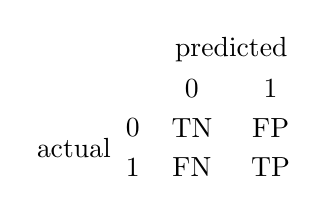
\begin{tikzpicture}
	\node at (1,3) {predicted};
	\node at (0.5,2.5) {$0$};
	\node at (1.5,2.5) {$1$};
	\node at (0.5,2) {TN};
	\node at (1.5,2) {FP};
	\node at (0.5,1.5) {FN};
	\node at (1.5,1.5) {TP};
	\node at (-0.25,2) {$0$};
	\node at (-0.25,1.5) {$1$};
	\node at (-1,1.75) {actual};
\end{tikzpicture}

\caption{confusion matrix}
\end{figure}


\cindex{receiver operating characteristic} (ROC) is a plot between \cindex{recall} and $1 - \text{specificity}$.

\cindex{PR curve} is preferred when:
\begin{itemize}
	\item positive rate is rare
	\item care more about false positive than false negative
\end{itemize}

\begin{figure}[H]
\centering	
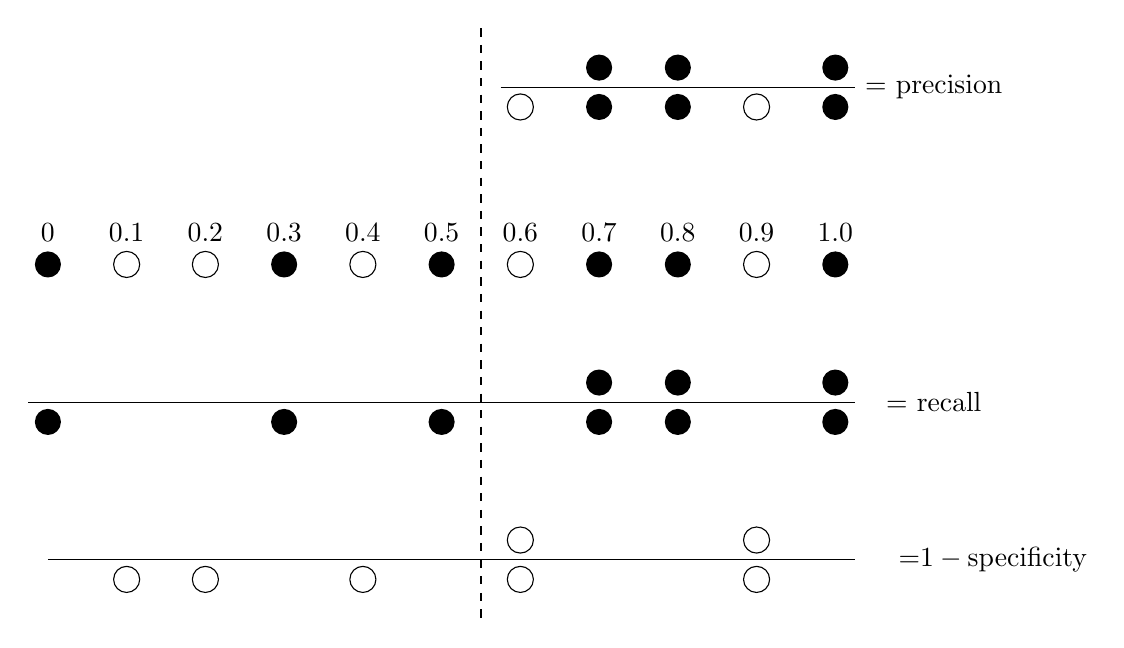
\begin{tikzpicture}
	\node [circle,fill] (s) [label=$0$] at (0,0) {};
	\node [circle,draw] (s) [label=$0.1$] at (1,0) {};
	\node [circle,draw] (s) [label=$0.2$] at (2,0) {};
	\node [circle,fill] (s) [label=$0.3$] at (3,0) {};
	\node [circle,draw] (s) [label=$0.4$] at (4,0) {};
	\node [circle,fill] (s) [label=$0.5$] at (5,0) {};
	\node [circle,draw] (s) [label=$0.6$] at (6,0) {};
	\node [circle,fill] (s) [label=$0.7$] at (7,0) {};
	\node [circle,fill] (s) [label=$0.8$] at (8,0) {};
	\node [circle,draw] (s) [label=$0.9$] at (9,0) {};
	\node [circle,fill] (s) [label=$1.0$] at (10,0) {};
	
	% draw the threshold
	\draw [dashed] (5.5,3) -- (5.5,-4.5);
	
	% draw precision
	\node [circle,draw] (s) at (6,2) {};
	\node [circle,fill] (s) at (7,2) {};
	\node [circle,fill] (s) at (8,2) {};
	\node [circle,draw] (s) at (9,2) {};
	\node [circle,fill] (s) at (10,2) {};
	
	\draw (5.75,2.25) -- (10.25,2.25);

	\node [circle,fill] (s) at (7,2.5) {};
	\node [circle,fill] (s) at (8,2.5) {};
	\node [circle,fill] (s) at (10,2.5) {};
	
	\node at (11.25,2.25) {= precision};
	
	% draw recall
	\node [circle,fill] (s) at (0,-2) {};
	\node [circle,fill] (s) at (3,-2) {};
	\node [circle,fill] (s) at (5,-2) {};
	\node [circle,fill] (s) at (7,-2) {};
	\node [circle,fill] (s) at (8,-2) {};
	\node [circle,fill] (s) at (10,-2) {};
	
	\draw (-0.25,-1.75) -- (10.25,-1.75);
	
	\node [circle,fill] (s) at (7,-1.5) {};
	\node [circle,fill] (s) at (8,-1.5) {};
	\node [circle,fill] (s) at (10,-1.5) {};
	
	\node at (11.25,-1.75) {= recall};
	
	% ROC
	
	\node [circle,draw] (s) at (1,-4) {};
	\node [circle,draw] (s) at (2,-4) {};
	\node [circle,draw] (s) at (4,-4) {};
	\node [circle,draw] (s) at (6,-4) {};
	\node [circle,draw] (s) at (9,-4) {};
	
	\draw (0,-3.75) -- (10.25,-3.75);
	
	\node [circle,draw] (s) at (6,-3.5) {};
	\node [circle,draw] (s) at (9,-3.5) {};
	
	\node at (12,-3.75) {=$1 - \text{specificity}$};
\end{tikzpicture}
\caption{PR and ROC curve}
\end{figure}

\subsection{Prediction Output Format}

\begin{description}
	\item [binary] the output is binary: $O \in \{ 0, 1\}$. such as \cindex{SVM}. 
	\item [multiclass] output can be of $n$ value: $O \in \{ 0,1,2,3\}$
		\begin{itemize}
			\item OvA: binary classifier that use one feature against all the rest feature. $n$ internal classifiers. select the one with highest score.
			\item OvO: for every feature pair, run a binary classifier. $\binom{n}{2}$ internal classifiers. select the one with highest sum of scores.
			\begin{itemize}
				\item training set needs to be small
				\item usually for \cindex{SVM}
			\end{itemize}
		\end{itemize}
	\item [multilabel] $n$ binary prediction: $[0,1,0,1]$, which means female=false, alice=true, etc. such as k-nearest neighbor. 
	\item [multioutput] $n$ non-binary output: $[1,2,89]$.
\end{description}


\subsection{Optimization}

\subsubsection{Batch Gradient Descent}

\cindex{Gradient descent} is used to minimize cost function. \cindex{Linear regression model} is \cindex{convex}, so it will be guaranteed to find global minimum.

all features need to have a similar scale in order to increase converge speed.

In GD learning, $\eta$ is the learning rate, $\theta$ is model's parameter vector, $f$ (such as MSE) is the cost function. Formula (\ref{gdlearning}) will try to minimize cost function recursively until $|\nabla_\theta f| < \varepsilon$ ($\varepsilon$ is called \cindex{tolerance})

\begin{equation}\label{gdlearning}
	\theta \gets \theta - \eta \nabla_\theta f
\end{equation}

Each iteration will use all input because the cost function is the sum of error over all inputs. So it is called \cindex{batch} and slow on very large data set.

\subsubsection{Stochastic Gradient Descent}

In each iteration just take a random instance in training set. The cost function will fluctuate. 

The SGD has the chance of finding global minimum. The \cindex{learning rate} needs to be reduced gradually in order to let the training converge, which is called \cindex{simulated annealing} process with \cindex{learning schedule}.

\subsubsection{Mini-batch Gradient Decent}

Mini-batch gradient descent the middle between SGD and GD. Each iteration will take a small random set of instance from training set.


\subsection{Learning Curve}

\cindex{Learning curve} is a plot of error against training set size for training set and validation set. 

At the beginning the error for training set is low and gradually increases, and for validation set it is high and gradually decreases. the gap between two sets could be decomposed into 3 components:
\begin{description}
	\item [bias] the model is wrong. usually \cindex{underfit}.
	\item [variance] has excessive parameter. usually \cindex{overfit}
	\item [irreducible error] data is noisy. need to clean data.
\end{description}


\subsection{Regularization}

\subsubsection{Ridge Regression}

also called \cindex{Tikhonov regularization} or $l2$ . It add the following to the cost function:
\begin{equation}
	\alpha \sum_{i=1}^n \theta_i^2
\end{equation}

The extra cost is only added during training and removed in evaluation.

The data set need to be scaled before applying \cindex{ridge regression}.

\subsubsection{Lasso Regression}
\cindex{Lasso regression} (Least absolute shrinkage and selection operator regression) will add the following to the cost function:
\begin{equation}
	\alpha \sum_{i=1}^n |\theta_i|
\end{equation}

unimportant features will have $0$ weight, so it will output a \cindex{sparse model}.

\subsubsection{Elastic Net}
\cindex{Elastic net} is the middle between \cindex{ridge regression} and \cindex{Lasso regression}. It will add the following to cost function:

\begin{equation}
	\frac{1-r}{2} \alpha \sum_{i=1}^n \theta_i^2 + r \alpha \sum_{i=1}^n |\theta_i|
\end{equation}


\subsubsection{Early Stopping}

It stops training when the validation error reaches minimum. 

For mini-batch and stochastic GD, the validation error curve will fluctuate. One solution is to continue run for a while and roll back to previous minimum.


\subsection{Logistic Regression}

\cindex{logistic regression} is a binary classifier. The probability is:

\begin{equation}
	\hat{p} = \frac{1}{1+e^{-\mathbb{\theta}^T  \mathbf{X}}}
\end{equation}

The prediction is:
\begin{equation}
	\hat{y} = \begin{cases}
		0 \text{, if } \hat{p} < 0.5 \\
		1 \text{, if } \hat{p} \geq 0.5
	\end{cases}
\end{equation}

The cost function is:
\begin{equation}
	J(\theta) = - \frac{1}{m} \sum_{i=1}^m \Big\{ y^{(i)} \log \hat{p}^{(i)} + (1-y^{(i)}) \log (1-\hat{p}^{(i)}) \Big\}
\end{equation}

The derivative is:
\begin{equation}
	\frac{\partial J(\theta)}{\partial \theta_j} = \frac{1}{m} \sum_{i=1}^m \Big( \frac{1}{1+e^{-\mathbb{\theta}^T \mathbf{X}^{(i)}}} - y^{(i)} \Big) x_j^{(i)}
\end{equation}


\subsection{Softmax Regression}
\cindex{Softmax regression} is a multiclass version of \cindex{logistic regression} which is defined as:

\begin{equation}
	\hat{p}_k = \frac{e^{\theta_k^T \mathbb{X}}}{\sum\limits_{j=1}^{\mathbf{K}} e^{\theta_j^T \mathbf{X}}}
\end{equation}

Here $\mathbb{K}$ is the number of classes.


The prediction is:
\begin{equation}
	\hat{y} = \underset{k}{\text{argmax }} \theta_k^T \mathbf{X}
\end{equation}

The cost function is:
\begin{equation}
	J(\theta)= -\frac{1}{m} \sum_{i=1}^m \sum_{k=1}^K y_k^{(i)} \log \hat{p}_k^{(i)}
\end{equation}


The gradient vector is:
\begin{equation}
	\nabla_{\theta_k} J(\theta) = \frac{1}{m} \sum_{i=1}^m(\hat{p}_k^{(i)} - y_k^{(i)}) \mathbf{X}^i
\end{equation}
\section{Classic Models}

\subsection{Linear Regression}

\subsection{Logistic Regression}

\subsection{Softmax Regression}

\subsection{SVM}

\subsection{Decision Trees}

\subsection{Ensemble Learning}

\subsubsection{Voting Classifiers}

A list of sufficiently diverse weak classifiers. It may have high success chance by the law of large numbers. There are two types:

\begin{description}
	\item [\cindex{hard voting}] majority vote
	\item [\cindex{soft voting}] select highest average probability over all classifiers
\end{description}

\subsubsection{Bagging and Pasting}

One training algorithm but with different subset of training set. There are two different ways:

\begin{description}
	\item [\cindex{bagging}] random sample with replacement. put things back
	\item [\cindex{pasting}] random sample without replacement. do not put things back
\end{description}

bagging is more diverse so it has higher bias but lower variance. Overall bagging is better than pasting.

\cindex{out-of-bag evaluation}: if there are $n$ samples, each classifier will also sample $n$ sample with replacement, which will choose $1 - e^{-1} \approx 63.2\%$ samples. The remaining could be used as test test.


\subsubsection{AdaBoost}


\subsubsection{Gradient Boosting}

In \cindex{gradient boosting} there is a series of models $\mathbf{F}_i$:

\begin{equation}
	\begin{aligned}
		\mathbf{F}_1 &\approx (\mathbf{X},\mathbf{Y}) \\
		\mathbf{F}_2 &\approx \Big(\mathbf{X},\mathbf{Y} - \mathbf{F}_1 (\mathbf{X}) \Big ) \\
		&\dots \\
		\mathbf{F}_n &\approx \Big(\mathbf{X},\mathbf{Y} - \mathbf{F}_{n-1} (\mathbf{X}) \Big )
	\end{aligned}
\end{equation}

It is called \cindex{gradient} because it is a gradient descent process. Suppose the loss function is:
\begin{equation}
	\mathcal{L}(\mathbf{Y},\mathbf{F}_k) = \frac{1}{2} \sum_i \Big ( y_i - \mathbf{F}_k (x_i) \Big )^2
\end{equation}

Suppose the aggregate function $\mathcal{F}_i = \sum\limits_i \mathbf{F}_i $, the derivative is:
\begin{equation}
	\begin{aligned}
		\frac{\partial \mathcal{L}(\mathbf{Y},\mathbf{F}_k)}{\partial \mathbf{F}(x_i)} &= \mathbf{F}_k (x_i) - y_i \\
		y_i - \mathbf{F}_k (x_i) &= - \frac{\partial \mathcal{L}(\mathbf{Y},\mathbf{F}_k )}{\partial \mathbf{F}_k (x_i)}\\
		\mathcal{F}_2 &= \mathbf{F}_1 + \mathbf{F}_2 \\
		&= \mathbf{F}_1 + y_i - \mathbf{F}_1 \\
		&= \mathbf{F}_1 - 1 \times \frac{\partial \mathcal{L}(\mathbf{Y},\mathbf{F}_1 )}{\partial \mathbf{F}_1 (x_i)} \\
		&= \mathcal{F}_1 - 1 \times \frac{\partial \mathcal{L}(\mathbf{Y},\mathcal{F}_1 )}{\partial \mathcal{F}_1 (x_i)} 
	\end{aligned}
\end{equation}

So it is a gradient descent process.


\subsubsection{Stacking}



\chapter {Deep Neural Network}


\chapter{Reinforement Learning}

\section{Background}


\subsection{State}

\cindex{environment} has state $S_t^e$, which receives action $A_t$ and emits observation $O_{t+1}$ and scalar reward $R_{t+1}$.


\cindex{state} is a function of all history, so the reinforcement learning could be a Markov process:
\begin{equation}
	S_t = f([O_1, R_1, A_1, \dots, A_{t-1}, O_t, R_t])
\end{equation}

\subsection{Planning and Learning}

\subsubsection{Planning}

\cindex{planning} uses simulated experience from \cindex{model}. So the model is known.

There are two different planning methods:
\begin{description}
	\item[\cindex{state-space planning}] searches through state space.
	\item[\cindex{plan-space planning}] searches through plans. It uses evolutionary methods. Seldom used in reinforcement learning.

\end{description}

\subsubsection{Learning}
\cindex{learning} uses real experience of environment. So the environment and policy are unknown.


\subsection{Agent}

\cindex{agent} has three important components:
\begin{itemize}
	\item policy
	\item value function
	\item model
\end{itemize}

\subsubsection{Policy}

\cindex{policy} can be deterministic or statistics :
\begin{description}
	\item[deterministic] $a = \pi(s)$ 
	\item[stochastic] $\pi(a|s) = \mathbb{P}[A_t=a|S_t=s]$
\end{description}


\subsubsection{Model}
\cindex{model} is anything an agent can use to predict environment response. so a model simulate environment.

\begin{description}
	\item[distribution model] explores all possibility and all probability
	\item[sample model] explores only one possibility
\end{description}

\cindex{distribution model} is stronger than \cindex{sample model} because it can always generate sample. However in practice it is much easier to obtain sample models.

\subsection{Evaluation and Control}

\begin{description}
	\item[\cindex{evaluation}] tries to calculate $v(s)$ or $q(s,a)$.
	\item[\cindex{control}] tries to calculate $v_*(s)$ , $q_*(s,a)$ or $\pi_*$.
\end{description}


\subsection{Exploration and Exploitation}

\begin{description}
	\item[\cindex{exploration}] find more information about environment.
	\item[\cindex{exploitation}] exploit known information to maximize reward.
\end{description}

\subsection{Incremental Mean}

If $Q_{n+1}$ is the mean of $R_i$: $Q_{n+1} = \frac{1}{n} \sum\limits_{i=1}^n R_i$. $Q_{n+1}$ could be rearrange as:
\begin{equation}
	Q_{n+1} = Q_n + \frac{1}{n} \Big( R_n - Q_n \Big)
\end{equation}

If we replace $\frac{1}{n}$ by $\alpha$, the formula becomes:
\begin{equation}
	\begin{aligned}
		Q_{n+1} &= Q_n + \alpha \Big( R_n - Q_n \Big)\\
		&= (1-\alpha )^n Q_1 + \sum_{i=1}^n \alpha (1 - \alpha )^{n-1}R_i
	\end{aligned}
\end{equation}

$Q_n$ will be convergent if $\alpha$ follows the following formula:
\begin{equation}\label{convergenceofsequence}
	\begin{cases}
		\sum\limits_{n=1}^\infty \alpha_n = \infty \\
		\\
		\sum\limits_{n=1}^\infty \alpha_n^2 < \infty
	\end{cases}
\end{equation}


\subsection{Terminology}

\cindex{backup} uses future return to update current value.




%
% section for MDP
%

\section{Markov Decision Process}

\subsection{Definition}

A \cindex{Markov decision process} (MDP) is a Markov reward process with decisions. It is an environment in which all stated are Markov. It is a tuple $\langle \mathcal{S}, \mathcal{A}, \mathcal{R}, \mathcal{P}, \gamma \rangle$:

\begin{itemize}
	\item $\mathcal{S}$ is a finite set of states.
	\item $\mathcal{A}$ is a finite set of actions.
	\item $\mathcal{R}$ is a reward function.
	\item $\mathcal{P}$ is a state transition probability matrix.
	\item $\gamma \in [0,1]$ is a discount factor.
\end{itemize}

\subsection{Goals and Equations}

\subsubsection{Environment}

\cindex{environment} has \cindex{state} $S_t \in \mathcal{S}$ and generate \cindex{reward} $R_{t+1} \in \mathbb{R}$. Anything that cannot be changed arbitrarily by the agent is part of environment. The goal of reinforcement learning is to maximize expected value of cumulative sum of received scalar reward.

The reward signal should be chosen so it will not affect how agent act.

\subsubsection{Agent}

\cindex{agent} has \cindex{action} $A_t \in \mathcal{A}(S_t)$ and \cindex{observation} $O_t$ of state $S_t$. Agent may know everything about how the environment works but still unable to solve problem, such as the Rubik cube puzzle.

\subsubsection{State and Reward}

The probability of next state and reward is :
\begin{equation}
	p(s^\prime,r|s,a) = \mathbb{P}\{S_t=s',R_t=r|S_{t-1}=s,A_{t-1}=a\}
\end{equation}

The \cindex{state-transition probabilities} is :
\begin{equation}
	p(s'|s,a)=P\{S_t=s'|S_{t-1}=s,A_{t-1} = a \}=\sum_{r \in \mathbb{R}} p(s',r|s,a)
\end{equation}





Usually the state and reward probability will be treated as independent, so their formulas are:

\begin{equation}
	\mathcal{P}_{s,s'}^a = \mathbb{P}[S_{t+1}=s' | S_t = s, A_t = a]
\end{equation}


\begin{equation}
	\mathcal{P}_{s,s'}^{\pi} = \sum_{a \in A(s)} \pi(a|s) \mathcal{P}_{s,s'}^a
\end{equation}


\begin{equation}
	\mathcal{R}_s^a = \mathbb{E}[R_{t+1}|S_t =s, A_t=a]
\end{equation}


\begin{equation}
	\mathcal{R}_s^\pi = \sum_{a \in A(s)} \pi(a|s) \mathcal{R}_s^a
\end{equation}



The expected reward of state-action pair is:
\begin{equation}
	r(s,a) = \mathbb{E}[R_t|S_{t-1}=s,A_{t-1}=a]= \sum_{r \in \mathbb{R}} \sum_{s' \in \mathbf{S}} p(s',r|s,a)
\end{equation}

\subsubsection{Episode}
An \cindex{episode} is an order sequence of $S_0, A_0,R_1,S_1,A_1, \dots, R_n, S_n$ in MDP. So an \cindex{episode} will always end.

\cindex{continuing task} is a list of actions that never terminate.

Episode task can be converted to continuing task by appending infinite \cindex{absorbing state}.


\subsubsection{Goal}
The \cindex{expected return} is the sum of rewards in the episode:
\begin{equation}
	G_t=R_{t+1}+R_{t+2} + R_{t+3} +\dots + R_T
\end{equation}

\begin{itemize}
	\item \cindex{terminal state}: $R_T$ 
	\item $S$: All non-terminal states
	\item $S^+$: all terminal and non-terminal states
\end{itemize}


\cindex{discounted return} for continuing task is defined as:
\begin{equation}
	\begin{aligned}
		G_t&=R_{t+1}+\gamma R_{t+2} + \gamma^2 R_{t+3} + \dots  \\
		&= \sum_{k=0}^\infty \gamma^k R_{t+k_1} \\
		&= R_{t+1} + \gamma G_{t+1}
	\end{aligned}
\end{equation}

where $0 \leq \gamma \leq 1$.


\subsubsection{Policy}

A stochastic policy is a probability of selecting next possible action:

\begin{equation}
	\pi(a|s)=\mathbb{P}[A_t = a | S_t = s]
\end{equation}

\subsubsection{Value Function}

The \cindex{state-value} function $V_\pi$ for policy $\pi$ is:

\begin{equation}
	\begin{aligned}
		V_{\pi}(s) &= \mathbb{E}_{\pi}[G_t|S_t=s] \\
		&=\mathbb{E}[R_{t+1} + \gamma V_{\pi}(S_{t+1})| S_t = s]
	\end{aligned}
\end{equation}

The \cindex{action-value} function $q_\pi$ for policy $\pi$ is:

\begin{equation}
	\begin{aligned}
		q_{\pi}(s,a) &= \mathbb{E}_{\pi}[G_t|S_t=s,A_t=a] \\
					&= \mathbb{E}[R_{t+1} + \gamma q_{\pi}(S_{t+1}, A_{t+1})| S_t = s, A_t = a]
	\end{aligned}
\end{equation}

\subsubsection{Bellman Equation}


Bellman equation (\cindex{backup} process) is an expansion of value function:

\begin{equation}\label{bellman:v}
	\begin{aligned}
		V_{\pi}(s) &= \sum_{a \in \mathcal{A}(s)} \pi(a|s) q_{\pi}(s,a) \\
		&= \sum_{a \in \mathcal{A}(s)} \pi(a|s) \left( \mathcal{R}_s^a + \gamma \sum_{s' \in \mathcal{S}} \mathcal{P}_{s,s'}^a V(S') \right)
	\end{aligned}
\end{equation}

\begin{equation}
	\begin{aligned}
		q_{\pi}(s,a) &= R_s^a + \gamma \sum_{s' \in \mathcal{S}} \mathcal{P}_{s,s'}^a V_{\pi}(s') \\
		&= R_s^a + \gamma \sum_{s' \in \mathcal{S}} \mathcal{P}_{s,s'}^a \left( \sum_{a', s'} \pi(a'|s') q_{\pi}(s',a') \right )
	\end{aligned}
\end{equation}



\subsubsection{Bellman Equation Solution}

Formula (\ref{bellman:v}) is for a single state. Let 
\begin{equation}
	V_{\pi} = \left [\begin{matrix}
 	V_{\pi}(s_1) \\
 	\vdots \\
 	V_{\pi}(s_n)
 \end{matrix} \right ]
\end{equation}

Formula (\ref{bellman:v}) now becomes:

\begin{equation}
	\mathbf{V}_{\pi}=\mathbf{R}^{\pi} + \gamma \mathbf{P}^{\pi} \mathbf{V}_{\pi} 
\end{equation}

So the solution to \cindex{Bellman Equation} is:

\begin{equation}
	\mathbf{V}_{\pi}=(\mathbf{I} - \gamma \mathbf{P}^{\pi})^{-1}\mathbf{R}^{\pi}
\end{equation}

It is a fixed point solution to formula (\ref{bellman:v}).

\subsection{Optimal Policy}

\subsubsection{Policy Partial Order}

$\pi \geq \pi^{\prime}$ if $\forall s \in \mathcal{S}, V_{\pi} (s) \geq V_{\pi^{\prime}} (s)$ . 


For MDP all optimal solution share the same value function $V_*$ and include at least one deterministic policy $\pi_*$. 


\subsubsection{Optimal State-value Function}

The optimal state-value function $V_*$ is defined as:


\begin{equation}
	\begin{aligned}
		V_*(s) &= \underset{\pi}{\max} \ V_{\pi}(s) \\
		&= \underset{a}{\max}\ q_* (s, a) \\
		&= \underset{a}{\max}\ \left( \mathcal{R}_s^a + \gamma \sum_{s' \in \mathcal{S}} \mathcal{P}_{s,s'}^a V_*(s') \right )
	\end{aligned}
\end{equation}

\subsubsection{Optimal Action-value Function}


The optimal action-value function $q_*$ is defined as:

\begin{equation}
	\begin{aligned}
		q_*(s,a)&=\underset{\pi}{\max}\ q_{\pi}(s,a)\\
		&=\mathbb{E}[R_{t+1}+\gamma V_*(S_{t+1})|S_t=s, A_t=a]\\		
		&=\mathcal{R}_s^a+\gamma \sum_{s' \in \mathcal{S}} \mathcal{P}_{s,s'}^a V_*(s')\\
		&=\mathcal{R}_s^a+\gamma \sum_{s' \in \mathcal{S}} \mathcal{P}_{s,s'}^a \ \underset{a'}{\max}\  q_*(s',a')
	\end{aligned}
\end{equation}

Here $\mathcal{R}_s^a$ is an expectation. In model-free learning and controlling it is the sample return from environment.

\subsubsection{Optimal Policy from Action Value Function} Once the optimal action value function is known, we can calculate the optimal policy by:

\begin{equation}\label{optimal:policy}
	\pi_*(a|s) =
	\begin{cases}
		1& \text{, if $a = \underset{a \in \mathcal{A}(s)}{\text{argmax}}\ q_*(s,a)$}\\
		0& \text{, else}
	\end{cases}
\end{equation}

So the optimal policy is a greedy algorithm.

Compared with $V_*$, $q_*$ is better because it does not need to do one step lookahead.

\subsubsection{Reason for Complex Algorithms}

There is no closed form for optimal Bellman policy equation, so many iterative solution exists:
\begin{itemize}
	\item value iteration
	\item policy iteration
	\item $Q$-learning
	\item Sarsa
\end{itemize}





\section{Dynamic Programming}

DP are effective for medium size problems (million of states).

\subsection{Policy Evaluation (Prediction)}

If $P$ and $\pi$ are known, Bellman equation (\ref{bellman:v}) could be converted to iterative solution. All $V$ are randomly initialized and updated using \cindex{iterative policy evaluation}:

\begin{equation}
	V_{k+1} (s) = \sum_a \pi (a | s) \left ( \sum_{s',r} p(s',r | s,a) \Big ( r + \gamma V_{k}(s') \Big ) \right )
\end{equation}

Here $V_{t+1}(s)$ means the value of $V(s)$ in $(t+1)$ round.

There are two ways to update $V_{t+1}(s)$:
\begin{itemize}
	\item copy $V_{t+1}(s)$ to a new array and update original array when sweeping is done
	\item \cindex{in-place} update: update $V(s)$ on the fly. updated value may be used immediately so it is faster than two array solution.
\end{itemize}


The problem is that iterative algorithm \cindex{sweep} through all state space, which might not be practical.

See Algorithm (\ref{algo:itepole}) for detail.

\begin{algorithm}
	\caption{Iterative policy evaluation, estimate $V_\pi$}\label{algo:itepole}
	
	\begin{algorithmic}[1]
		\Procedure{}{$\pi, p, \theta$}
			\State $\forall s \in S, V(s) \gets random$
			\State $V(terminal) \gets 0$
			\Repeat
				\State $\Delta \gets 0$
				\For{$s \in S$}
					\State $v \gets V(s)$
					\State \Comment{in-place update}
					\State $V(s) \gets \sum\limits_a \pi (a | s) \left ( \sum\limits_{s',r} p(s',r | s,a) \big(r + \gamma V(s') \big ) \right )$ 
					\State $\Delta \gets \max{}(v, |v - V(s)|)$
				\EndFor
			\Until{$\Delta < \theta$}
		\EndProcedure
	\end{algorithmic}

\end{algorithm}


\subsection{Policy Improvement}

The reason for calculating value function is to help find a better policy. A new greedy policy $\pi^{\prime}$ could be calculated using:

\begin{equation}
	\begin{aligned}
		\pi^{\prime}(s) &= \underset{a \in \mathcal{A}(s)}{\text{argmax}} \ q_{\pi}(s,a)\\
		&=\underset{a \in \mathcal{A}(s)}{\text{argmax}}\ \sum_{s',r} p(s',r|s,a)\Big ( r+\gamma V(s') \Big )
	\end{aligned}
\end{equation}

A series of policy evaluation and improvement will converge to optimal result, and its conversion is very fast. 

The drawback is that every iteration may trigger evaluation, which involves multiple sweep through all state space.

See Algorithm (\ref{algo:polite}) for detail.


\begin{algorithm}
	\caption{Policy Iteration, estimate $V_*$ and $\pi_*$}\label{algo:polite}
	
	\begin{algorithmic}[1]
		\State $\forall s \in \mathcal{S}, V(s) \gets random$
		\State $V(terminal) \gets 0$
		\State $\pi(s) \gets \text{random}(\mathcal{A}(s))$
		
		\Statex
		
		\Procedure{PolicyEvaluation}{$\varepsilon$}
			\Repeat
				\State $\Delta \gets 0$
				\For{$s \in \mathcal{S}$}
					\State $v \gets V(s)$
					\State $V(s) \gets \sum\limits_{s',r} p(s',r|s,\pi(s))\big (r+\gamma V(s') \big )$ \Comment{$\pi(s)$ : use optimal policy}
					\State $\Delta \gets \max (\Delta, |v - V(s)|)$
				\EndFor
			\Until{$\Delta < \varepsilon$}
		\EndProcedure
		
		\Statex
		
		\Procedure{PolicyImprovement}{}
			\State $\text{stable} \gets \text{TRUE}$
			\For{$s \in \mathcal{S}$}
				\State $old \gets \pi(s)$
				\State $\pi(s) \gets \underset{a \in \mathcal{A}(s)}{\text{argmax}}\ \sum\limits_{s',r}P(s',r|s,a) \big (r+\gamma V(s') \big )$
				\If{$old \neq \pi(s)$}
					\State $\text{stable} \gets \text{FALSE}$
				\EndIf
			\EndFor
			\If{$\text{stable}$}
				\Return $(V_*,\pi_*)$
			\Else
				\State \Call{PolicyEvaluation}{$\varepsilon$} \Comment{update $V$ if optimal policy has changed}
			\EndIf
		\EndProcedure
	\end{algorithmic}
\end{algorithm}

\subsection{Value Iteration}

In policy iteration, multiple sweep can be reduce to one by taking the best action, and calculate optimal policy using (\ref{optimal:policy}):

\begin{equation}
	\begin{aligned}
		V_{k+1}^{old} (s) &= \sum_{s',r} p(s',r|s,\pi(s))\big (r+\gamma V_k(s') \big ) \\
		V_{k+1}^{new} (s) &= \underset{a}{\max} \sum_{s',r} p(s',r|s,a) \big (r+\gamma V_k(s') \big )
	\end{aligned}
\end{equation}

See Algorithm (\ref{algo:valite}) for detail.

\begin{algorithm}
	\caption{Value Iteration, estimate $\pi_*$}\label{algo:valite}
	
	\begin{algorithmic}[1]
		\State $\forall s \in S, V(s) \gets random$
		\State $V(terminal) \gets 0$
		
		\Statex
		
		\Repeat
			\State $\Delta \gets 0$
			\For{$s \in S$}
				\State $v \gets V(s)$
				\State \Comment policy evaluation and improvement
				\State $V(s) \gets \underset{a}{\max}\ \sum\limits_{s',r} p(s',r|s,a) \big ( r+\gamma V(s') \big )$ 
				\State $\Delta \gets \max (\Delta, |v - V(s)|)$
			\EndFor
		\Until{$\Delta < \theta$}
		
		\State \Return $\pi_*(s)= \underset{a}{\text{argmax}} \ \sum\limits_{s',r} p(s',r|s,a) \big (r+\gamma V(s') \big )$
	\end{algorithmic}
\end{algorithm}

\subsection{Generalized Policy Iteration}

\cindex{Generalized Policy Iteration} (GPI) is a series of evaluation and improvement process. Almost all reinforcement learning methods are GPI.


\subsection{Performance}

DP is exponentially faster than direct \cindex{policy space search}.

DP is better than \cindex{linear programming methods} for large problem, but worse for small problem.


The \cindex{curse of dimension} is not the problem of algorithm but the problem itself.

The time complexity for $v$ is $O(mn^2)$ and for $q$ is $O(m^2 n^2)$, where $m$ is the number of action and $n$ is the number of state. So DP is effective for medium size problems (million of states).

\subsection{Extension to Sweeping}

\subsubsection{Prioritized Sweeping}

backup the state with the maximum \cindex{Bellman error}:
\begin{equation}
	\left| \max_{ a \in \mathcal{A}} \left( \mathcal{R}
	+ \gamma \sum_{s' \in S} \mathcal{P}_{ss'}^a v(s') \right) - v(s) \right|
\end{equation}

\subsubsection{Realtime Dynamic Programming}

Choose the state that are relevant to agent.




\section{Monte Carlo Methods}

\subsection{Requirement}

\begin{itemize}
	\item need episode, so need to terminate
	\item start only when episode ends
	\item do not need model
\end{itemize}

Note: Monte Carlo Method is not a online method because it is not step-by-step method.

\subsection{Prediction}

\subsubsection{First Visit MC}

\cindex{Monte Carlo} prediction has \cindex{first visit} and \cindex{every visit} methods.


The \cindex{first visit} Algorithm (\ref{algo:fvmc}) is an unbiased estimate. 



\begin{algorithm}
	\caption{First visit MC, estimate $v_\pi$}\label{algo:fvmc}
	
	\begin{algorithmic}[1]
		\State $\forall s \in \mathcal{S}, V(s) \gets random$
		\State $\text{Returns}(s) \gets []$
		
		\Statex
		
		\Loop
			\State generate an episode $\pi: S_0, A_0, R_1, S_1, A_1, R_2, \dots, S_{T-1}, A_{T-1}, R_T$
			\State $G \gets 0$
			\For{$t \gets T-1, T-2, \dots, 0$}
				\State $G \gets \gamma G + R_{t+1}$
				
				\Comment{loop backward to find first appearance}
				\If{$S_t \notin \{S_0, S_1, \dots, S_{t-1}\}$}
					\State $\text{Returns}(S_t) \gets \text{Returns}(S_t) + G$
					\State $V(S_t) \gets \text{average}(\text{Returns}(S_t))$
				\EndIf
			\EndFor
		\EndLoop
	\end{algorithmic}
\end{algorithm}

\subsection{Explore All State-Action Pair}

In Monte Carlo control, the policy at $S_t$ need to explore all $q(S_t,A_t)$, which means the MC algorithm needs to cover all $\langle S_t, A_t \rangle$ pairs. There are two ways to achieve this:

\begin{itemize}
	\item exploring start. It might not be possible to enumerate all start.
	\item $\varepsilon$-soft policy.
\end{itemize}

\subsubsection{Exploring Starts}

It tries all $\langle S_t, A_t \rangle$ pairs as the first action. See Algorithm (\ref{algo:estart}) for detail.

If model is not available, $q_\pi$ is preferred than $V_\pi$ because it does not need transition probability when calculating optimal policy. 


\begin{algorithm}
	\caption{first visit MCES (Exploring Starts), estimate $\pi_*$}\label{algo:estart}	
	
	\begin{algorithmic}[1]
		\State $\pi(s) \in \mathcal{A}(s)$
		\State $q(s,a) \in \mathbb{R}$
		\State $\text{Returns}(s,a) \gets []$
		
		\Statex
		
		\Loop
			\State choose $S_0$ and $A_0$ so all pairs will appear \Comment{exploring starts}
			\State generate episode from $\langle S_0,A_0 \rangle$: $\pi: S_0, A_0, R_1,\dots, S_{T-1}, A_{T-1}, R_T$
			\State $G \gets 0$
			
			\For{$t \gets T-1, T-2, \dots, 0$}
				\State $G \gets \gamma G + R_{t+1}$
				
				\If{$\langle S_t, A_t \rangle \notin \{\langle S_0,A_0 \rangle,\langle S_1,A_1 \rangle, \dots,\langle S_{t-1}, A_{t-1} \rangle \}$}
					\State $\text{Returns}(S_t, A_t) \gets \text{Returns}(S_t, A_t) + G$
					\State $q(S_t, A_t) \gets \text{average}(\text{Returns}(S_t, A_t))$
					\State $\pi (S_t) \gets \underset{a \in \mathcal{A}(S_t)}{\text{argmax}}\ q(S_t, a) $
				\EndIf
			\EndFor
		\EndLoop
	\end{algorithmic}
\end{algorithm}

\subsubsection{$\varepsilon$-soft Policy}

In $\varepsilon$-soft policy, all $\langle S_t, A_t \rangle$ pairs are tried in the middle with non-zero probability:

\begin{itemize}
	\item \cindex{$\varepsilon$-soft} : $\pi(a|s) > \frac{\varepsilon}{\mathcal{A}(s)}$.
	\item \cindex{$\varepsilon$-greedy} : see Algorithm (\ref{algo:fvmcsoft}) for detail.
\begin{equation*}
	\pi(a|s) = 	
		\begin{cases}
				\frac{\varepsilon}{\mathcal{A}(s)} & \text{, if } a \text{ is not the greedy choice} \\
				1 - \varepsilon + \frac{\varepsilon}{\mathcal{A}(s)} & \text{, if } a  \text{ is the greedy choice}
		\end{cases}
\end{equation*}
\end{itemize}



\begin{algorithm}
	\caption{first visit MC control ($\varepsilon$-greedy), estimate $\pi_*$}\label{algo:fvmcsoft}	
	
	\begin{algorithmic}[1]
		\State $\pi \gets $ random $\varepsilon$-greedy policy
		\State $q(s,a) \in \mathbb{R}$
		\State $\text{Returns}(s,a) \gets []$
		
		\Statex
		
		\Loop
			\State choose $S_0$ and $A_0$ \Comment{non-exploring start}
			\State generate episode from $\langle S_0,A_0 \rangle$: $\pi: S_0, A_0, R_1, \dots, S_{T-1}, A_{T-1}, R_T$
			\State $G \gets 0$
			
			\For{$t \gets T-1, T-2, \dots, 0$}
				\State $G \gets \gamma G + R_{t+1}$
				
				\If{$\langle S_t, A_t \rangle \notin \{\langle S_0,A_0 \rangle,\langle S_1,A_1 \rangle, \dots,\langle S_{t-1}, A_{t-1} \rangle \}$}
					\State $\text{Returns}(S_t, A_t) \gets \text{Returns}(S_t, A_t) + G$
					\State $q(S_t, A_t) \gets \text{average}(\text{Returns}(S_t, A_t))$
					\State $A^* \gets \underset{a \in \mathcal{A}(S_t)}{\text{argmax }} q(S_t, a) $
					
					\For{$a \in \mathcal{A}(S_t)$}   \Comment{$\varepsilon$-greedy}
						\State \begin{equation*}
							\pi(a|S_t) \gets \begin{cases}
								1 - \varepsilon + \frac{\varepsilon}{\mathcal{A}(s)} & \text{,if } a = A^* \\
								\frac{\varepsilon}{\mathcal{A}(s)} & \text{,if } a \neq A^*
							\end{cases} 
						\end{equation*}
					\EndFor
				\EndIf
			\EndFor
		\EndLoop
	\end{algorithmic}
\end{algorithm}

\subsection{Off-policy prediction via Importance Sampling}

\subsubsection{Target Policy}

\begin{description}
	\item[behavior policy] the policy $b$ used to generate behavior
	\item[target policy] the policy $\pi$ being learned
\end{description}

It has the assumption of \cindex{coverage}: 
\begin{equation}
	\pi(a|s) > 0 \Rightarrow b(a|s) >0
\end{equation}


\subsubsection{Importance Sampling}

The probability of $\{ A_t, S_{t+1},A_{t+1},\dots,S_T  \}$ under policy $\pi$ is (using Monte Carlo property):
\begin{equation}
	\mathbb{P} \{ A_t, S_{t+1},A_{t+1},\dots,S_T | S_t, A_{t:T-1} \sim \pi \} = \prod_{k=t}^{T-1} \pi(A_k|S_k)p(S_{k+1}|S_k,A_k)
\end{equation}

The \cindex{importance-sampling ratio} is:
\begin{equation}\label{importancsamplingratio}
	\rho_{t:T-1}^{\pi / b} = \frac{\prod\limits_{k=t}^{T-1} \pi(A_k|S_k)p(S_{k+1}|S_k,A_k)}{\prod\limits_{k=t}^{T-1} b(A_k|S_k)p(S_{k+1}|S_k,A_k)} = \prod_{k=t}^{T-1} \frac{\pi(A_k|S_k)}{b(A_k|S_k)}
\end{equation}

Let $\mathcal{T}$ denotes the set of all timestamps that $s$ is visited, $T(t)$ is the timestamp that the episode terminate following timestamp $t$, $G_t$ is the return between timestamp $t$ and $T(t)$. There are two different importance sampling:
\begin{description}
	\item [ordinary importance sampling] \begin{equation}
		V(s) = \frac{\sum\limits_{t \in \mathcal{T}} \rho_{t:T-1}^{\pi/b} G_t}{|\mathcal{T}|}
	\end{equation}
	\item [weighted importance sampling] \begin{equation}
		V(s) = \frac{\sum\limits_{t \in \mathcal{T}} \rho_{t:T-1}^{\pi/b} G_t}{\sum\limits_{t \in \mathcal{T}} \rho_{t:T-1}^{\pi/b}}
	\end{equation}
\end{description}

For \cindex{first visit} method, \cindex{Ordinary importance sampling} is unbiased, with unlimited variance. So \cindex{weighted importance sampling} is preferred in practice.

For \cindex{every visit} method, both sampling is biased which reduces to near zero when the number of sampling increases.


In practice, \cindex{every visit} is preferred because it does not need to keep trace of which states have been visited.

\subsection{Incremental Policy Evaluation}

Incremental implementation need the following background. If we want to estimate 
\begin{equation}
	V_n = \frac{\sum\limits_{k=1}^{n-1} W_k G_k}{\sum\limits_{k=1}^{n-1} W_k}, n \geq 2
\end{equation}

$V_n$ could be incrementally updated by:
\begin{equation}
	V_{n+1} = V_n + \frac{W_n}{C_n} \Big( G_n - V_n \Big), n \geq 1
\end{equation}

where 
\begin{equation*}
	C_{n+1} = C_n + W_{n+1}
\end{equation*}

Algorithm (\ref{algo:opmcp}) implements incremental solution of weighted importance sampling:

\begin{algorithm}
	\caption{off-policy MC policy evaluation, estimate $q_\pi$}\label{algo:opmcp}	
	
	\begin{algorithmic}[1]
		\State $Q(s,a) \in \mathbb{R}$
		\State $C(s,a) \in 0$
		
		\Statex
		
		\Loop
			\State $b \gets $ any policy with coverage of $\pi$
			\State generate episode following $b$: $S_0, A_0,R_1, \dots, S_{T-1},A_{T-1},R_T$
			\State $G \gets 0$
			\State $W \gets 1$
			\For{$t \gets T-1, T-2, \dots, 0$}
				\State $G \gets \gamma G + R_{t+1}$
				\State $C(S_t,A_t) \gets C(S_t,A_t) + W$ 
				\State $Q(S_t,A_t) \gets Q(S_t,A_t) + \frac{W}{C(S_t,A_t)} \Big ( G - Q(S_t,A_t) \Big)$
				\State $W \gets W \frac{\pi(A_t|S_t)}{b(A_t|S_t)}$
				
				\If{$W = 0$} \Comment{$\pi(A_t|S_t) = 0$}, $b$ does not cover $\pi$
					\State exit  For loop
				\EndIf
			\EndFor
		\EndLoop
	\end{algorithmic}
\end{algorithm}


\subsection{Incremental Policy Control}

The behavior policy $b$ need to be $\varepsilon$-soft.

Algorithm (\ref{algo:opmcpc}) implements incremental control of weighted importance sampling:

\begin{algorithm}
	\caption{off-policy MC policy control, estimate $q_*$}\label{algo:opmcpc}	
	
	\begin{algorithmic}[1]
		\State $Q(s,a) \in \mathbb{R}$
		\State $C(s,a) \in 0$
		\State $\pi(s) \gets \underset{a}{\text{argmax}} Q(s,a)$
		
		\Statex
		
		\Loop
			\State $b \gets $ any $\varepsilon$-soft policy
			\State generate episode following $b$: $S_0, A_0,R_1, \dots, S_{T-1},A_{T-1},R_T$
			\State $G \gets 0$
			\State $W \gets 1$
			\For{$t \gets T-1, T-2, \dots, 0$}
				\State $G \gets \gamma G + R_{t+1}$
				\State $C(S_t,A_t) \gets C(S_t,A_t) + W$ 
				\State $Q(S_t,A_t) \gets Q(S_t,A_t) + \frac{W}{C(S_t,A_t)} \Big( G - Q(S_t,A_t) \Big)$
				\State $\pi(S_t) \gets \underset{a}{\text{argmax}}\  Q(S_t,a)$
				
				\If{$A_t \neq \pi(S_t)$}
					\State exit  For loop
				\EndIf
				
				\State $W \gets W \frac{1}{b(A_t|S_t)}$ \Comment{$\pi(A_t|S_t) = 1$ because it is greedy}
			\EndFor
		\EndLoop
	\end{algorithmic}
\end{algorithm}


 


\section{Temporal Difference Learning}

\subsection{Constant-$\alpha$ \cindex{TD(0)} Prediction}

Suppose at time $t+1$, state becomes $S_{t+1}$ with reward $R_{t+1}$. The  \cindex{TD error} is defined as:
\begin{equation}
	\delta_t = R_{t+1} + \gamma V(S_{t+1}) - V(S_t)
\end{equation}

The simplest TD is:
\begin{equation}
	V(S_t) \gets V(S_t) + \alpha \delta_t
\end{equation}

Because TD use Markov property while MC is not, it is usually more efficient.

It use $R_{t+1} + \gamma V(S_{t+1})$ to estimate $G_t$ in formula $V(S_t) \gets V(S_t) + \alpha \Big ( G_t - V(S_t) \Big )$ which is an average of all $G_t$.

TD is \cindex{sample update} which explores just one condition while MC is \cindex{expected update} which explores all choices.

The advantage of TD:
\begin{description}
	\item [over DP] TD does not require a model of environment.
	\item [over MC] TD is an online, fully incremental fashion, more efficient.
\end{description}  

TD is sensitive to initial value (guess).


Algorithm (\ref{algo:tdpe}) contains detail.

\begin{algorithm}
	\caption{TD(0) policy evaluation, estimate $v_\pi$}\label{algo:tdpe}	
	
	\begin{algorithmic}[1]
		\State $ \alpha \in (0,1]$
		\State $V(s) \gets$ random \Comment{bootstrap}
		
		\Statex
		
		\Loop
			\State choose $S$
			\Repeat
				\State $A \gets$ action given by $\pi$ for $S$ \Comment following the given policy $\pi$
				\State take action $A$, get $R$ and $S'$
				\State $V(S) \gets V(S) + \alpha \Big (R + \gamma V(S') - V(S) \Big )$
				\State $S \gets S'$
			\Until{$S$ is terminal}
		\EndLoop		
	\end{algorithmic}
\end{algorithm}

\subsection{Sarsa: On-policy TD Algorithm}

\subsubsection{Sarsa Prediction}

\cindex{Sarsa} is a process of $S_t,A_t,R_{t+1},S_{t+1},A_{t+1}$, and its formula is:
\begin{equation}
	Q(S_t,A_t) \gets Q(S_t,A_t) + \alpha \Big ( R_{t+1} + \gamma Q(S_{t+1},A_{t+1}) - Q(S_t,A_t) \Big )
\end{equation}

If $S_{t+1}$ is terminal, then $Q(S_{t+1},A_{t+1})$ is $0$.

\subsubsection{Sarsa Control}

The algorithm is almost the same as Sarsa prediction. The difference is to update the policy on the fly using $\varepsilon$-soft or $\varepsilon$-greedy policy.

Algorithm (\ref{algo:sarsa}) contains detail.

\begin{algorithm}
	\caption{on-policy Sarsa TD control, estimate $q_*$}\label{algo:sarsa}	
	
	\begin{algorithmic}[1]
		\State $ \alpha \in (0,1]$
		\State $Q(s,a) \gets$ random
		
		\Statex
		
		\Loop
			\State choose $S$
			\State $A \gets$ action from a policy derived from $Q$ (e.g., $\varepsilon$-greedy) \Comment {update policy}
			\Repeat
				\State take action $A$, get $R$ and $S'$
				\State \Comment {update policy after each iteration}
				\State $A' \gets$ action from a policy derived from $Q$ (e.g., $\varepsilon$-greedy) 
				\State $Q(S,A) \gets Q(S,A) + \alpha \Big (R + \gamma Q(S',A') - Q(S,A) \Big )$
				\State $S \gets S'$
				\State $A \gets A'$
			\Until{$S$ is terminal}
		\EndLoop		
	\end{algorithmic}
\end{algorithm}



\subsection{Expected Sarsa Learning Algorithm}

\cindex{expected Sarsa} use expectation, rather than $\varepsilon$-greedy, to learn next $q$. It reduces variance by removing the random selection of $A_{t+1}$ during $\varepsilon$-soft policy :

\begin{equation}
	Q(S_t,A_t) \gets Q(S_t,A_t) + \alpha \left ( R_{t+1} + \gamma \sum_a \pi(a|S_{t+1}) Q(S_{t+1},a) - Q(S_t,A_t) \right )
\end{equation}


\subsection{\cindex{Q-learning}: Off-policy TD Control}

\cindex{Q-learning} is defined as:
\begin{equation}
	Q(S_t,A_t) \gets Q(S_t,A_t) + \alpha \Big ( R_{t+1} + \gamma \max_a Q(S_{t+1},a) - Q(S_t,A_t) \Big )
\end{equation}



Algorithm (\ref{algo:qlearning}) contains detail.

\begin{algorithm}
	\caption{off-policy Q-learning TD control, estimate $\pi_*$}\label{algo:qlearning}	
	
	\begin{algorithmic}[1]
		\State $ \alpha \in (0,1]$
		\State $Q(s,a) \gets$ random
		
		\Statex
		
		\Loop
			\State choose $S$
			\Repeat
				\State $A \gets$ action given by $Q$ for $S$ (e.g., $\varepsilon$-greedy)
				\State take action $A$, get $R$ and $S'$
				\State $Q(S,A) \gets Q(S,A) + \alpha \Big ( R + \gamma \underset{a}{\max}\ Q(S',a) - Q(S,A) \Big )$
				\State $S \gets S'$
			\Until{$S$ is terminal}
		\EndLoop		
	\end{algorithmic}
\end{algorithm}

\subsection{Double Learning}

Maximization has \cindex{maximization bias}. For example, if $\mathbb{E}[q(s,a)] = 0$, then $\max q(s,a) > 0$. So the selection of $q$ is always a positive bias. One way of viewing the problem is that maximization use the same sample to determine action and estimate its value. \cindex{double learning} uses two $q$ for determination and estimation.


Algorithm (\ref{algo:doublelearning}) contains detail of double q-learning TD control.

\begin{algorithm}
	\caption{double Q-learning TD control, estimate $q_*$}\label{algo:doublelearning}	
	
	\begin{algorithmic}[1]
		\State $ \alpha \in (0,1]$
		\State $Q_1(s,a) \gets$ random
		\State $Q_2(s,a) \gets$ random		
		
		\Statex
		
		\Loop
			\State choose $S$
			\Repeat
				\State $A \gets$ action given by $\varepsilon$-greedy policy of $Q_1+Q_2$ for $S$
				\State take action $A$, get $R$ and $S'$
				\State $p \gets \text{random}(0,1)$
				\If{$p > 0.5$}
					\State $Q_1(S,A) \gets Q_1(S,A) + \alpha \Big(R + \gamma Q_2(S',  \underset{a}{\max}\  Q_1(S',a)) - Q_1(S,A)\Big)$
				\Else
					\State $Q_2(S,A) \gets Q_2(S,A) + \alpha \Big(R + \gamma Q_1(S',\underset{a}{\max}\  Q_2(S',a)) - Q_2(S,A)\Big)$
				\EndIf
				\State $S \gets S'$
			\Until{$S$ is terminal}
		\EndLoop		
	\end{algorithmic}
\end{algorithm}

There are double learning version for Sarsa and Expected-Sarsa as well.


\subsection{Comments}

Compared with MC, TD is sensitive to initial value. It explores Monte Carlo property and is more effective. 


\begin{itemize}
    \item TD: average $V$ using $R + \gamma V$.
    \item Sarsa: from $V$ to $Q$.
    \item Expect Sarsa: remove randomness of Sarsa by average.
    \item Q: replace average by $\max$.
    \item Double-Q: reduce $\max$ bias by using two queues.
\end{itemize}

\section{$n$-step Bootstrapping}

\subsection{$n$-step TD Prediction}

$n$-step TD prediction is still TD because it changes earlier estimate.

It did not update anything for the first $n-1$ steps. If $t + n \geq T$, the missing terms are treated as $0$. It is defined as:

\begin{equation}
	G_{t:t+n} = R_{t+1} + \gamma R_{t+2} + \dots + \gamma^{n-1} R_{t+n} + \gamma^n V_{t+n-1}(S_{t+n})
\end{equation}


The algorithm (\ref{algo:nsteptdpredition}) contains detail.


\begin{algorithm}
	\caption{$n$-step TD prediction, estimate $v_\pi$}\label{algo:nsteptdpredition}	
	
	\begin{algorithmic}[1]
		\State $ \alpha \in (0,1]$
		\State $V(s) \gets$ random
		\State $t \gets 0$
		
		\Statex
		
		\Loop
			\State choose $S_0$
			\State $T \gets \infty$
			\While{$\tau < T - 1$}
				\If{$t < T$}
					\State take action according to $\pi(\cdot|S_t)$
					\State store $R_{t+1}$ and $S_{t+1}$
					\If{$S_{t+1}$ is terminal}
						\State $T \gets t+1$
					\EndIf
				\EndIf
				
				\State $\tau \gets t - n + 1$ \Comment $\tau$ is the pivot of update
				
				\If{$\tau \geq 0$}
					\State $G \gets \sum\limits_{i=\tau+1}^{\min (\tau+n,T)} \gamma^{i-\tau-1} R_i$ \Comment $G_{\tau:\tau+n}$
					\If{$\tau + n < T$}
						\State $G \gets G + \gamma^n V(S_{\tau + n})$
					\EndIf
					
					\State $V(S_\tau) \gets V(S_\tau) + \alpha \Big(G - V(S_\tau)\Big)$
				\EndIf

				\State $t \gets t+1$
			\EndWhile
		\EndLoop
	\end{algorithmic}
\end{algorithm}



\subsection{$n$-step Sarsa}

It is the same as $n$-step TD prediction with $q$ and $\varepsilon$-greedy. 

\begin{equation}
	G_{t:t+n} = R_{t+1} + \gamma R_{t+2} + \dots + \gamma^{n-1} R_{t+n} + \gamma^n Q_{t+n-1}(S_{t+n},A_{t+n})
\end{equation}


The algorithm (\ref{algo:nstepsarsa}) contains detail.


\begin{algorithm}
	\caption{$n$-step Sarsa, estimate $q_\pi$ or $q_*$}\label{algo:nstepsarsa}	
	
	\begin{algorithmic}[1]
		\State $ \alpha \in (0,1]$
		\State $Q(s,a) \gets$ random
		\State $\pi \gets$ random $\varepsilon$-greedy policy or a given fixed policy
		\State $t \gets 0$
		
		\Statex
		
		\Loop
			\State choose $S_0$
			\State choose action $A_0 \sim \pi (\cdot | S_0)$
			\State $T \gets \infty$
			\While{$\tau < T - 1$}
				\If{$t < T$}
					\State take action $A_t$ and store $R_{t+1}$ and $S_{t+1}$
					\If{$S_{t+1}$ is terminal}
						\State $T \gets t+1$
					\Else
						\State choose $A_{t+1} \sim \pi(\cdot|S_{t+1})$
					\EndIf
				\EndIf
				
				\State $\tau \gets t - n + 1$ \Comment $\tau$ is the pivot of update
				
				\If{$\tau \geq 0$}
					\State $G \gets \sum\limits_{i=\tau+1}^{\min (\tau+n,T)} \gamma^{i-\tau-1} R_i$
					\If{$\tau + n < T$}
						\State $G \gets G + \gamma^n Q(S_{\tau + n}, A_{\tau + n})$ \Comment $G_{\tau:\tau+n}$
					\EndIf
					
					\State $Q(S_{\tau}, A_{\tau}) \gets Q(S_{\tau}, A_{\tau}) + \alpha \Big(G - Q(S_{\tau}, A_{\tau})\Big)$
					\State update $\pi_*$ \Comment update as a $\varepsilon$-greedy policy if calculating $q_*$
				\EndIf

				\State $t \gets t+1$ 
			\EndWhile
		\EndLoop
	\end{algorithmic}
\end{algorithm}



\subsection{$n$-step Expected Sarsa}

It is the same as $n$-step Sarsa except that it uses expectation at the last step:
	
\begin{equation}
	G_{t:t+n} = R_{t+1} + \gamma R_{t+2} + \dots + \gamma^{n-1} R_{t+n} + \gamma^n \sum_a \pi(a|S_{t+n}) Q_{t+n-1}(S_{t+n},a)
\end{equation}


\subsection{$n$-step Off-policy Learning}

note: $V_{t+n}$ and $Q_{t+n}$ are the result of ($t+n$)th iteration.

\subsubsection{$n$-step Off-policy TD}

for $0 \leq t < T$, the update formula is:

\begin{equation}
	V_{t+n}(S_t)=V_{t+n-1}(S_t)+\alpha \prod_{k=t}^{\min (h,T-1)} \frac{\pi(A_k|S_k)}{b(A_k|S_k)} [G_{t:t+n} - V_{t+n-1}(S_t)]
\end{equation}



\subsubsection{$n$-step Off-policy Sarsa}

for $0 \leq t < T$, the update formula is:

\begin{equation}
\begin{split}
	Q_{t+n}(S_t,A_t)=&Q_{t+n-1}(S_t,A_t) \\
	&+\alpha \prod_{k=t}^{\min (h,T-1)} \frac{\pi(A_k|S_k)}{b(A_k|S_k)} [G_{t:t+n} - Q_{t+n-1}(S_t,A_t)]
\end{split}
\end{equation}

See Algorithm (\ref{algo:nstepoffsarsa}) for detail.


\begin{algorithm}
	\caption{Off-policy $n$-step Sarsa, estimate $q_\pi$ or $q_*$}\label{algo:nstepoffsarsa}	
	
	\begin{algorithmic}[1]
		\State $ \alpha \in (0,1]$
		\State $Q(s,a) \gets$ random
		\State $\pi \gets$ random $\varepsilon$-greedy policy
		\State $t \gets 0$
		
		\Statex
		
		\Loop
			\State choose $S_0$
			\State choose action $A_0 \sim \pi (\cdot | S_0)$
			\State $T \gets \infty$
			\While{$\tau < T - 1$}
				\If{$t < T$}
					\State take action $A_t$ and store $R_{t+1}$ and $S_{t+1}$
					\If{$S_{t+1}$ is terminal}
						\State $T \gets t+1$
					\Else
						\State choose $A_{t+1} \sim \pi(\cdot|S_{t+1})$
					\EndIf
				\EndIf
				
				\State $\tau \gets t - n + 1$ \Comment $\tau$ is the pivot of update
				
				\If{$\tau \geq 0$}
					\State $\rho \gets \prod\limits_{i=\tau+1}^{\min (\tau+n-1,T-1)} \frac{\pi(A_i|S_i)}{b(A_i|S_i)}$
					\State $G \gets \sum\limits_{i=\tau+1}^{\min (\tau+n,T)} \gamma^{i-\tau-1} R_i$ 					
					
					\If{$\tau + n < T$}
						\State $G \gets G + \gamma^n Q(S_{\tau + n}, A_{\tau + n})$ \Comment $G_{\tau:\tau+n}$
					\EndIf
					
					\State $Q(S_{\tau}, A_{\tau}) \gets Q(S_{\tau}, A_{\tau}) + \alpha \rho \Big(G - Q(S_{\tau}, A_{\tau})\Big)$
					\State update $\pi_*$ \Comment update as a $\varepsilon$-greedy policy if calculating $q_*$
				\EndIf

				\State $t \gets t+1$
			\EndWhile
		\EndLoop
	\end{algorithmic}
\end{algorithm}

\subsection{$n$-step Tree Backup Algorithm}

This is an \cindex{off-policy} learning algorithm without \cindex{importance sampling}. For each step along the sampling, the non-visited notes contribute probabilistic result according to the policy. The visited node will contribute the updated bootstrapping result.


\begin{equation}
	\begin{split}
		G_{t:t+n}&=R_{t+1}\\
		&+\gamma \sum_{a\neq A_{t+1}} \pi(a|S_{t+1}) Q_{t+n-1}(S_{t+1},a) \text{  \# other branches} \\
		&+ \gamma \pi(A_{t+1}|S_{t+1})G_{t+1:t+n} \text{  \# main sample path}
	\end{split}
\end{equation}


See Algorithm (\ref{algo:nsteptreebackup}) for detail.


\begin{algorithm}
	\caption{$n$-step tree backup, estimate $q_\pi$ or $q_*$}\label{algo:nsteptreebackup}	
	
	\begin{algorithmic}[1]
		\State $ \alpha \in (0,1]$
		\State $Q(s,a) \gets$ random
		\State $\pi \gets$ random $\varepsilon$-greedy policy
				
		\Statex
		
		\Loop
			\State choose $S_0$
			\State choose action $A_0 \sim \pi (\cdot | S_0)$
			\State $T \gets \infty$
			\State $t \gets 0$
			\While{$\tau < T - 1$}
				\If{$t < T$}
					\State take action $A_t$ and store $R_{t+1}$ and $S_{t+1}$
					\If{$S_{t+1}$ is terminal}
						\State $T \gets t+1$
					\Else
						\State choose $A_{t+1} \sim \pi(\cdot|S_{t+1})$
					\EndIf
				\EndIf
				
				\State $\tau \gets t - n + 1$ \Comment $\tau$ is the pivot of update
				
				\If{$\tau \geq 0$}
					\If{$t+1 \geq T$}
						\State $G \gets R_T$
					\Else
						\State $G \gets R_{t+1} + \gamma \sum\limits_a \pi(a|S_{t+1}) Q(S_{t+1},a)$
					\EndIf
					
					\State \Comment update $G$ backward using tree-backup method
					
					\For{$k \gets [\tau+1,\dots,\min (t,T-1)]$} 
						\State $G \gets R_k + \gamma \sum\limits_{a\neq A_k} \pi(a|S_k)Q(S_k,a) + \gamma \pi (A_k|S_k)G$
					\EndFor
					
					\State $Q(S_{\tau}, A_{\tau}) \gets Q(S_{\tau}, A_{\tau}) + \alpha  \Big(G - Q(S_{\tau}, A_{\tau})\Big)$
					\State update $\pi_*$ \Comment update as a $\varepsilon$-greedy policy if calculating $q_*$
				\EndIf

				\State $t \gets t+1$
			\EndWhile
		\EndLoop
	\end{algorithmic}
\end{algorithm}

\subsection{$n$-step off-policy $Q(\sigma )$}

Let random variable $\sigma_t \sim \text{Bern}(0,1)$ be the probability of sampling on step $t$, with $\sigma = 1$ means full sampling and $\sigma = 0$ means pure expectation. The formula is:

\begin{equation}
	\begin{split}
		G_{t:h} =& R_{t+1}+\gamma \sum_{a\neq A_{t+1}} \pi(a|S_{t+1}) Q_{h-1}(S_{t+1},a) + \gamma \pi(A_{t+1}|S_{t+1})G_{t+1:h} \\
		=& R_{t+1} + \left (\gamma \sum_a \pi(a|S_{t+1})Q_{h-1}(S_{t+1},a) - \gamma \pi(A_{t+1}|S_{t+1})Q_{h-1}(S_{t+1},A_{t+1}) \right)\\
		&+ \gamma \pi(A_{t+1}|S_{t+1})G_{t+1:h} \\
		=& R_{t+1} + \gamma \sum_a \pi(a|S_{t+1})Q(S_{t+1},a) \\
		&+ \gamma \pi(A_{t+1}|S_{t+1})\Big (G_{t+1:h} -Q_{h-1}(S_{t+1},A_{t+1})  \Big)
	\end{split}
\end{equation}

Replace $\pi(A_{t+1}|S_{t+1})$ by $\Big(\sigma_{t+1} \rho_{t+1} + (1-\rho_{t+1})\pi(A_{t+1}|S_{t+1}) \Big)$ ($\rho$ is the important sampling ratio defined in formula (\ref{importancsamplingratio})) we have:

\begin{equation}
	\begin{split}
		G_{t:h} =& R_{t+1} + \gamma \sum_a \pi(a|S_{k+1})Q(S_{k+1},a) \\
		&+ \gamma \Big ( \sigma_{t+1} \rho_{t+1} + (1-\rho_{t+1})\pi(A_{t+1}|S_{t+1}) \Big) \Big(G_{t+1:h} -Q_{h-1}(S_{t+1},A_{t+1}) \Big)
	\end{split}
\end{equation}


$\sum\limits_a \pi(a|S_{t})Q(S_{t},a)$ is called \cindex{expected approximate value} of state $S_t$.


See Algorithm (\ref{algo:nstepoffrho}) for detail.


\begin{algorithm}
	\caption{Off-policy $n$-step $Q(\sigma)$, estimate $q_\pi$ or $q_*$}\label{algo:nstepoffrho}	
	
	\begin{algorithmic}[1]
		\State $ \alpha \in (0,1]$
		\State $Q(s,a) \gets$ random
		\State $\pi \gets$ random $\varepsilon$-greedy policy
		\State random policy $b$ that $\forall a\in \mathcal{A}, s\in \mathcal{S}, b(a|s) > 0$
		\State $t \gets 0$
		
		\Statex
		
		\Loop
			\State choose $S_0$
			\State choose action $A_0 \sim b (\cdot | S_0)$
			\State $T \gets \infty$
			\While{$\tau < T - 1$}
				\If{$t < T$}
					\State take action $A_t$ and store $R_{t+1}$ and $S_{t+1}$
					\If{$S_{t+1}$ is terminal}
						\State $T \gets t+1$
					\Else
						\State choose $A_{t+1} \sim b(\cdot|S_{t+1})$
						\State choose $\sigma_{t+1} \in \{ 0, 1\}$ \Comment $\sigma$ is either $0$ or $1$
						\State $\rho_{t+1} \gets \frac{\pi(A_{t+1}|S_{t+1})}{b(A_{t+1}|S_{t+1})}$
					\EndIf
				\EndIf
				
				\State $\tau \gets t - n + 1$ \Comment $\tau$ is the pivot of update
				
				\If{$\tau \geq 0$}
					\For{$k \gets \Big [\min (t+1,T),\dots,\tau+1 \Big ]$}
						\If{$k=T$}
							\State $G \gets R_T$
						\Else
							\State $\overline{V} \gets \sum\limits_a \pi(a|S_{k})Q(S_{k},a)$
							\State $G \gets R_{k} + \gamma \overline{V} + \gamma \Big ( \sigma_{k} \rho_{k} + \big(1-\rho_{k})\pi(A_{k}|S_{k}) \Big) \Big(G -Q(S_{k},A_{k}) \Big  )$
						\EndIf
					\EndFor
					\State $G(S_\tau,A_\tau) \gets G(S_\tau,A_\tau) + \alpha \Big(G - G(S_\tau,A_\tau)\Big)$
					\State update $\pi_*$ \Comment update as a $\varepsilon$-greedy policy if calculating $q_*$
				\EndIf

				\State $t \gets t+1$
			\EndWhile
		\EndLoop
	\end{algorithmic}
\end{algorithm}


\section{Value Function Approximation}

In function approximation, the value function $v_\pi$ becomes:
\begin{equation}
	v_\pi (s) \approx \widehat{v}(s, \mathbf{W}) \text{  ,  } \mathbf{W} \in \mathbb{R}^d
\end{equation}

It is a supervised learning with data pair:
\begin{equation}
	\begin{aligned}
		\langle S_1, R_1 &+ \gamma \widehat{v}(S_2, \mathbf{W}) \rangle \\
		\langle S_2, R_2 &+ \gamma \widehat{v}(S_3, \mathbf{W}) \rangle \\
		&\dots
	\end{aligned}
\end{equation}

\subsection{On-policy Prediction}

\subsubsection{Requirement}

The approximate function $\widehat{v}(s, \mathbf{W})$ has these requirements:
\begin{itemize}
	\item learning needs to be online
	\item the learning target is non-stationary and can change over time
	\item differentiable of $\mathbf{W}$ for all $s \in \mathcal{S}$
\end{itemize}

\subsubsection{Prediction Objective}

In tabular case there is no estimation of value function quality because it will converge to the end goal. However in function approximation there is no exact value function and the quality need to be estimated. 

Assume the state is distributed under $\mu(s)>0, \sum\limits_s \mu(s) = 1$, the \cindex{mean squared value error} $\overline{\text{VE}}$ is defined as:
\begin{equation}
	\overline{\text{VE}} = \sum_{s \in \mathcal{S}} \mu (s) \Big ( v_\pi (s) - \widehat{v}(s,\mathbf{W}) \Big )^2
\end{equation}

$\mu(s)$ can be chosen as the fraction of time for episodes, and stationary distribution for continuous tasks.

$\widehat{v}$ is chosen to be differentiable function, which could be:
\begin{itemize}
	\item linear combination of features
	\item neural network
\end{itemize}

\subsubsection{Stochastic Gradient Descent}

Assume $\mu$ is uniform distribution, the $\mathbf{W}$ is updated as:
\begin{equation}\label{wstogradesc}
	\begin{aligned}
		\mathbf{W}_{t+1} &= \mathbf{W}_t - \frac{1}{2} \alpha \nabla_{\mathbf{W}} \Big ( v_\pi(S_t) - \widehat{v}(S_t, \mathbf{W}_t) \Big )^2 \\
		&= \mathbf{W}_t+ \alpha \Big ( v_\pi(S_t) - \widehat{v}(S_t, \mathbf{W}_t) \Big ) \nabla_{\mathbf{W}}  \widehat{v}(S_t, \mathbf{W}_t) 
	\end{aligned}
\end{equation}

where $\nabla_{\mathbf{W}} f(\mathbf{W})$ is defined as:
\begin{equation}
	\nabla_{\mathbf{W}} f(\mathbf{W}) = \left( \frac{\partial f(\mathbf{W})}{\partial \mathbf{W}_1}, \frac{\partial f(\mathbf{W})}{\partial \mathbf{W}_2}, \dots, \frac{\partial f(\mathbf{W})}{\partial \mathbf{W}_d}  \right)^{\top}
\end{equation}

 Formula (\ref{wstogradesc}) need to follow these in order to converge to a local minimum:
\begin{itemize}
	\item $\alpha$ follow equation (\ref{convergenceofsequence}).
	\item $v_\pi(S_t) $ is an unbiased estimate of $v$.
\end{itemize}




See Algorithm (\ref{algo:gradmcapprox}) for detail.

In practice, the $v_\pi$ in formula (\ref{wstogradesc}) is chosen as:
\begin{itemize}
	\item for MC, the target is the return $G_t$:
	\item for TD(0), the target is $R_{t+1} + \gamma \widehat{v}(S_{t+1}, \mathbf{W} )$
	\item for TD($\lambda$), the target is $G_t^\lambda$ which could be forward or backward view
\end{itemize}


\begin{algorithm}
	\caption{gradient MC, estimate $\widehat{v} \approx v_\pi$ }\label{algo:gradmcapprox}	
	
	\begin{algorithmic}[1]
		\State $\mathbf{W} \gets $ random
		
		\Statex
		
		\Loop
			\State generate $S_0,A_0,R_1,\dots,R_T,S_T$ using $\pi$
			\For{$t \gets \Big[0, 1, \dots, T-1 \Big]$}
				\State $\mathbf{W} \gets \mathbf{W} + \alpha \Big( G_t - \widehat{v}(S_t, \mathbf{W}) \Big) \nabla_{\mathbf{W}} \widehat{v}(S_t, \mathbf{W})$
			\EndFor
		\EndLoop
	\end{algorithmic}
\end{algorithm}
 
 \subsection{Semi-gradient methods}
 
 In formula (\ref{wstogradesc}) if $v_\pi(S_t)$ depends on $\mathbf{W}$, the formula is biased and will not converge as the true gradient descent methods. It is called \cindex{semi-gradient methods}.
 
 Bootstrapping estimate belongs to this category.
 
 
\subsection{Linear Methods}

Suppose $\widehat{v}$ is linear: $\widehat{v}(s,\mathbf{W})= \mathbf{W}^\top \mathbf{X}(s) = \sum\limits_{i=1}^d w_i x_i(s)$. $\mathbf{X}(s)$ is called feature vector represents state $s$.  Formula (\ref{wstogradesc}) now becomes:

\begin{equation}\label{lineargraddesc}
	\mathbf{W}_{t+1} = \mathbf{W}_t+ \alpha \Big ( v_\pi(S_t) - \widehat{v}(S_t, \mathbf{W}_t) \Big ) \mathbf{X}(S_t)
\end{equation}

In linear case all local optimum is global optimum. 

\subsubsection{Semi-gradient Linear Methods TD(0)}

semi-gradient TD(0) algorithms also converges under linear function. But it converges to a point near the local optimum, rather than global minimum.

\begin{equation}\label{wstosemigradesc}
	\begin{aligned}
		\mathbf{W}_{t+1} &= \mathbf{W}_t+ \alpha \Big ( R_{t+1} + \gamma \mathbf{W}_t^\top \mathbf{X}_{t+1} - \mathbf{W}_t^\top \mathbf{X}_t \Big ) \mathbf{X} \\
		&= \mathbf{W}_t+ \alpha \Big ( R_{t+1}\mathbf{X}_t + \mathbf{X}_t ( \mathbf{X}_t - \gamma \mathbf{X}_{t+1})^\top \mathbf{W}_t  \Big ) 
	\end{aligned}
\end{equation}

The expected next weight vector could be written as:

\begin{equation}\label{convergesequence}
	\mathbb{E}[\mathbf{W}_{t+1} | \mathbf{W}_t] = \mathbf{W}_t + \alpha (\textbf{b} - \mathbf{A} \mathbf{W}_t)
\end{equation}

where 

\begin{equation}
	\textbf{b} = \mathbb{E}[R_{t+1} \mathbf{X}_t] \in \mathcal{R}^d
\end{equation}

and 

\begin{equation}
	\mathbf{A} =  \mathbb{E}[\mathbf{X}_t ( \mathbf{X}_t - \gamma \mathbf{X}_{t+1})^\top]
\end{equation}


If formula (\ref{convergesequence}) converges and is unbiased, it will converge to $\mathbf{W}_{TD}$ at which:

\begin{equation}\label{solvesemilr}
	\begin{aligned}
		\textbf{b} - \mathbf{A} \mathbf{W}_{TD} &= 0\\
		\textbf{b} &= \mathbf{A} \mathbf{W}_{TD} \\
		\mathbf{W}_{TD} &= \mathbf{A}^{-1} \textbf{b}
	\end{aligned}
\end{equation}


The solution of formula (\ref{solvesemilr}) is around global minimum:

\begin{equation}\label{semigradientlrerror}
	\overline{\text{VE}}(\mathbf{W}_{TD}) \leq \frac{1}{1-\gamma} \underset{\mathbf{W}}{\min}\ \overline{\text{VE}}(\mathbf{W})
\end{equation}

formula (\ref{semigradientlrerror}) applies to other on-policy bootstrapping methods as well, such as semi-gradient DP, semi-gradient action value methods.

\subsubsection{Least-Squares TD}

In LSTD, the $A$ and $b$ in formula (\ref{solvesemilr}) is defined as:
\begin{equation}
	\widehat{A}_t = \sum_{k=0}^{t-1} \mathbf{X}_k (\mathbf{X}_k - \gamma \mathbf{X}_{k+1} )^\top + \varepsilon \mathbf{I}
\end{equation}
and
\begin{equation}
	\widehat{b}_t=\sum_{k=0}^{t-1}R_{t+1}\mathbf{X}_k
\end{equation}

A small $\varepsilon > 0$ is added to ensure $\widehat{A}_t$ is always invertible. 

$w_t$ is now defined as $w_t=\widehat{A}_t^{-1} \widehat{b}_t$.

There is a \cindex{Sherman-Morrison formula} that simplify the calculation of $\widehat{A}$:
\begin{equation}
	\begin{aligned}
		\widehat{A}_t^{-1} &= \Big (\widehat{A}_{t-1} + \mathbf{X}_t (\mathbf{X}_t - \gamma \mathbf{X}_{t+1})^\top \Big)^{-1}\\
		&= \widehat{A}_{t-1}^{-1} - \frac{\widehat{A}_{t-1}^{-1} \mathbf{X}_t (\mathbf{X}_t - \gamma \mathbf{X}_{t+1})^\top \widehat{A}_{t-1}^{-1} }{1 + (\mathbf{X}_t - \gamma \mathbf{X}_{t+1})^\top \widehat{A}_{t-1}^{-1} \mathbf{X}_t }
	\end{aligned}
\end{equation}

with $\widehat{A}_0 = \varepsilon \mathbf{I}$

LSTD does not require $\alpha$, but it needs $\varepsilon$ which has these problems: 
\begin{itemize}
	\item small $\varepsilon$: the inverse calculation will vary widly
	\item big $\varepsilon$: the learning is slow
	\item no $\alpha$: it never forgets
\end{itemize}

\subsection{On-policy Control}

In approximate control, the $v$ in formula (\ref{wstogradesc}) is changed to $q$:
\begin{equation}
	\mathbf{W}_{t+1} = \mathbf{W}_t+ \alpha \Big ( U_t - \widehat{q}(S_t, A_t, \mathbf{W}_t) \Big ) \nabla_{\mathbf{W}}  \widehat{q}(S_t, A_t, \mathbf{W}_t) 
\end{equation}

As before, the $U_t$ could be : 
\begin{itemize}
	\item for MC, the target is the return $G_t$:
	\item for TD(0), the target is $R_{t+1} + \gamma \widehat{q}(S_{t+1}, A_{t+1}, \mathbf{W} )$
	\item for TD($\lambda$), the target is $G_t^\lambda$ with forward and backward view
\end{itemize}

\section{Eligibility Traces}

\subsection{$\lambda$-return}
\cindex{eligibility trace} is a short term memory vector that has the same dimension as $\mathbf{W}$. 

The \cindex{forward view of TD($\lambda$)} is defined as:
\begin{equation}
	\begin{cases}
		G_t^\lambda = (1-\lambda)\sum\limits_{n=1}^\infty \lambda^{n-1} G_{t:t+n} & \text{, for continuous task}\\
		\\
		G_t^\lambda = (1-\lambda)\sum\limits_{n=1}^{T-t-1} \lambda^{n-1} G_{t:t+n} + \lambda^{T-t-1}G_t & \text{, for episodes} 
	\end{cases}
\end{equation}

\subsection{TD($\lambda$)}

In \cindex{backward view of TD($\lambda$)}, the \cindex{eligibility trace} $z_t \in \mathbb{R}^d$ is defined as:
\begin{equation}
	\begin{aligned}
		z_{-1} &= 0 \\
		z_t &= \gamma \lambda z_{t-1} + \nabla \widehat{v} (S_t, \mathbf{W}_t)
	\end{aligned}
\end{equation}

Of which $\gamma$ is the discount rate and $\lambda$ is the $\lambda$ in TD($\lambda$).

The TD error is defined as:
\begin{equation}
	\delta_t = R_{t+1} + \gamma \widehat{v}(S_{t+1}, \mathbf{W}_t) -\widehat{v}(S_t, \mathbf{W}_t) 
\end{equation}

The gradient is defined as:
\begin{equation}
	\mathbf{W}_{t+1} = \mathbf{W}_t + \alpha \delta_t z_t
\end{equation}

Here the $\alpha$ is the ratio used for mean value converge calculation. 

If $\lambda = 0$, TD($\lambda$) becomes one-step semi-gradient TD. 

If $\lambda = 1$, TD($\lambda$) becomes Monte Carlo calculation.


Linear TD($\lambda$) will converge in on-policy case if step size follows formula (\ref{convergenceofsequence}):


\begin{equation}\label{semigradientlrerror}
	\overline{\text{VE}}(\mathbf{W}_{\infty}) \leq \frac{1 - \gamma \lambda}{1-\gamma} \underset{\mathbf{W}}{\min}\ \overline{\text{VE}}(\mathbf{W})
\end{equation}

In practice, do not choose $\lambda = 1$ which is the poorest choice.












\section{Policy Gradient}

\subsection{Policy Approximation}

The action $\pi(a|s, \theta ) = \mathbb{P}\{ A_t=a|S_t=s,\theta_t=\theta \}$ is a random variable. 


The problem is to maximize performance measure $\mathcal{J}(\theta)$:
\begin{equation}\label{maxperformancemeasure}
	\theta_{t+1} = \theta_t + \alpha \nabla \widehat{\mathcal{J}(\theta_t)}
\end{equation}

All methods that follow this schema is called \cindex{policy gradient methods}. 

The benefit of \cindex{policy gradient}:
\begin{itemize}
	\item continuous action space
	\item can learn stochastic policy
	\item no maximization cost which is slow
\end{itemize}

The disadvantage of \cindex{policy gradient}:
\begin{itemize}
	\item converge to local optimum rather than global
\end{itemize}

why it is a maximization problem: 
\begin{itemize}
	\item in value prediction, the policy is fixed and the value need to converge to a theoretical result. So the error need to be minimized.
	\item in value control, the optimal policy is incrementally updated. However, the optimal policy is a deterministic result of updated value function.
	\item in policy gradient, the goal is to maximize result.
\end{itemize}



In practice, in order to ensure exploration we require the policy is never deterministic, i.e., $\pi(a|s, \theta) \in (0,1)$. 

If the action space is discrete and not too large, we can use \cindex{softmax} for numerical preference state-action pair $e^{h(s,a,\theta)}$:
\begin{equation}
	\pi(a|s, \theta) = \frac{e^{h(s,a,\theta)}}{\sum_b e^{h(s,a,\theta)}}
\end{equation}

The \cindex{softmax} could be used with $\varepsilon$-greedy to achieve non-deterministic policy. For some problem the best approximate policy may be stochastic.

For some problem the action value function may have simpler presentation, while for some the policy gradient is simpler.

\subsection{Policy Gradient Theorem}

The \cindex{policy gradient theorem} says:
\begin{equation}
	\nabla \mathcal{J}(\theta ) \propto \sum_s \mu(s) \sum_a q_\pi (s,a) \nabla \pi(a|s, \theta )
\end{equation}

In episodic case, the constant of proportionality is the average length of the episode. In continuous case it is $1$. The $\mu$ here is the distribution of $s$ under policy $\pi$.

The proof is:
\begin{equation}
	\begin{aligned}
		\nabla v_\pi(s) &= \nabla \left[\sum_a \pi(a|s) q_\pi(s,a) \right] \\
		&= \sum_a \Big[ \nabla \pi(a|s) q_\pi(s,a) + \pi(a|s) \nabla q_\pi(s,a) \Big] \\
		&= \sum_a \Big[ \nabla \pi(a|s) q_\pi(s,a) + \pi(a|s) \nabla \sum_{s^{'},r} p(s',r|s,a) (r + v_\pi(s'))\Big] \\
		&= \sum_a \Big[ \nabla \pi(a|s) q_\pi(s,a) + \pi(a|s)\sum_{s'} p(s'|s,a) \nabla v_\pi(s') \Big] \\
		&= \sum_a \Big[  \nabla \pi(a|s) q_\pi(s,a) + \pi(a|s) \sum_{s'} p(s'|s,a) \\
		& \ \ \ \sum_{a'}\big[ \nabla \pi(a'|s')q_\pi(s',a') + \pi(a'|s') \sum_{s''} p(s''|s',a') \nabla v_\pi(s'') \big] \Big] \\
		&= \sum_{x \in \mathcal{S}} \left( \sum_{k=0}^\infty \mathbb{P}(s \rightarrow x, k, \pi ) \right) \sum_a \nabla \pi(a|x) q_\pi(x,a)
	\end{aligned}
\end{equation}

where $\mathbb{P}(s \rightarrow x, k, \pi )$ is the probability of transition from state $s$ to state $x$ in $k$ steps under policy $\pi$. So:
\begin{equation}
	\begin{aligned}
		\nabla \mathcal{J}(\theta ) &= \nabla v_\pi(s_0) \\
		&= \sum_{s} \left( \sum_{k=0}^\infty \mathbb{P}(s_0 \rightarrow x, k, \pi ) \right) \sum_a \nabla \pi(a|x) q_\pi(x,a) \\
		&= \sum_s \eta(s) \sum_a \nabla \pi(a|s) q_\pi(s,a) \\
		&= \sum_{s'} \eta(s') \sum_s \frac{\eta(s)}{\sum_{s'} \eta{s'}} \sum_a \nabla \pi(a|s) q_\pi(s,a) \\
		&= \sum_{s'} \eta(s') \sum_s \eta{s} \sum_a \nabla \pi(a|s) q_\pi(s,a) \\
		&\propto \sum_s \mu(s) \sum_a \nabla \pi(a|s) q_\pi(s,a)
	\end{aligned}
\end{equation}

\subsection{REINFORCE: Monte Carlo Policy Gradient}

\cindex{REINFORCE} has \cindex{actor} but no \cindex{critic}. It use Monte Carlo method to calculate the $G$ directly without calculating the value function.

\begin{equation}
	\begin{aligned}
		\nabla \mathcal{J}(\theta ) &\propto \sum_s \mu(s) \sum_a \nabla \pi(a|s,\mathbb{\theta} ) q_\pi(s,a) \\
		&= \mathbb{E}_\pi \left[ \sum_a q_\pi(S_t,a) \nabla \pi(a|S_t,\mathbb{\theta}) \right] \\
		&= \mathbb{E}_\pi \left[ \sum_a q_\pi(S_t,a) \pi(a|S_t,\theta) \frac{\nabla \pi(a|S_t,\mathbb{\theta})}{\pi(a|S_t,\mathbb{\theta})} \right] \\
		&= \mathbb{E}_\pi \left[ q_\pi(S_t,A_t) \frac{\nabla \pi(A_t|S_t,\mathbb{\theta})}{\pi(A_t|S_t,\mathbb{\theta})} \right] \\
		&= \mathbb{E}_\pi \left[ G_t \frac{\nabla \pi(A_t|S_t,\mathbb{\theta})}{\pi(A_t|S_t,\mathbb{\theta})} \right] \\
		&= \mathbb{E}_\pi \Big[ G_t \nabla \log \pi(A_t|S_t,\mathbb{\theta}) \Big] 
	\end{aligned}
\end{equation}

So formula (\ref{maxperformancemeasure}) is now:
\begin{equation}\label{policygradientexpectation}
	\begin{aligned}
		\theta_{t+1} &= \theta_t + \alpha \nabla \widehat{\mathcal{J}(\theta_t)} \\
		&= \theta_t + \alpha  G_t \nabla \log \pi(A_t|S_t,\mathbb{\theta})
	\end{aligned}
\end{equation}

Here $G_t$ is the return in Monte Carlo cases.

Algorithm (\ref{algo:reinforcemontecarlo}) contains detail.

Formula (\ref{policygradientexpectation}) has many forms:
\begin{equation}
	\begin{aligned}
		\nabla \widehat{\mathcal{J}(\theta_t )} &= \mathbb{E}_\pi \Big[ \nabla \log \pi(A_t|S_t,\mathbb{\theta}) G_t \Big] \\
		&= \mathbb{E}_\pi \Big[  \nabla \log \pi(A_t|S_t,\mathbb{\theta})v_t \Big]  \\
		&= \mathbb{E}_\pi \Big[ \nabla \log \pi(A_t|S_t,\mathbb{\theta})q_t(s,a)  \Big] \\
		&= \mathbb{E}_\pi \Big[\nabla \log \pi(A_t|S_t,\mathbb{\theta}) \delta_t  \Big]		
	\end{aligned}
\end{equation}

\begin{algorithm}
	\caption{REINFORE: Monte Carlo control for $\pi_*$}\label{algo:reinforcemontecarlo}	
	
	\begin{algorithmic}[1]
		\State $ \theta \in \mathbb{R}^d $
		\State $\gamma$: the discount rate
		
		\Statex
		
		\Loop
			\State generate episode $S_0,A_0,R_1,\dots,S_{T-1},A_{T-1},R_T$ following $\pi(\cdot|\cdot, \theta)$
			\For{$t \in [0,1,\dots,T-1]$}
				\State $G \gets \sum_{k=t+1}^T \gamma^{k-t-1} R_k$
				\State $\theta \gets \theta + \alpha \gamma^t G \nabla \log \pi(A_t|S_t,\theta) $
			\EndFor
		\EndLoop		
	\end{algorithmic}
\end{algorithm}

\subsection{Baseline}

A \cindex{baseline} is an arbitrary function $b(s)$ that does not vary with $a$:
\begin{equation}
	\nabla \mathcal{J}(\theta ) \propto \sum_s \mu(s) \sum_a \nabla \pi(a|s,\mathbb{\theta} ) \Big( q_\pi(s,a) - b(s)\Big)
\end{equation}

It is ok to add \cindex{baseline} because it has no effect:
\begin{equation}
	\begin{aligned}
		\sum_a b(s)\nabla \pi(a|s,\theta) &= b(s) \nabla \sum_a \pi(a|s,\theta) \\
		&= b(s) \nabla 1 \\
		&= 0
	\end{aligned}
\end{equation}

So the REINFORCE update now becomes:
\begin{equation}
	\theta_{t+1} = \theta_t + \alpha \Big( G_t - b(S_t) \Big) \nabla \log \pi(A_t|S_t,\mathbb{\theta})
\end{equation}

One good choice of $b(s)$ is the state value $\widehat{v}(S_t,\mathbf{W})$. It is called \cindex{advantage function}:

\begin{equation}
	A(s,a) = Q(s,a) - V(s)	
\end{equation}


For optimal $A^*$, the \cindex{advantage function} becomes:
\begin{equation}
	\begin{aligned}
		A^*(s,a) &= Q^*(s,a) - V^*(s)\\
		&= \begin{cases}
			0 & \text{, if } a = a^* \\
			<0 & \text{, if } a \neq a^*
		\end{cases}
	\end{aligned}
\end{equation}


Because REINFORCE is a Monte Carlo learning algorithm, it is natural to learn $\widehat{v}$ using Monte Carlo as well.




Algorithm (\ref{algo:reinforcemontecarlowithbase}) contains detail. In algorithm, in linear case $\alpha^\mathbf{W} = \frac{0.1}{\mathbb{E} \big[ \| \nabla \widehat{v}(S_t,\mathbf{W}) \|_\mu^2 \big]}$, while the best value of $\alpha^\theta$  depends on the problem.

\begin{algorithm}
	\caption{REINFORE with baseline for $\pi_*$}\label{algo:reinforcemontecarlowithbase}	
	
	\begin{algorithmic}[1]
		\State $ \theta \in \mathbb{R}^d $ such as $0$
		\State $\gamma$: the discount rate
		\State $\alpha^\theta > 0$
		\State $\alpha^{\mathbf{W}} > 0$
		
		\Statex
		
		\Loop
			\State generate episode $S_0,A_0,R_1,\dots,S_{T-1},A_{T-1},R_T$ following $\pi(\cdot|\cdot, \theta)$
			\For{$t \in [0,1,\dots,T-1]$}
				\State $G \gets \sum_{k=t+1}^T \gamma^{k-t-1} R_k$
				\State $\delta \gets G - \widehat{v}(S_t, \mathbf{W})$
				\State $\mathbf{W} \gets \mathbf{W} + \alpha^{\mathbf{W}} \gamma^t \delta \nabla \widehat{v}(S_t, \mathbf{W}) $ \Comment{learn $\widehat{v}$ by TD(0) }
				\State $\theta \gets \theta + \alpha^\theta \gamma^t G \nabla \log \pi(A_t|S_t,\theta) $
			\EndFor
		\EndLoop		
	\end{algorithmic}
\end{algorithm}

\subsection{Actor-Critic Methods}

In \cindex{actor-critic methods}, \cindex{actor} refers to learned policy and \cindex{critic} refers to learned value function, usually a state-value function:
\begin{description}
	\item [actor] update $Q$ by policy gradient
	\item [critic] update $w$ by TD(0)
\end{description}

In REINFORCE with baseline case it only calculate policy, but not value function. And it is not a bootstrapping method. Bootstrapping is good because it reduce variance and accelerate learning speed, although it is biased. 

\cindex{actor} learning alone is slow, so need the help of \cindex{critic}.

The change is to use $G_{t:t+1}$ instead of $G_t$:

\begin{equation}
	\begin{aligned}
		\theta_{t+1} &= \theta_t + \alpha \Big( G_{t:t+1} - b(S_t) \Big) \nabla \log \pi(A_t|S_t,\mathbb{\theta}) \\
		&= \theta_t + \alpha \Big( R_{t+1} + \gamma \widehat{v}(S_{t+1},\mathbf{W}) - b(S_t) \Big) \nabla \log \pi(A_t|S_t,\mathbb{\theta})
	\end{aligned}
\end{equation}

The forward algorithm is (\ref{algo:actorcriticforward}) and the backward algorithm is (\ref{algo:actorcriticbackward}).


\begin{algorithm}
	\caption{one-step Actor-Critic forward view for $\pi_*$}\label{algo:actorcriticforward}	
	
	\begin{algorithmic}[1]
		\State $ \theta \in \mathbb{R}^d $ such as $0$
		\State $\gamma$: the discount rate
		\State $\alpha^\theta > 0$
		\State $\alpha^{\mathbf{W}} > 0$
		
		\Statex
		
		\Loop
			\State initialize $S$
			\State $I \gets 1$
			\Repeat
				\State $A \sim \pi(\cdot|S,\theta)$
				\State take action $A$, observe $S', R$
				\State $\delta \gets R + \gamma \widehat{v}(S',\mathbf{W}) - \widehat{v}(S,\mathbf{W})$ \Comment{$\widehat{v}(S',\mathbf{W})=0$ if $S'$ is terminal}
				\State $\mathbf{W} \gets \mathbf{W} + \alpha^{\mathbf{W}} I \delta \nabla \widehat{v}(S, \mathbf{W}) $
				\State $\theta \gets \theta + \alpha^\theta I \delta \nabla \log \pi(A|S,\theta) $
				\State $I \gets \gamma I$
				\State $S \gets S'$
			\Until{$S$ is terminal}
		\EndLoop		
	\end{algorithmic}
\end{algorithm}


\begin{algorithm}
	\caption{Actor-Critic with eligibility trace, backward view for $\pi_*$}\label{algo:actorcriticbackward}	
	
	\begin{algorithmic}[1]
		\State $ \theta \in \mathbb{R}^d $ such as $0$
		\State $\gamma$: the discount rate
		\State $\alpha^\theta > 0$
		\State $\alpha^{\mathbf{W}} > 0$
		
		\Statex
		
		\Loop
			\State initialize $S$
			\State $I \gets 1$
			\Repeat
				\State $A \sim \pi(\cdot|S,\theta)$
				\State take action $A$, observe $S', R$
				\State $\delta \gets R + \gamma \widehat{v}(S',\mathbf{W}) - \widehat{v}(S,\mathbf{W})$ \Comment{$\widehat{v}(S',\mathbf{W})=0$ if $S'$ is terminal}
				\State $z^\mathbf{W} \gets \gamma \lambda^\theta z^\mathbf{W} + I \nabla \widehat{v}(S,\mathbf{W})$
				\State $z^\theta \gets \gamma \lambda^\theta z^\theta + I \nabla \log \pi(A|S, \theta)$
				\State $\mathbf{W} \gets \mathbf{W} + \alpha^\mathbf{W} \delta z^\mathbf{W}$
				\State $\theta \gets \theta + \alpha^\theta \delta z^\theta$
				\State $I \gets \gamma I$
				\State $S \gets S'$
			\Until{$S$ is terminal}
		\EndLoop	
	\end{algorithmic}
\end{algorithm}


\section{Unify Planning and Learning}

\subsection{Model and Planning}
Planning and learning share two basic ideas:

\begin{enumerate}
	\item all involve computing value functions
	\item compute value function by update or backup operation to simulated experiences
\end{enumerate}

The difference is that planning use simulated experience generated by model, while learning use real experience generated by environment.

A \cindex{model} $\mathcal{M} = \langle \mathcal{P}, \mathcal{R} \rangle$ represents state and reward transition:
\begin{equation}
	\begin{aligned}
		S_{t+1} &\sim \mathcal{P}(S_{t+1}|S_t,A_t) \\
		R_{t+1} &= \mathcal{R}(R_{t+1}|S_t,A_t)
	\end{aligned}
\end{equation}

typically there is an assumption that $S_{t}$ and $R_t$ are independent:
\begin{equation}
	\mathbb{P}[S_{t+1},R_{t+1}|S_t,A_t] = \mathbb{P}[S_{t+1} |S_t,A_t] \times \mathbb{P}[ R_{t+1}|S_t,A_t]
\end{equation}

the problem with model based learning is that it has two source of approximation.


The learning of model $\mathcal{M}$ is a supervised learning:
\begin{equation}
	\begin{aligned}
		S_1, A_1 &\rightarrow R_2, S_2\\
		S_2, A_2 &\rightarrow R_3, S_3\\
		&\dots \\
		S_{T-1}, A_{T-1} &\rightarrow R_T, S_T
	\end{aligned}
\end{equation}

The step of planning with model:
\begin{enumerate}
	\item use supervised learning to learn a model $\mathcal{M}$
	\item use model only to generate samples $S$ and $R$
	\item apply model-free reinforcement learning to samples
\end{enumerate}

sample based planning is often more efficient.



\subsection{\cindex{Dyna-Q}}

Within a planning agent, real experience has two use cases:

\begin{description}
	\item [model-learning] update model
	\item [direct reinforcement learning] improve value and policy function
\end{description}




See Algorithm (\ref{algo:dynaq}) for detail.


\begin{algorithm}
	\caption{Dyna-Q}\label{algo:dynaq}	
	
	\begin{algorithmic}[1]
		\State $Q(s,a) \gets$ random
		\State $\text{Model}(s,a) \gets$ random
		
		\Statex
		
		\Loop
			\State $S \gets$ current state (non-terminal)
			\State $A \gets \varepsilon$-greedy$(S,Q)$
			\State take $A$, record $R$ and $S\prime$
			\State \Comment direct \cindex{Q-learning}
			\State $Q(S,A) \gets Q(S,A) + \alpha \Big (R + \gamma \max_a Q(S',a) - Q(S,A ) \Big)$ 
			\State $\text{Model}(S,A) \gets (R,S')$ \Comment assuming deterministic environment
			\State $i \gets 0$
			\Repeat \Comment indirect RL, model learning process
				\State $S \gets $ random previously observed state
				\State $A \gets $ random action taken in state $S$
				\State $R,S' \gets \text{Model}(S,A)$
				\State $Q(S,A) \gets Q(S,A) + \alpha \Big(R + \gamma \max_a Q(S',a) - Q(S,A ) \Big) $
				\State $ i \gets i + 1$
			\Until{$i = n$}
		\EndLoop
	\end{algorithmic}
\end{algorithm}

\subsection{Prioritized Sweeping}

In background model improvement it is not useful to sweep over all states. The state and transition that leads to goal states, or to state whose value has changed, are more useful. It is called \cindex{backward focusing}. 

In \cindex{backward focusing} the state that has changed a lot are more likely to change. So when sweeping backward from the goal, choose the ones with the biggest change history and update them. 



See Algorithm (\ref{algo:bwfocusing}) for detail.


\begin{algorithm}
	\caption{prioritized sweeping with Dyna-Q}\label{algo:bwfocusing}	
	
	\begin{algorithmic}[1]
		\State $Q(s,a) \gets$ random
		\State $\text{Model}(s,a) \gets$ random
		\State $\text{PQueue} \gets []$
		
		\Statex
		
		\Loop
			\State $S \gets$ current state (non-terminal)
			\State $A \gets \text{policy}(S,Q)$
			\State take $A$, record $R$ and $S\prime$
			\State $P \gets |R + \gamma \underset{a}{\max}\ Q(S',a) - Q(S,A)|$
			\State $Model(S,A) \gets (R,S')$ \Comment assuming deterministic environment
			\State $i \gets 0$
			\Repeat \Comment indirect RL, model learning process
				\State $\langle S, A\rangle \gets \text{PQueue.head}()$
				\State $R,S' \gets \text{Model}(S,A)$
				\State $Q(S,A) \gets Q(S,A) + \alpha \Big(R + \gamma \underset{a}{\max}\ Q(S',a) - Q(S,A ) \Big) $
				
				\For{$\forall \langle \overline{S}, \overline{A}\rangle $ that leads to $S$}
					\State $\overline{R} \gets$ predicted reward from $\overline{S}, \overline{A}, S$
					\State $P \gets |\overline{R} + \gamma \underset{a}{\max}\ Q(S,a) - Q(\overline{S}, \overline{A})|$
					\If{$P > \theta$}
						\State $\text{PQueue.add}(P \rightarrow \langle \overline{S}, \overline{A} \rangle )$
					\EndIf
				\EndFor
			\Until{$i = n$}
		\EndLoop
	\end{algorithmic}
\end{algorithm}

Extension to stochastic environment is done by updating the $P$ with sampled expected value.



\subsection{Expected and Sample Update}

DP uses \cindex{expected} update which consider all possible events while TD uses \cindex{sample} update which consider a single example.

\cindex{expected} update is better because it can avoid sampling error. But the expectation calculation is expensive, which is roughly the time of \cindex{branching factor} times of sample update. In practice the \cindex{branching factor} is usually very high and \cindex{sample} update is preferred.

When computation power is limited, it is a choice between  sample update for many $\langle S,A \rangle$ pair and expectation update for some  $\langle S,A \rangle$. In practice the sample update error will drop along the curve $\sqrt \frac{b-b}{bt}$ where $b$ is the \cindex{branching factor} and $t$ is the number of performed sample update. So the converge rate is very fast by taking sample update.








\chapter{Others}
\section{Other Notes}

\subsection{Convergence of Value Iteration}

let $T^\pi(v) = R^\pi + \gamma P^\pi v$

\begin{equation}
	\begin{aligned}
		||T^\pi(u) - T^\pi(v)||_{\infty} &= ||(R^\pi + \gamma P^\pi u) - (R^\pi + \gamma P^\pi v) ||_\infty \\
		&= ||\gamma P^\pi (u-v) ||_\infty \\
		&\leq || \gamma P^\pi ||u-v ||_\infty ||_\infty \\
		&\leq \gamma ||u-v||_\infty
	\end{aligned}
\end{equation}

So $T$ will converge to fixed point at linear rate $\gamma$ according to \emph{contraction mapping theorem}.



\printindex

\end{document}
